\documentclass{article}


%\documentclass[journal=esthag,manuscript=article]{achemso}

\usepackage{authblk}
\usepackage{url}
\usepackage{afterpage}
\usepackage{hyperref}
\usepackage{graphicx}
%\usepackage{amsfonts}
%\usepackage[version=3]{mhchem}
%\usepackage{textgreek}
%\usepackage{pdflscape} % landscape pages
%\usepackage{lmodern} % Might prevent warnigns about unabailable fonts
\usepackage[margin=1in]{geometry} % bigger margins
\usepackage{subcaption}
%\usepackage{lineno} % line numbers
%\linenumbers



\title{CS 671 Final Project:\\ Effects of Varying Job Distribution Rate and Worker Node Selection in a Distributed Cluster}

\author{Pawel Szczurko}
\affil{Rutgers University, New Brunswick}



%\usepackage{Sweave}
\begin{document}
%\input{2015-05-30_PEEC_trip_report-concordance}
\maketitle

\abstract{Distributed clusters are at times used to process a series of tasks or jobs. This sort of job processing can be structured by having one node as the master (or producer), while the remaining nodes serve as workers that process jobs given to them. This report studies the effects node selection methods and job distribution rate have in this environment. These features are examined by creating a simulated environment and running a series of tests that exhibit varying configurations. The obtained results were used to provide a generalized argument as to which configurations should be utilized during certain workload scenarios.
}

%%%%%%%%%%%%
% Intro
%%%%%%%%%%%%
\section{Introduction}
Distributed clusters have been studied for quite some time, but have become much more widespread within the past one to two decades. High amounts of storage and computational power can be currently acquired, but likely at the cost of high power consumption. Thus it is beneficial to find optimizations in order to minimize costs of solving large and or difficult computational challenges.

Others have studied probabalistic approaches to scheduling strategies \cite{Karatza}, while the idea behind this report is to look into scheduling at the very basic level. In this problem, two main areas of this problem will be explored by this report:
\begin{itemize}
\item how should the number of jobs a worker receives vary over time
\item how should a worker be selected to receive jobs
\end{itemize}
In this report, the chunk of jobs a worker receives will be studied by keeping it constant as well as by varying it in a linear and exponential fashion. The worker selection will be examined by selecting a worker node randomly, sequentially, and via the shortest queue method. In order to focus on those two aspects, the performed simulation will keep certain configurations constant throughout.

All the data and any benchmarks presented in this report were ran on the Rutgers University Elf cluster\footnote{Rutgers Discovery Informatics Institute Elf Cluster: \url{http://rdi2.rutgers.edu/elf}}. This report will present information in the following way. Section \ref{environmentSimulationDesign} presents the design of the simulated environment by going into specifics of design as well as the available configurations. Section \ref{dataCollection} explains how the simulated environment was configured to collect results. Sections \ref{1000SmallJobs}, \ref{1000MidLargeJobs}, \ref{1000VariedJobs} present analysis of results. Section \ref{futureWork} talks about future work and Section \ref{conclusion} concludes the report.


%%%%%%%%%%
% Environment Simulation
%%%%%%%%%%
\section{Environment Simulation Design} \label{environmentSimulationDesign}
In the ideal case, this experiment should be done with server instances, either physical or virtual, in order to have the true environment where these situations occur. Due to resource and time constraints, the ideal environment was not created and instead one was simulated using the Pthread library. The source code of this simulated environment can be found in the 'simulation\_code' directory of the repository\footnote{Project source code and data repository: \url{https://github.com/ps/dist_job_sched_simulation}}. This section will provide insight into the architectural design of the simulation by explaining the various components and how they are used. Note that throughout this report the terms thread and node will be used interchangeably since in this simulated environment server nodes will be simulated via threads.

\subsection{High Level Overview}
In order to launch the simulation, a configuration file with the following properties must be provided.
\begin{itemize}
  \item Number of jobs to process
  \item Execution time of a single job (job type): small, mid, large, varied
  \item Number of workers
  \item Worker queue size
  \item Maximum number of jobs master can distribute
  \item Worker selection strategy: sequential, random, shortest queue
  \item Job distribution strategy (job chunk distribution): constant (along with size), linear, exponential
\end{itemize}
The process execution context acts as the master thread, in that it will be responsible for distributing jobs among worker threads.

The master thread first launches $n$ worker threads where $n$ is specified in the provided configuration file. Each worker thread is launched with its own queue, logger, and corresponding lock mechanisms to prevent race conditions. As long as there are jobs left to distribute, the master will execute as demonstrated by Figure \ref{masterFlow}. The size of job chunk to be distributed is first determined by taking into consideration whether previous job distribution has succeeded and the job distribution strategy (i.e. constant, linear, exponential) specified in the configuration file. Then as long as the job chunk has not been assigned or the number of attempts is not equal to the number of workers $n$, the master will first select a worker thread to distribute a job chunk to, based on strategy (i.e. sequential, random, shortest queue) specified in configuration file, attempt to distribute job chunk to selected worker thread, and then proceed accordingly depending on the result of job chunk distribution as demonstrated by Figure \ref{masterFlow}. Since this is a threaded simulation, signals are used by the master thread in order to notify a corresponding worker thread that jobs have been added to its queue. Additionally, in a real environment network delay would have a direct effect on this workflow thus in this simulated environment network delay has been simulated by having the master thread sleep between job chunk distribution attempts for a random period of time in range 0.00 - 0.05 seconds. Once there are no more jobs left to distribute, the master will wait for the workers to finish their execution. Subsequently, master then writes all the information from loggers into a file, cleans up any allocated resources, and simulation is complete.

The logic of a worker thread is very basic in that if jobs are present in its queue, it will take one and run it and otherwise it will sleep, waiting for master thread to signal that jobs have been added. Each worker's queue has a maximum capacity specified by the configuration file in order to make this simulation comparable to the ideal environment where certain constraints might exist.

\begin{figure}[p]
\centering
\includegraphics[scale=0.5]{masterDiagram}
\caption{Main logic of master thread where $n$ is the number of worker threads. \label{masterFlow}}
\end{figure}


\afterpage{\clearpage}

\subsection{Job Types}
The simulation features four type of job execution time configurations: small, mid, large, varied. Before explaining these configurations, it will be helpful to first understand how the job function works. The job function consists of allocating a chunk of memory and performing dummy calculations, where these calculations take $O(nm)$ time, $n$ being the number of iterations and $m$ being the size of the array. The parameter passed to the job function is subtracted from the $m$ factor and so the bigger the value that is passed, the quicker the job will execute. Thus in order to simulate a small job, a bigger parameter is passed while a small parameter is passed to simulate a longer job. The rough execution times for the three job types on a node of the Elf cluster\footnote{In this instance, a node on the Elf cluster is an actual server node consisting of 24 cores and 256G of memory.} are show in Table \ref{jobExecution}. Going back to the configuration settings, specifying small, mid, or large will perform the simulation with all jobs having the same execution time whereas specifying varied will trigger the simulation to have each job's execution time be randomly picked to be either small, mid, or large.

\begin{table}
\centering
\begin{tabular}{|l | c | c | c | }
\hline
\textbf{Job Size} & SMALL & MID & LARGE \\
\hline
\textbf{Rough Execution Time} & 0.7 sec & 0.9 sec & 1.7 sec \\
\hline
\end{tabular}
\caption{Rough execution times of the three job types on Elf cluster node. \label{jobExecution}}
\end{table}

\subsection{Worker Selection}
As a part of the simulation, the master thread will vary the strategy it uses to determine the worker which will be given jobs. Workers will be selected sequentially, randomly, or by selecting the one with the smallest queue size. Sequential selection will work as the name implies, and when the last worker id is reached, the selection will cycle back to the beginning. Random selection will randomly pick a number in the range $[0, n)$ where $n$ is the number of workers. Lastly, in order to determine the worker with the shortest queue, master will first sequentially look at all worker queues and pick the one with the smallest queue size. It is possible that during this iteration, queue sizes of already inspected queues may decrease, but this approach was selected so that the lock of only one queue at a time needs to be acquired. Due to the efficiency benefits, working on potentially slightly stale data did not seem detrimental.

\subsection{Job Distribution}
Depending on the provided configuration, job distribution strategies can be varied between constant, linear, and exponential. A constant distribution strategy means that the master will attempt to assign a constant job chunk size $k$ every time, where $k$ is specified in the configuration file. A linear distribution strategy will increase/decrease job chunk size in a linear matter. Specifically, job chunk size will be decreased by 1 if the previous job chunk distribution attempt failed and will be increased by 1 otherwise. In a similar fashion, exponential distribution strategy will double the job chunk size upon previous success and halve upon previous failure. 

The maximum number of jobs a master can assign will be specified in the configuration file. If the linear or exponential increase exceeds this maximum limit, the job chunk size will be adjusted to match this maximum limit. On the lower spectrum, a job chunk size cannot be lower than 1. Additionally, it is logical that the maximum number of jobs that can be assigned by master should not exceed the maximum worker queue size for obvious reasons.

Upon simulation start, for linear and exponential methods job chunk size will begin at the maximum limit a master can distribute as specified in the configuration file. The reason for this is that the simulation should seek to minimize communication overhead if possible since the smaller the communication overhead the less time processing of all jobs will take.

\subsection{Worker Queue}
Each worker has a queue into which the master can add jobs. This queue has a maximum capacity in order to simulate a real environment. Queues are protected by mutex locks in order to avoid race conditions. The main operations on this queue implementation are add and remove. The master only utilizes the add method while the workers only utilize the remove method. Note that when adding multiple jobs, master will call the add method that accepts a list of jobs while worker remove method will only remove one job at a time.

\subsection{Logging}
The master and all workers all have their own separate loggers into which log messages can be inserted. A log message consists of a timestamp, message ID, and integer sized data. The log message IDs used are listed below.
\begin{itemize}
  \item 444: Message stores job chunk size master thread is using at given timestamp.
  \item 555: Message stores timestamp when a thread began its processing cycle.
  \item 666: Message stores timestamp when a thread ended its processing cycle.
  \item 777: Message stores worker queue size at given timestamp.
  \item 999: Message stores the number jobs remaining to be distributed at given timestamp.
\end{itemize}
The master thread logs messages with IDs 555 and 666 as implied by the message descriptions and it also logs messages with IDs 777 and 999 right after the first step show in Figure \ref{masterFlow} cycle.

\section{Data Collection} \label{dataCollection}
Since this simulation has been written with threads, which for the most part can be considered equal in terms of resources and power, the results and conclusions presented in this report are meant to be extended to a distributed cluster of server nodes where all nodes are also equal in terms of resources and power. Any of the data not shown in the report can be found in the project repository mentioned earlier, it contains all of the data that was collected along with plots that were generated from the data.

The environment simulation described in the previous section executes one configuration. In order to analyze the effects worker node selection and job chunk distribution strategies have, various configurations need to be studied. Since there are 3 possible worker node selection strategies and 3 possible job chunk distribution strategies, that already creates at the very minimum 9 configurations that have to be ran. It is also of value to see how configurations perform when the number of workers is increased hence configurations were ran with 5, 10, 20, and 30 workers. Thus in total there were 36 configurations that were ran for one job type. These configurations were ran first for 1000 small jobs, 1000 mid jobs, 1000 large jobs, and 1000 varied jobs thus in total 144 configurations were ran. The configurations that varied along with their variations are show in Table \ref{variedConfs}.

Since the focus of this simulation was on two properties, worker node selection and job chunk distribution, other configurations were kept constant throughout. The maximum worker queue size was arbitrarily set to be 50, while the maximum job chunk size was set to be 30 as it is a bit more than half of the maximum worker queue size and it is very close to the number of cores available on an Elf cluster node thus it was expected to present interesting results. The constant job chunk size was set to be 10 arbitrarily. Additionally, the number of jobs to process was kept at a constant number of 1000 as it was large enough to get some meaningful data and also took a roughly reasonable time to execute\footnote{Depending on the job type, processing 1000 jobs in the simulated environment took between 25 - 270 seconds.} . Table \ref{constantConfs} shows a summary of these configurations.

Additionally, since this environment processed jobs via threads, it was useful to have a comparison of how long it would have taken to process the same workload sequentially. In order to make the data collection more efficient, the sequential processing was not actually performed and instead was simulated in the following way. If the task called for processing 1000 small jobs, the time it takes to execute 1 small job was obtained and multiplied by 1000.

\begin{table}
\centering
\begin{tabular}{|l | c | }
\hline
\textbf{Configuration} & \textbf{Settings Studied} \\
\hline
Worker node selection strategy & Sequential, Random, Shortest Queue \\
\hline
Job chunk distribution strategy & Constant ($K=10$), Linear, Exponential\\
\hline
Number of workers & 5, 10, 20, 30\\
\hline
Execution time of single job (job type) & small, mid, large, varied \\
\hline
\end{tabular}
\caption{Configurations that varied during data collection. \label{variedConfs}}
\end{table}

\begin{table}
\centering
\begin{tabular}{|l | c | }
\hline
\textbf{Configuration} & \textbf{Setting Used} \\
\hline
Maximum worker queue size & 50 \\
\hline
Maximum job chunk size distributed by master & 30\\
\hline
Constant distribution strategy job chunk size & 10\\
\hline
Number of jobs & 1000\\
\hline
\end{tabular}
\caption{Configurations that were kept constant during data collection. \label{constantConfs}}
\end{table}


\begin{figure}[p] 
  \begin{subfigure}[b]{0.5\linewidth}
    \centering
    \hbox{\hspace{-5.0em} \includegraphics[width=1.2\linewidth]{combined_small_overview/case_small_1} }
    \caption{Sequential node selection, Linear distribution}
    \label{testSmall1} 
    \vspace{4ex}
  \end{subfigure}%% 
  \begin{subfigure}[b]{0.5\linewidth}
    \centering
    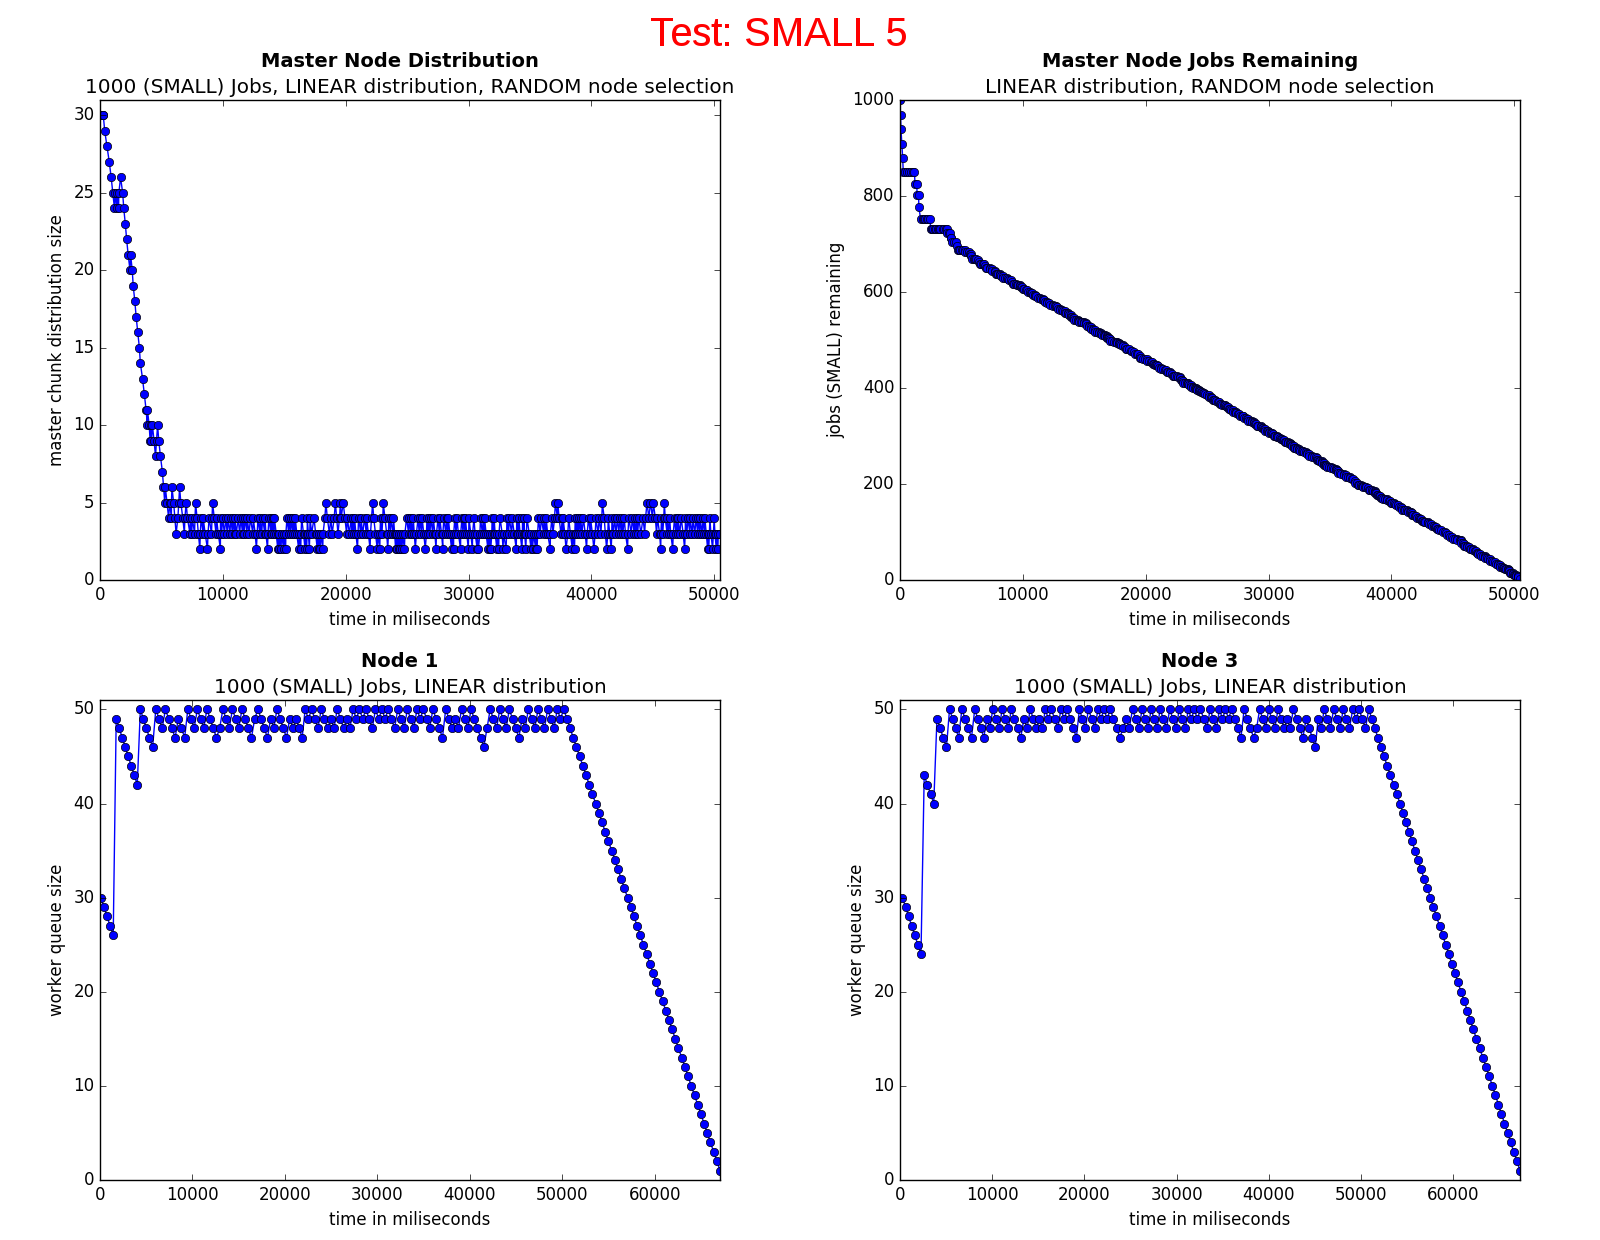
\includegraphics[width=1.2\linewidth]{combined_small_overview/case_small_5} 
    \caption{Random node selection, Linear distribution} 
    \label{testSmall5} 
    \vspace{4ex}
  \end{subfigure} 
  
  \begin{subfigure}[b]{0.5\linewidth}
    \centering
    \hbox{\hspace{-5.0em} 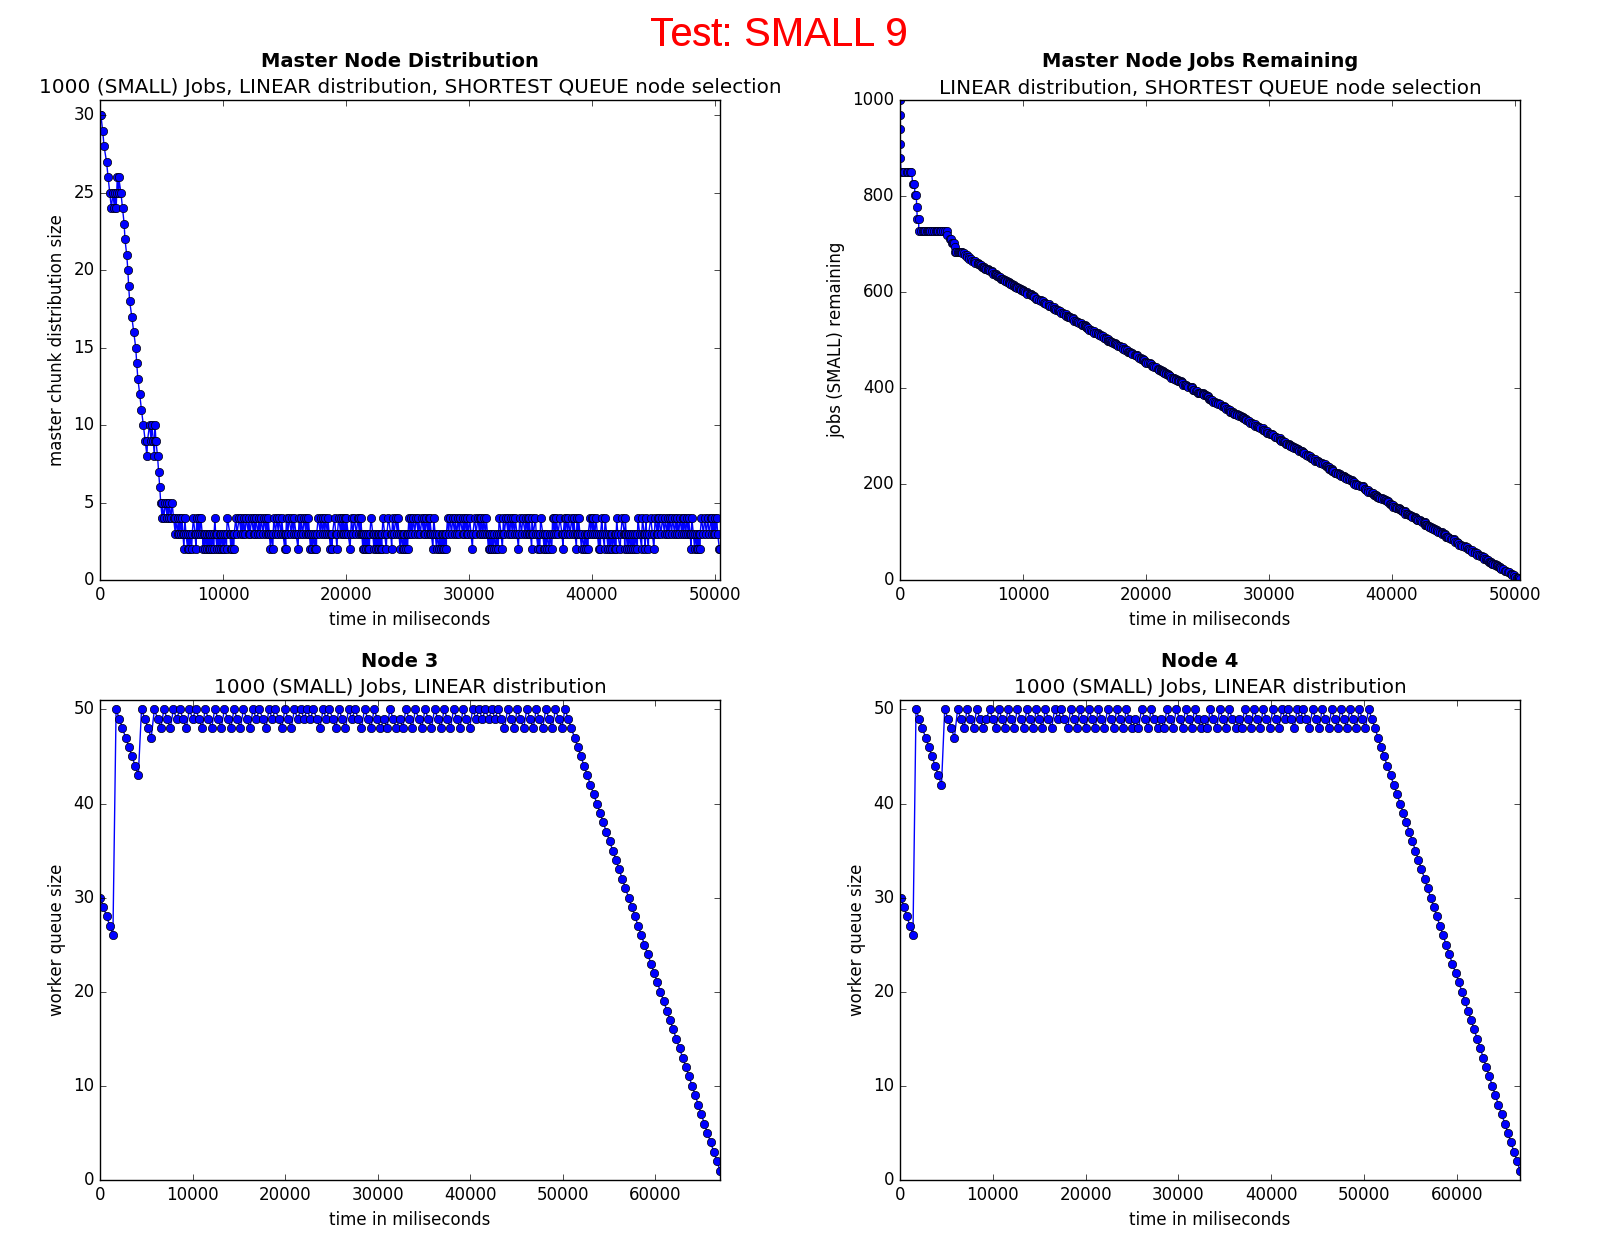
\includegraphics[width=1.2\linewidth]{combined_small_overview/case_small_9} }
    \caption{Shortest Queue node selection, Linear distribution} 
    \label{testSmall9} 
    \vspace{4ex}
  \end{subfigure}%% 
  \begin{subfigure}[b]{0.5\linewidth}
    \centering
    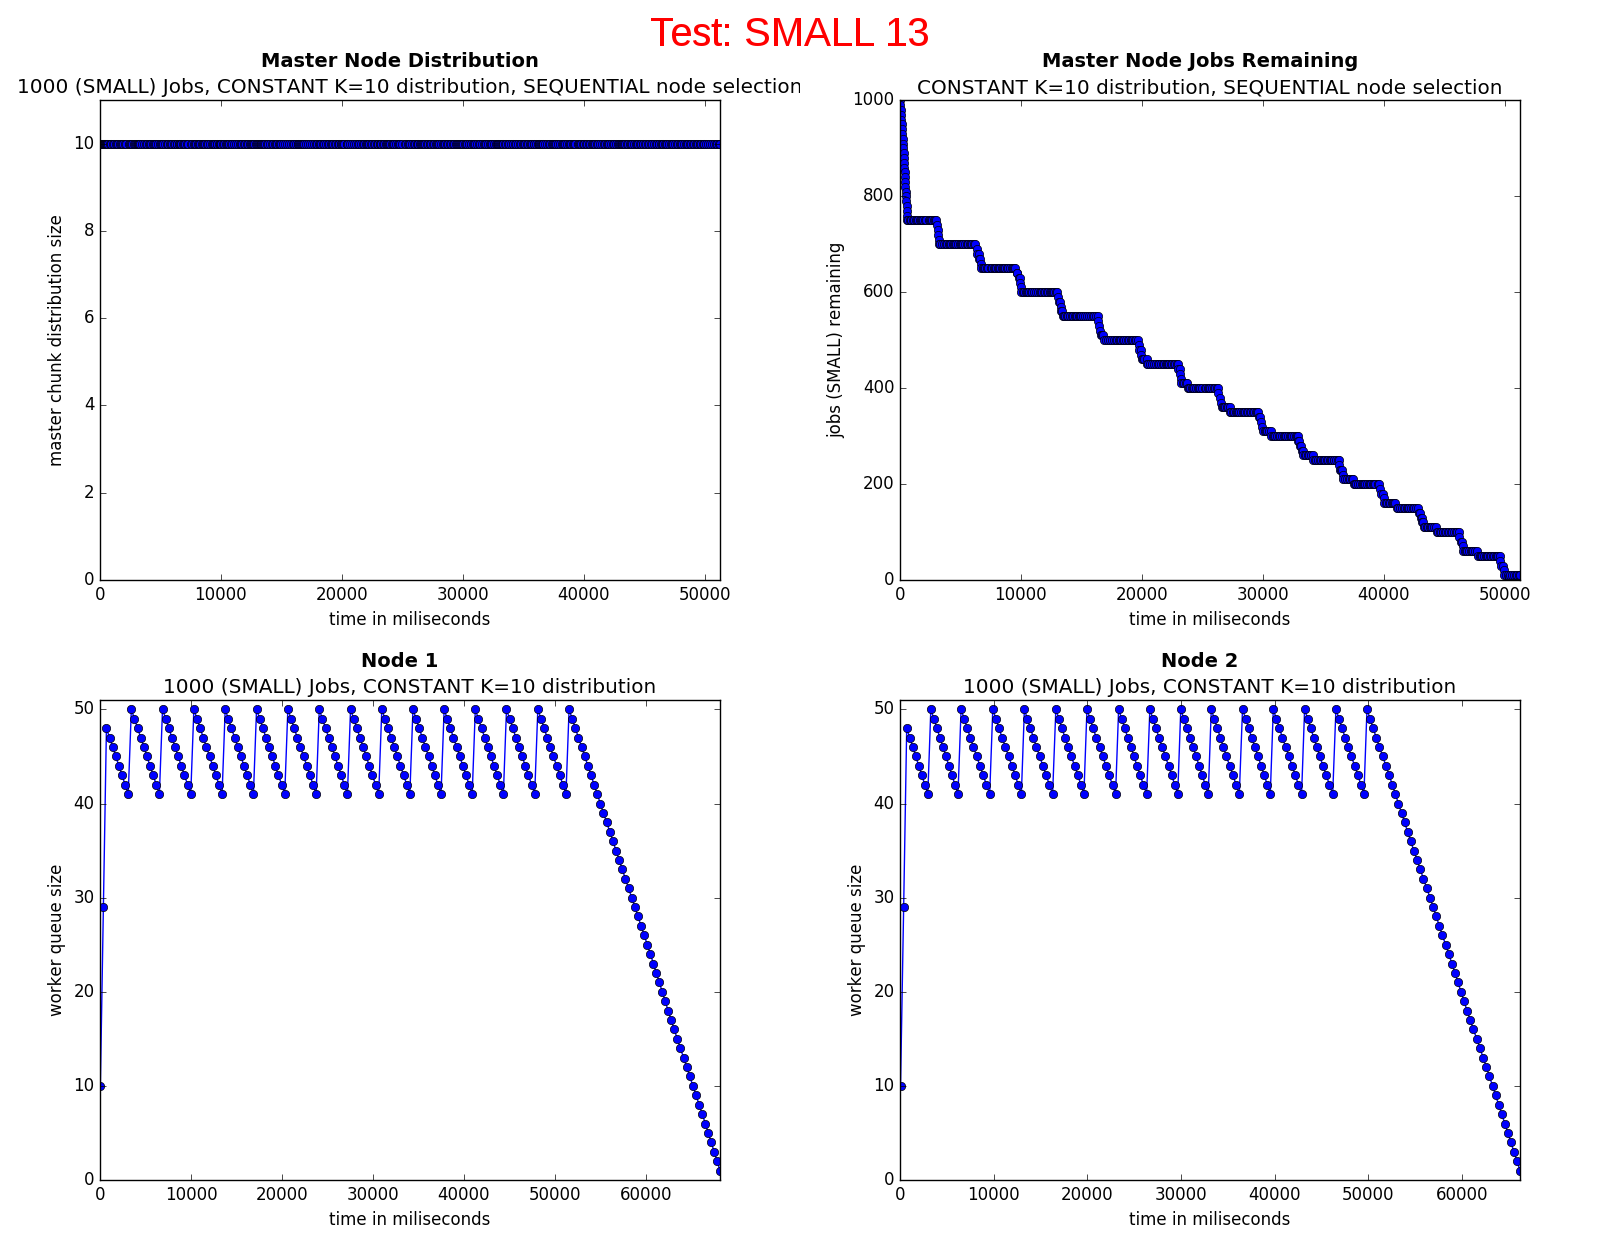
\includegraphics[width=1.2\linewidth]{combined_small_overview/case_small_13} 
    \caption{Sequential node selection, Constant distribution} 
    \label{testSmall13} 
    \vspace{4ex}
  \end{subfigure} 
  
  
  \caption{Overview of simulation with 1000 small jobs and 5 worker nodes part 1. These figures plot results for the test numbers 1, 5, 9, 13 as labeled at the top of each figure. The top left plot in each figure shows the master job distribution rate as time progresses. The top right plot in each figure shows the number of jobs remaining to distribute as time progresses. The bottom plots in each figure show queue sizes of two randomly selected workers.}
  \label{testSmall1-13} 
  
\end{figure}


\begin{figure}[p] 
  \begin{subfigure}[b]{0.5\linewidth}
    \centering
    \hbox{\hspace{-5.0em} 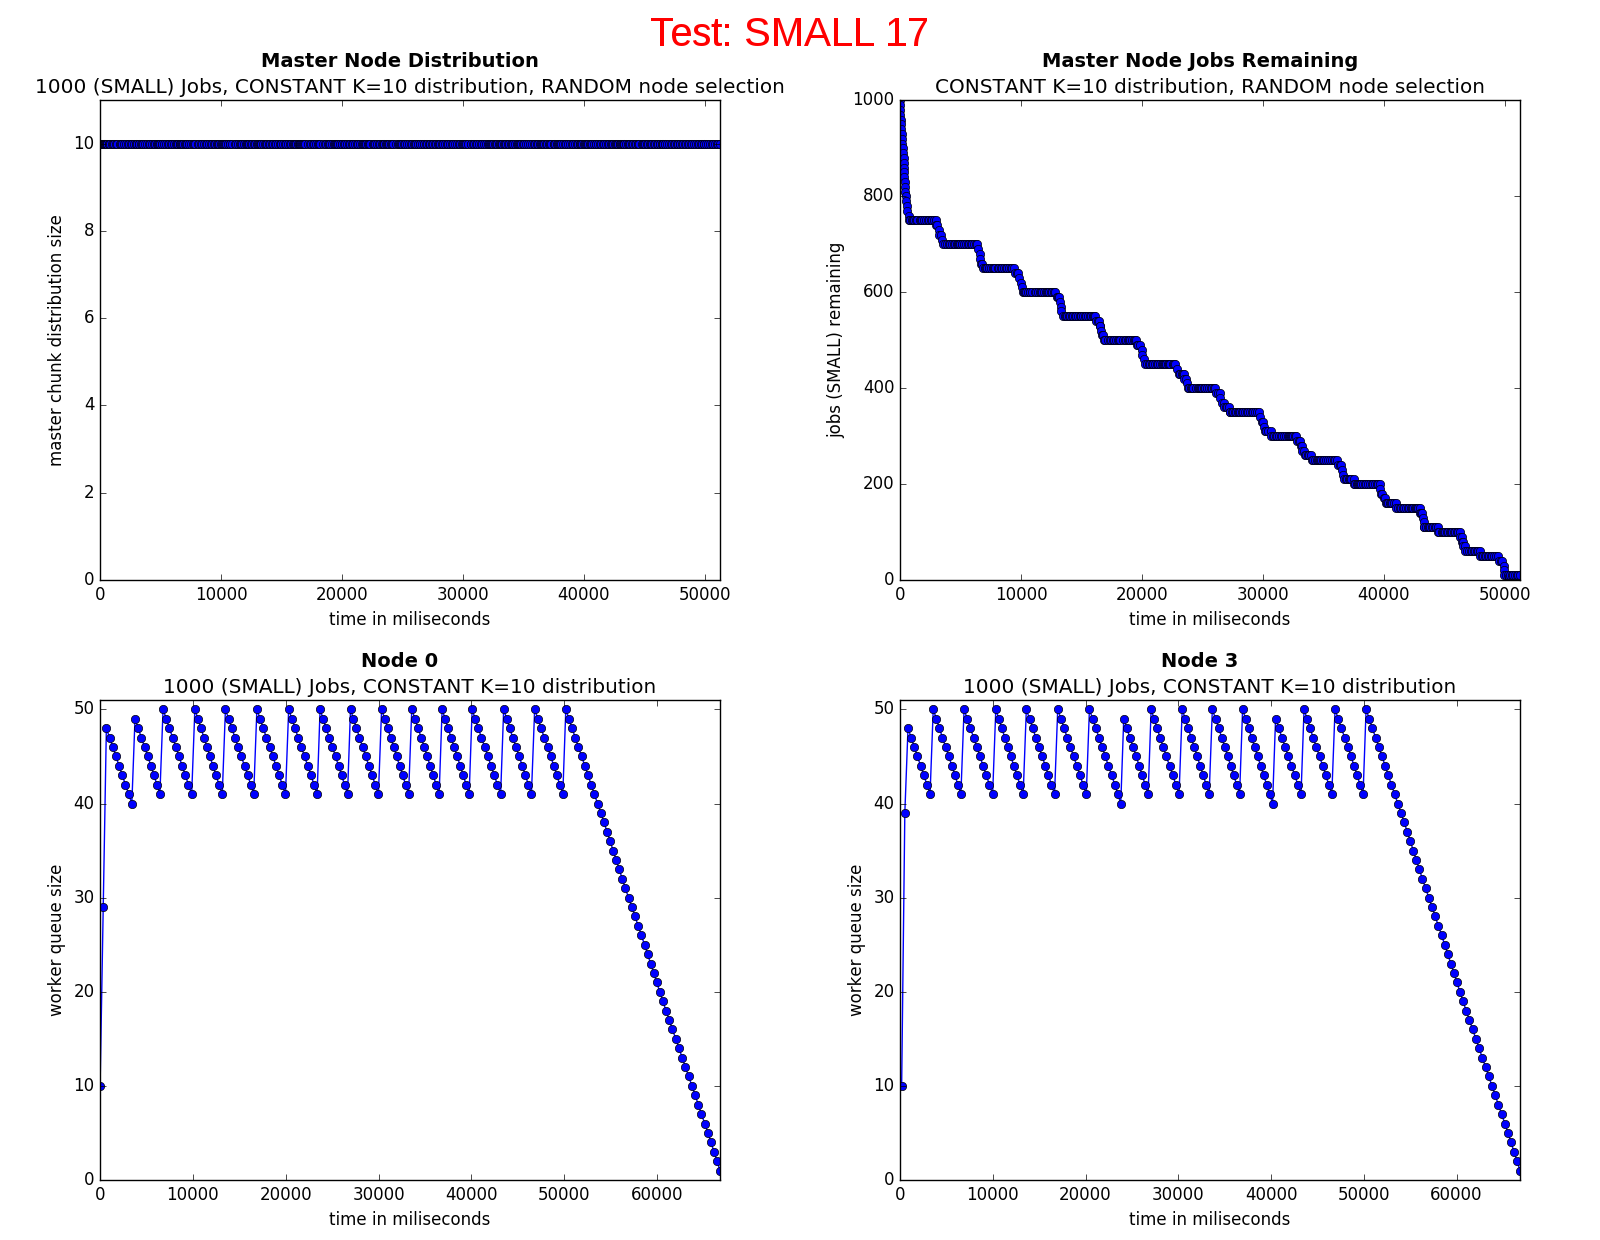
\includegraphics[width=1.2\linewidth]{combined_small_overview/case_small_17} }
    \caption{Random node selection, Constant distribution}
    \label{testSmall17} 
    \vspace{4ex}
  \end{subfigure}%% 
  \begin{subfigure}[b]{0.5\linewidth}
    \centering
    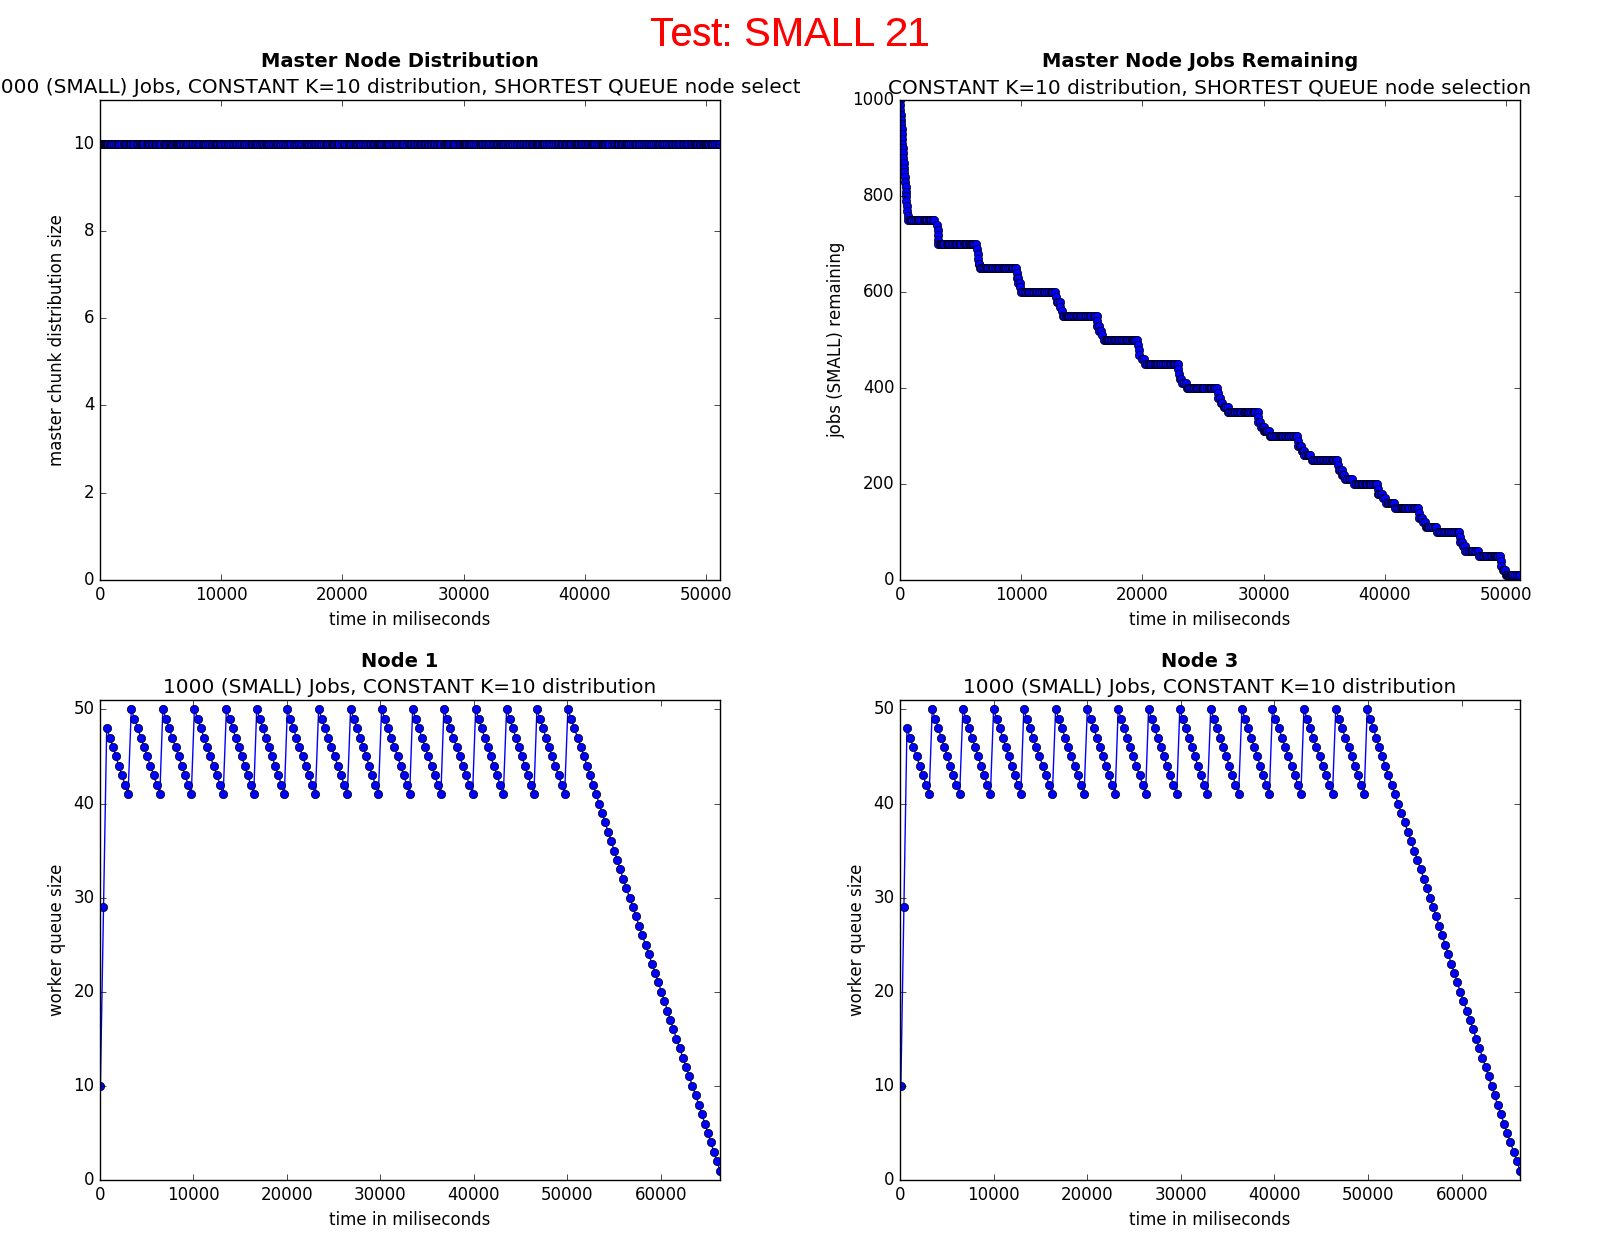
\includegraphics[width=1.2\linewidth]{combined_small_overview/case_small_21} 
    \caption{Shortest queue node selection, Constant distribution} 
    \label{testSmall21} 
    \vspace{4ex}
  \end{subfigure} 
  
  
  \begin{subfigure}[b]{0.5\linewidth}
    \centering
    \hbox{\hspace{-5.0em} 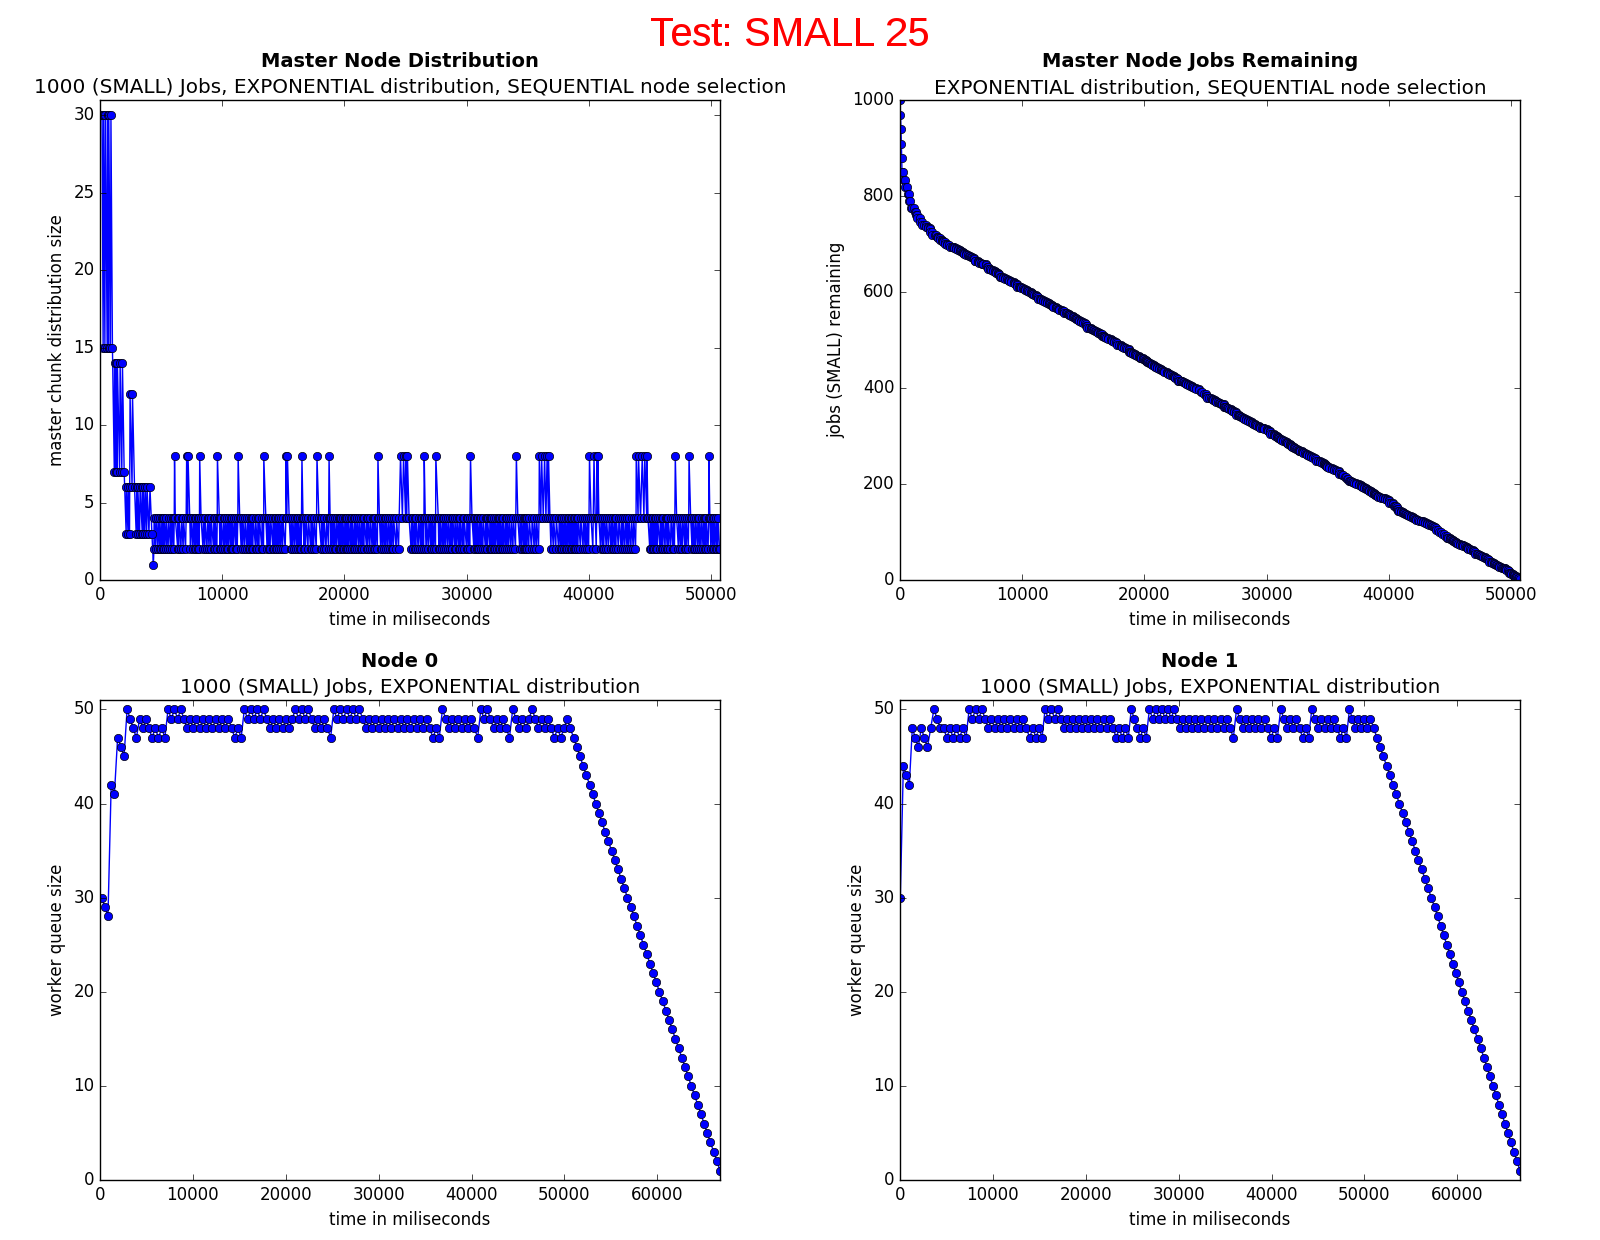
\includegraphics[width=1.2\linewidth]{combined_small_overview/case_small_25} }
    \caption{Sequential node selection, Exponential distribution} 
    \label{testSmall25} 
    \vspace{4ex}
  \end{subfigure}%% 
  \begin{subfigure}[b]{0.5\linewidth}
    \centering
    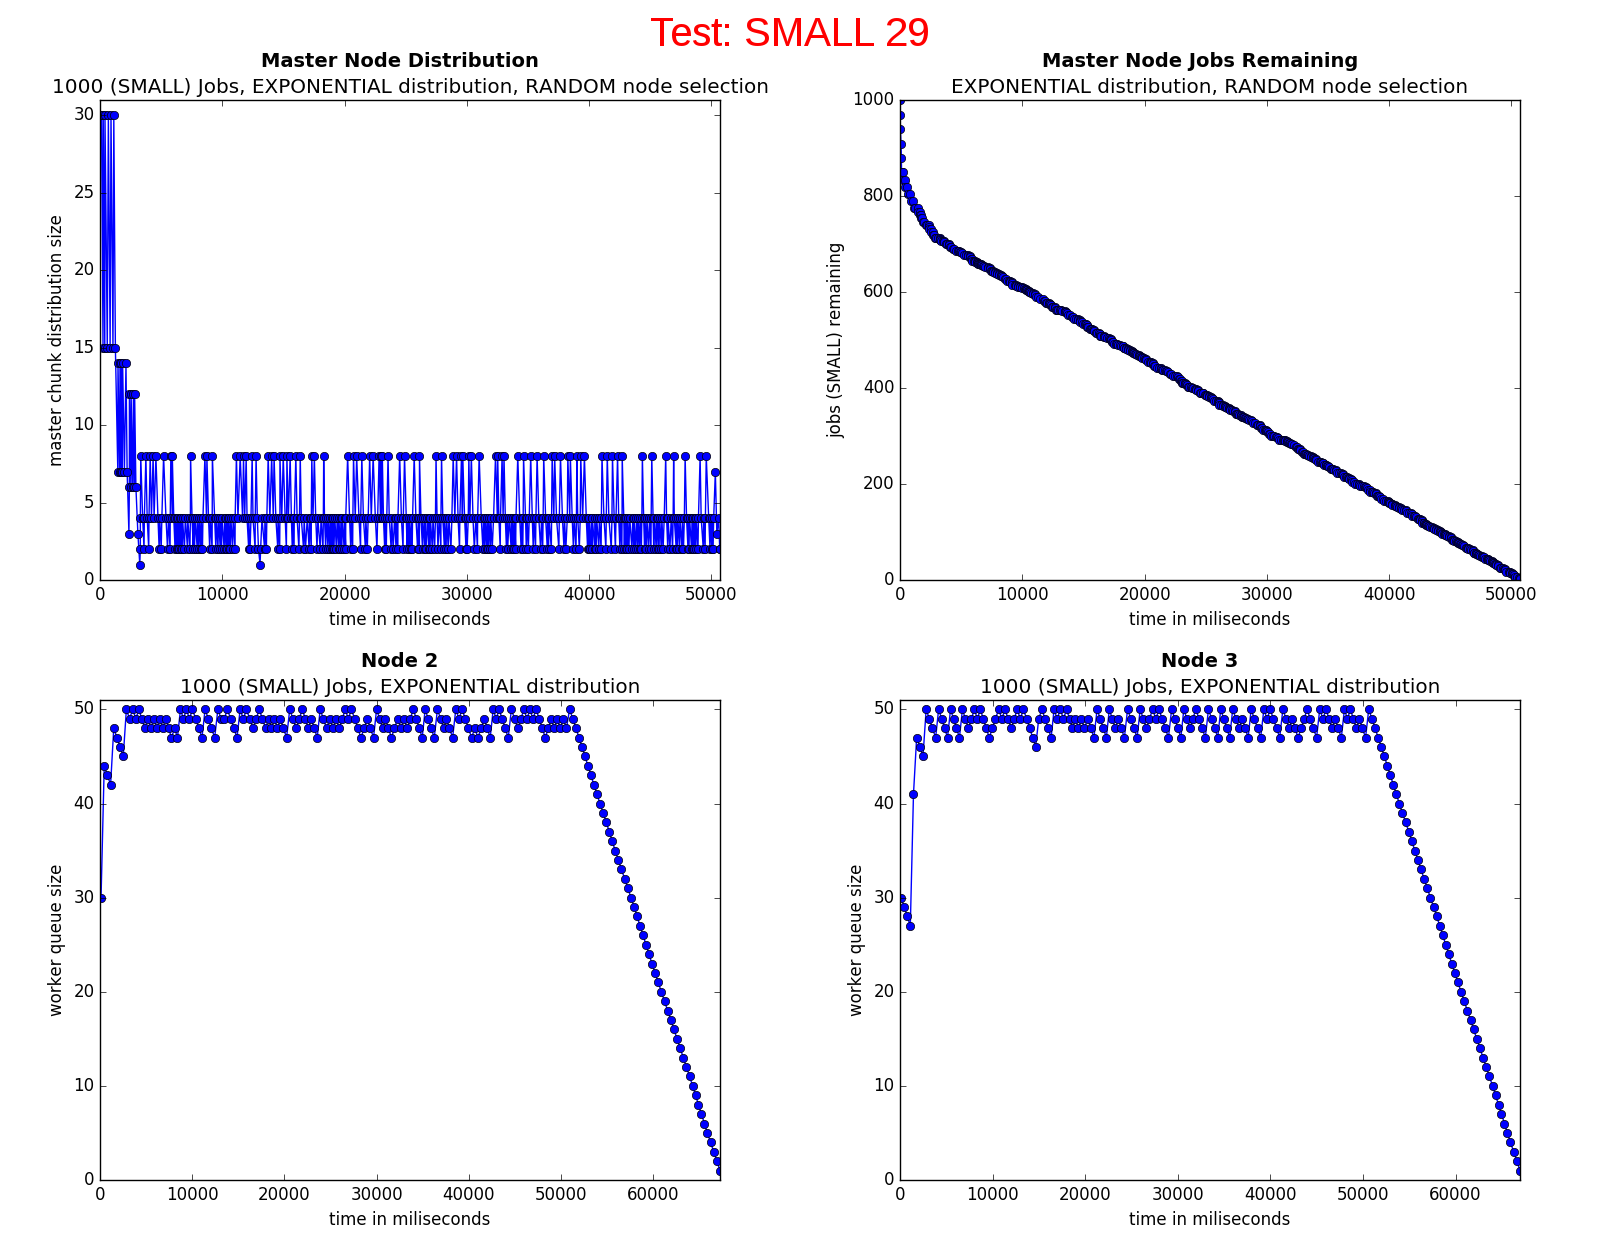
\includegraphics[width=1.2\linewidth]{combined_small_overview/case_small_29} 
    \caption{Random node selection, Exponential distribution} 
    \label{testSmall29} 
    \vspace{4ex}
  \end{subfigure} 
  
  
  \caption{Overview of simulation with 1000 small jobs and 5 worker nodes part 2. These figures plot results for the test numbers 17, 21, 25, 29 as labeled at the top of each figure. The top left plot in each figure shows the master job distribution rate as time progresses. The top right plot in each figure shows the number of jobs remaining to distribute as time progresses. The bottom plots in each figure show queue sizes of two randomly selected workers.}
  \label{testsSmall17-29} 
  
\end{figure}

\begin{figure} 
\hspace*{9em}
\begin{subfigure}[b]{0.5\linewidth}
    \centering
    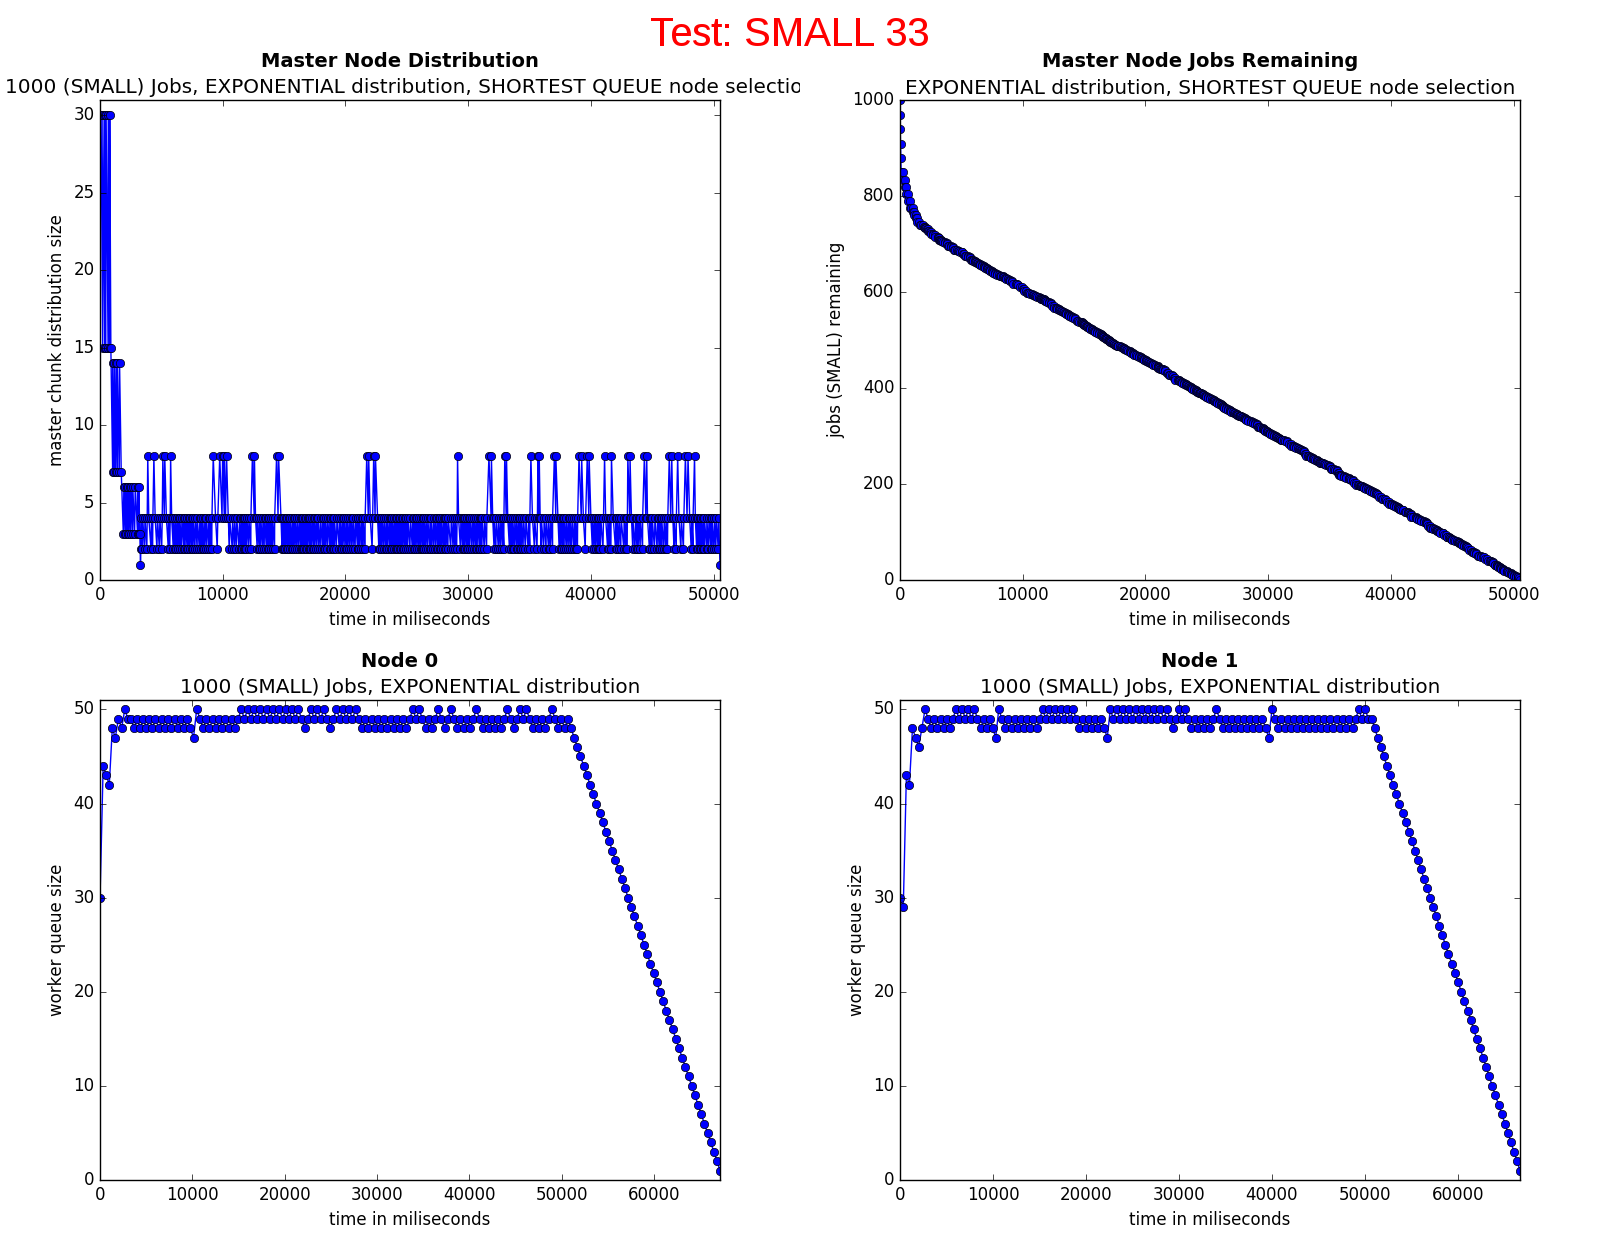
\includegraphics[scale=0.20]{combined_small_overview/case_small_33} 
    \caption{Shortest queue node selection, Exponential distribution} 
    \label{testSmall33} 
  \end{subfigure}

  \caption{Overview of simulation with 1000 small jobs and 5 worker nodes part 3. This figure plot results for the small test numbers 33 as labeled at the top of each figure. The top left plot in each figure shows the master job distribution rate as time progresses. The top right plot in each figure shows the number of jobs remaining to distribute as time progresses. The bottom plots in each figure show queue sizes of two randomly selected workers.}
  \label{testSmall33Figure} 
\end{figure}


\newpage


%%%%%%%%%%%%
% Results
%%%%%%%%%%%%

% OK
\section{Results: 1000 Small Jobs} \label{1000SmallJobs}

Table \ref{smallJobsTable} shows all the test configurations for 1000 small jobs. The last two columns specify the execution time as well as the estimated sequential execution time. Figures \ref{testSmall1-13}, \ref{testsSmall17-29}, \ref{testSmall33Figure} show an overview of results where 5 worker nodes were used.

When there are more workers for each of the job distribution strategies, as shown in Figures \ref{testsSmallExp}, \ref{testsSmallLinear}, \ref{testsSmallConstant}, master clearly takes less time to execute, since it is quicker to distribute jobs when there are more workers present to receive jobs.

% OK
\subsection{Varying Node Selection} \label{smallNodeSelection}
In order to determine the effects of node selection, the tests where job distribution remained unchanged were looked at. In particular, Figures \ref{testSmall1}, \ref{testSmall5}, \ref{testSmall9} are tests where job distribution remains linear. The two bottom plots of each figure, which are the node plots, do not seem to have much variation. The same goes for Figures \ref{testSmall13}, \ref{testSmall17}, \ref{testSmall21}, where job distribution is constant and Figures \ref{testSmall25}, \ref{testSmall29}, \ref{testSmall33} where job distribution is exponential. In order to further dive deep into the results, the plots with higher worker counts (not shown in the report) were analyzed and also did not show any variation. The reason for the lack of impact on the plots could be due to the fact that this is a simulation of the ideal environment.

The other piece of data to inspect besides the plots is the timing of these configurations. Test cases 1 through 12 in Table \ref{smallJobsTable} represent linear job distribution but varying node selection. Looking at the tests where node selection differs yet the number of workers is the same, such as tests 2, 5, 10, it is evident that random node selection performs around 0.5 second worse than sequential and shortest queue distributions. Sequential and shortest queue strategies tend to perform similarly. The same can be noticed when looking at tests 3, 6, 11 and 4, 7, 12 and when repeating this inspection on tests 13-24 and 25-36. The reason sequential and shortest queue node selections perform better is due to the fact that random node selection has a higher chance of selecting the same node as previously selected, which becomes detrimental when worker queues are at maximum capacity.

% OK
\subsection{Varying Job Distribution Strategy} \label{smallJobDistribution}
Figure \ref{testsSmallLinear} shows how the linear job chunk distribution strategy performs as the number of workers grow on 1000 small jobs. As pointed out in Table \ref{smallJobsTable}, the tests 1, 2, 3, 4 which are shown in Figure \ref{testsSmallLinear} start at taking around 67 seconds and shrink down to around 22 seconds. 

Figure \ref{testsSmallExp} shows how the exponential job chunk distribution strategy performs as the number of workers grow on 1000 small jobs. As pointed out in Table \ref{smallJobsTable}, the tests 25, 26, 27, 28 which are shown in Figure \ref{testsSmallExp} start at taking around 67 seconds and shrink down to around 23 seconds.

Figure \ref{testsSmallConstant} shows how the constant job chunk distribution strategy performs as the number of workers grow on 1000 small jobs. As pointed out in Table \ref{smallJobsTable}, the tests 13, 14, 15, 16 which are shown in Figure \ref{testsSmallConstant} start at taking around 68 seconds and shrink down to around 18 seconds. 

Looking at Table \ref{smallJobsTable} overall, it seems that as far as execution time goes, constant strategy performs the best out of all distribution strategies. This may be due to the case that with the constant method when there are a larger number of workers available the worker queue sizes will be increased by the constant job chunk size of 10, while in linear and exponential cases the job chunk size is very likely to be at the maximum setting of 30 thus making some workers execute longer.

% OK
\subsubsection{Linear Job Distribution} \label{smallJobDistributionLinear}

As the number of workers grow from Figure \ref{testLinearSmall5} to Figure \ref{testLinearSmall30}, the variation in job chunk size, as shown by the top left plot in each figure, is clearly becoming smaller. In Figure \ref{testLinearSmall5} the job chunk is initially around 30 jobs, but quickly drops down to 1 or 2 jobs. While in Figure \ref{testLinearSmall30} there is much less variation as the number of jobs being distributed stays roughly around 25 jobs. This makes sense as there are more workers to distribute jobs to, thus in the time that it takes master to distribute chunks to some workers, other workers had time to process some of their jobs.

What is also interesting to point out is that as the number of workers grow, the plots showing the number of jobs remaining become less and less smooth. In Figure \ref{testLinearSmall5} the top right plot shows a somewhat smooth descent while in Figure \ref{testLinearSmall30} the top right plot shows a smooth descent initially and then is disrupted for a little while. This implies that during those times job chunk size must have been dropping, and that is the case as shown by Figure \ref{testLinearSmall30} where around the time where the top right plot has a horizontal line, the top left plot is showing a drop in job chunk size.

% OK
\subsubsection{Exponential Job Distribution} \label{smallJobDistributionExp} 

The two points regarding variation in job chunk size and smoothness of the plot showing number of jobs remaining also apply to the exponential distribution. What varies though is that for tests with higher number of workers, such as Figures \ref{testExpSmall20}, \ref{testExpSmall30}, the variation is a bit bigger than in the linear case due to the fact that exponential strategy works by doubling and halving the job chunk size.

% OK
\subsubsection{Constant Job Distribution} \label{smallJobDistributionConstant}

Unlike in the case of linear or exponential, the job descent occurs in a much more stepwise manner as shown in Figures \ref{testConstantSmall5}, \ref{testConstantSmall10}. In Figures \ref{testConstantSmall20}, \ref{testConstantSmall30} the bottom plots of each figure demonstrate that the worker queue sizes will only grow by the constant rate thus avoiding sudden large workload sizes as demonstrated by linear and exponential distributions.

% OK
\section{Results: 1000 Mid/Large Jobs} \label{1000MidLargeJobs}
The same exact testing as shown in Table \ref{smallJobsTable} was done with mid and large sized jobs. After looking through the data, the results were not much different from what was already discussed in the analysis of 1000 small jobs. Hence the data and plots have not been included in this report, but are available in the project repository for inspection.


%============================== START SMALL Data Table
%=================================================
\begin{table}

\hspace*{-4em}
\begin{tabular}{|c | c | c | c | c | c | c |}
\hline
\textbf{Test \#} & \textbf{Job Number} & \textbf{\# of Workers} & \textbf{Node} & \textbf{Distribution} & \textbf{Execution} & \textbf{Sequential} \\

 & \textbf{\& Size} &  & \textbf{Selection} &  & \textbf{Time (sec)} & \textbf{Time (sec)} \\

\hline
1  & 1000 SMALL JOBS & 5  & SEQUENTIAL & LINEAR            & 67.52325  & 320.64  \\ \hline
2  & 1000 SMALL JOBS & 10 & SEQUENTIAL & LINEAR            & 37.449792 & 320.663 \\ \hline
3  & 1000 SMALL JOBS & 20 & SEQUENTIAL & LINEAR            & 22.213429 & 320.626 \\ \hline
4  & 1000 SMALL JOBS & 30 & SEQUENTIAL & LINEAR            & 22.88186  & 320.749 \\ \hline
   &                 &    &            &                   &           &         \\ \hline
5  & 1000 SMALL JOBS & 5  & RANDOM     & LINEAR            & 67.548033 & 320.557 \\ \hline
6  & 1000 SMALL JOBS & 10 & RANDOM     & LINEAR            & 38.254254 & 321.306 \\ \hline
7  & 1000 SMALL JOBS & 20 & RANDOM     & LINEAR            & 22.682357 & 320.759 \\ \hline
8  & 1000 SMALL JOBS & 30 & RANDOM     & LINEAR            & 23.76065  & 321.227 \\ \hline
   &                 &    &            &                   &           &         \\ \hline
9  & 1000 SMALL JOBS & 5  & SQS        & LINEAR            & 67.556903 & 320.532 \\ \hline
10 & 1000 SMALL JOBS & 10 & SQS        & LINEAR            & 37.937056 & 320.745 \\ \hline
11 & 1000 SMALL JOBS & 20 & SQS        & LINEAR            & 22.250906 & 320.485 \\ \hline
12 & 1000 SMALL JOBS & 30 & SQS        & LINEAR            & 23.883818 & 321.599 \\ \hline
   &                 &    &            &                   &           &         \\ \hline
13 & 1000 SMALL JOBS & 5  & SEQUENTIAL & CONSTANT (K = 10) & 68.455644 & 320.276 \\ \hline
14 & 1000 SMALL JOBS & 10 & SEQUENTIAL & CONSTANT (K = 10) & 36.764797 & 320.393 \\ \hline
15 & 1000 SMALL JOBS & 20 & SEQUENTIAL & CONSTANT (K = 10) & 18.851795 & 321.838 \\ \hline
16 & 1000 SMALL JOBS & 30 & SEQUENTIAL & CONSTANT (K = 10) & 18.298678 & 320.765 \\ \hline
   &                 &    &            &                   &           &         \\ \hline
17 & 1000 SMALL JOBS & 5  & RANDOM     & CONSTANT (K = 10) & 68.715863 & 320.684 \\ \hline
18 & 1000 SMALL JOBS & 10 & RANDOM     & CONSTANT (K = 10) & 37.237259 & 321.706 \\ \hline
19 & 1000 SMALL JOBS & 20 & RANDOM     & CONSTANT (K = 10) & 21.887619 & 320.886 \\ \hline
20 & 1000 SMALL JOBS & 30 & RANDOM     & CONSTANT (K = 10) & 20.737932 & 320.615 \\ \hline
   &                 &    &            &                   &           &         \\ \hline
21 & 1000 SMALL JOBS & 5  & SQS        & CONSTANT (K = 10) & 68.596678 & 320.484 \\ \hline
22 & 1000 SMALL JOBS & 10 & SQS        & CONSTANT (K = 10) & 36.807229 & 320.732 \\ \hline
23 & 1000 SMALL JOBS & 20 & SQS        & CONSTANT (K = 10) & 18.706516 & 321.487 \\ \hline
24 & 1000 SMALL JOBS & 30 & SQS        & CONSTANT (K = 10) & 17.415236 & 320.802 \\ \hline
   &                 &    &            &                   &           &         \\ \hline
25 & 1000 SMALL JOBS & 5  & SEQUENTIAL & EXP               & 67.439778 & 321.095 \\ \hline
26 & 1000 SMALL JOBS & 10 & SEQUENTIAL & EXP               & 37.614362 & 320.896 \\ \hline
27 & 1000 SMALL JOBS & 20 & SEQUENTIAL & EXP               & 22.393486 & 321.518 \\ \hline
28 & 1000 SMALL JOBS & 30 & SEQUENTIAL & EXP               & 23.397359 & 321.743 \\ \hline
   &                 &    &            &                   &           &         \\ \hline
29 & 1000 SMALL JOBS & 5  & RANDOM     & EXP               & 67.554958 & 320.581 \\ \hline
30 & 1000 SMALL JOBS & 10 & RANDOM     & EXP               & 38.649991 & 320.255 \\ \hline
31 & 1000 SMALL JOBS & 20 & RANDOM     & EXP               & 22.816328 & 320.638 \\ \hline
32 & 1000 SMALL JOBS & 30 & RANDOM     & EXP               & 22.246627 & 320.45  \\ \hline
   &                 &    &            &                   &           &         \\ \hline
33 & 1000 SMALL JOBS & 5  & SQS        & EXP               & 67.476154 & 320.872 \\ \hline
34 & 1000 SMALL JOBS & 10 & SQS        & EXP               & 37.554753 & 320.53  \\ \hline
35 & 1000 SMALL JOBS & 20 & SQS        & EXP               & 22.29204  & 320.773 \\ \hline
36 & 1000 SMALL JOBS & 30 & SQS        & EXP               & 23.512812 & 320.611 \\ 
\hline
\end{tabular}

\caption{Listing of all test cases ran on 1000 small jobs. \label{smallJobsTable}}
\end{table}
%============================== END SMALL Data Table
%=================================================


%============================== START SMALL Exponential FIGURES
%=================================================

\begin{figure}[p] 
  \begin{subfigure}[b]{0.5\linewidth}
    \centering
    \hbox{\hspace{-5.0em} 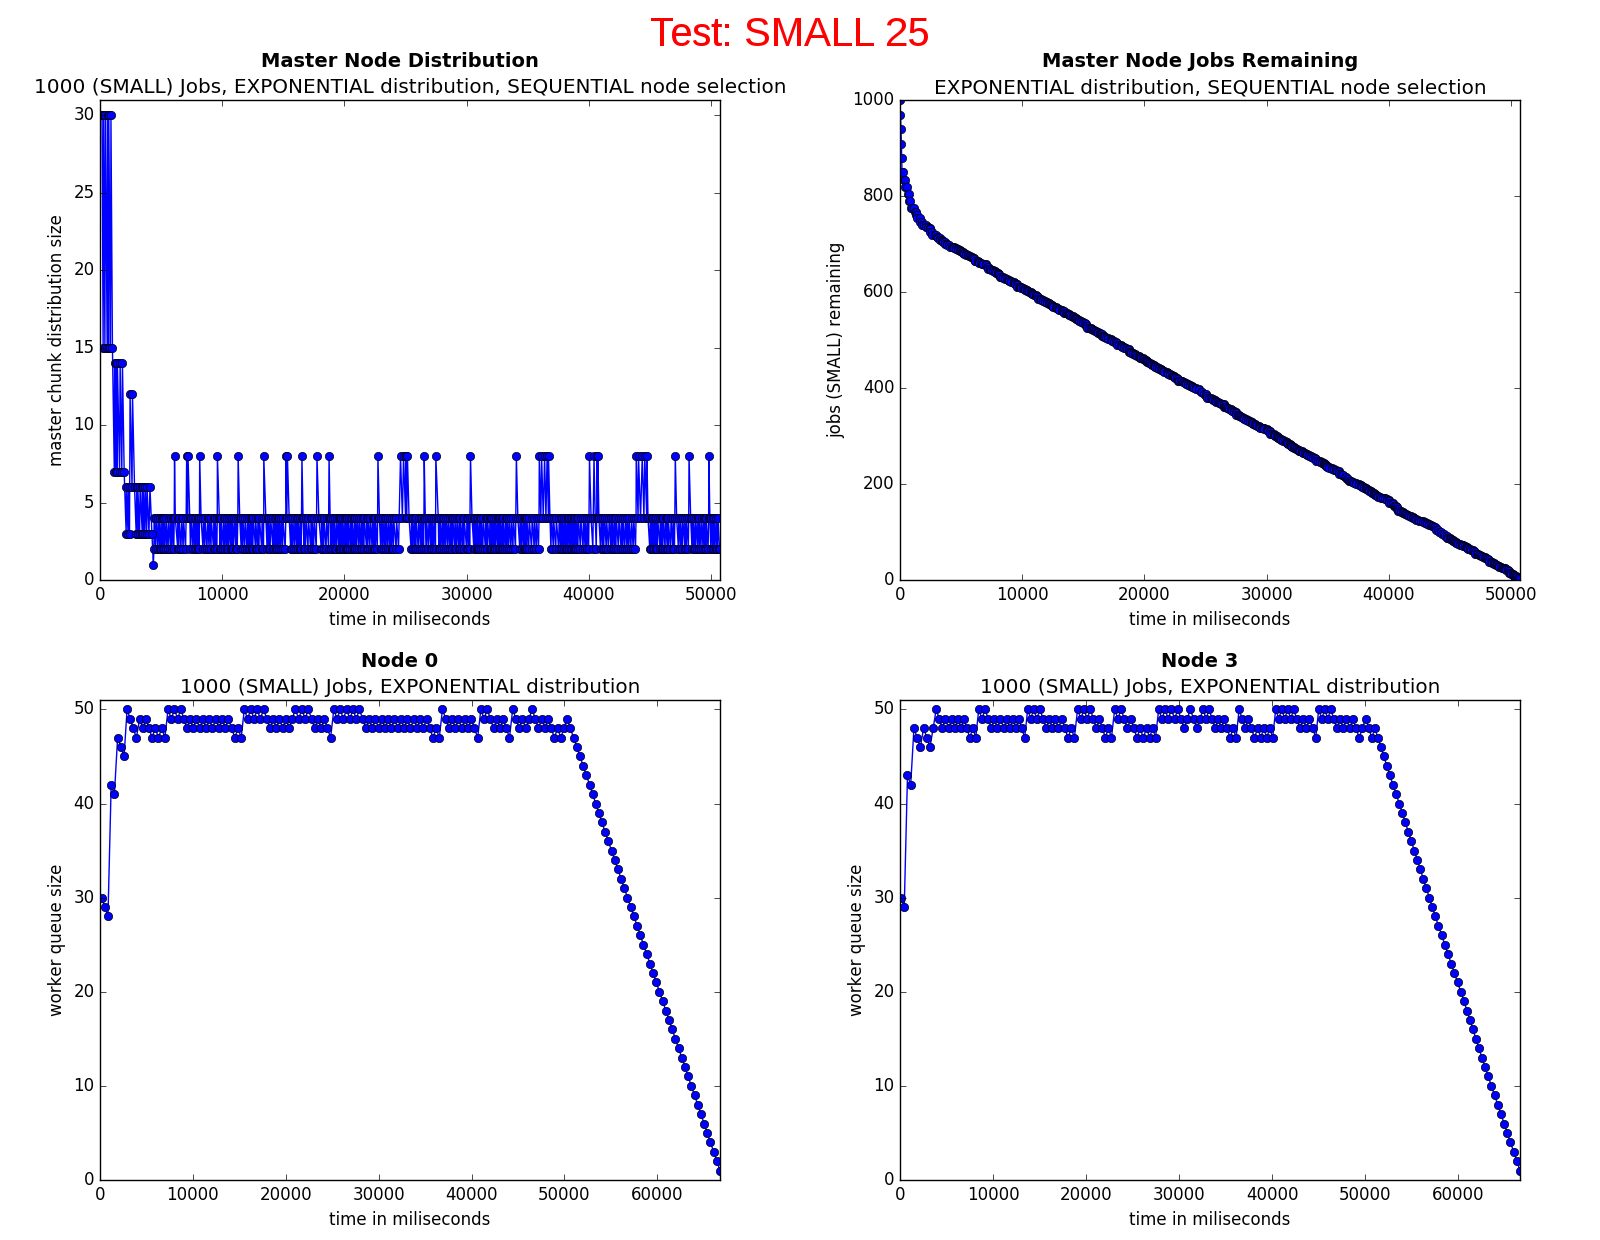
\includegraphics[width=1.2\linewidth]{combined_small_growing_workers_exp/case_small_25} }
    \caption{5 workers}
    \label{testExpSmall5} 
    \vspace{4ex}
  \end{subfigure}%% 
  \begin{subfigure}[b]{0.5\linewidth}
    \centering
    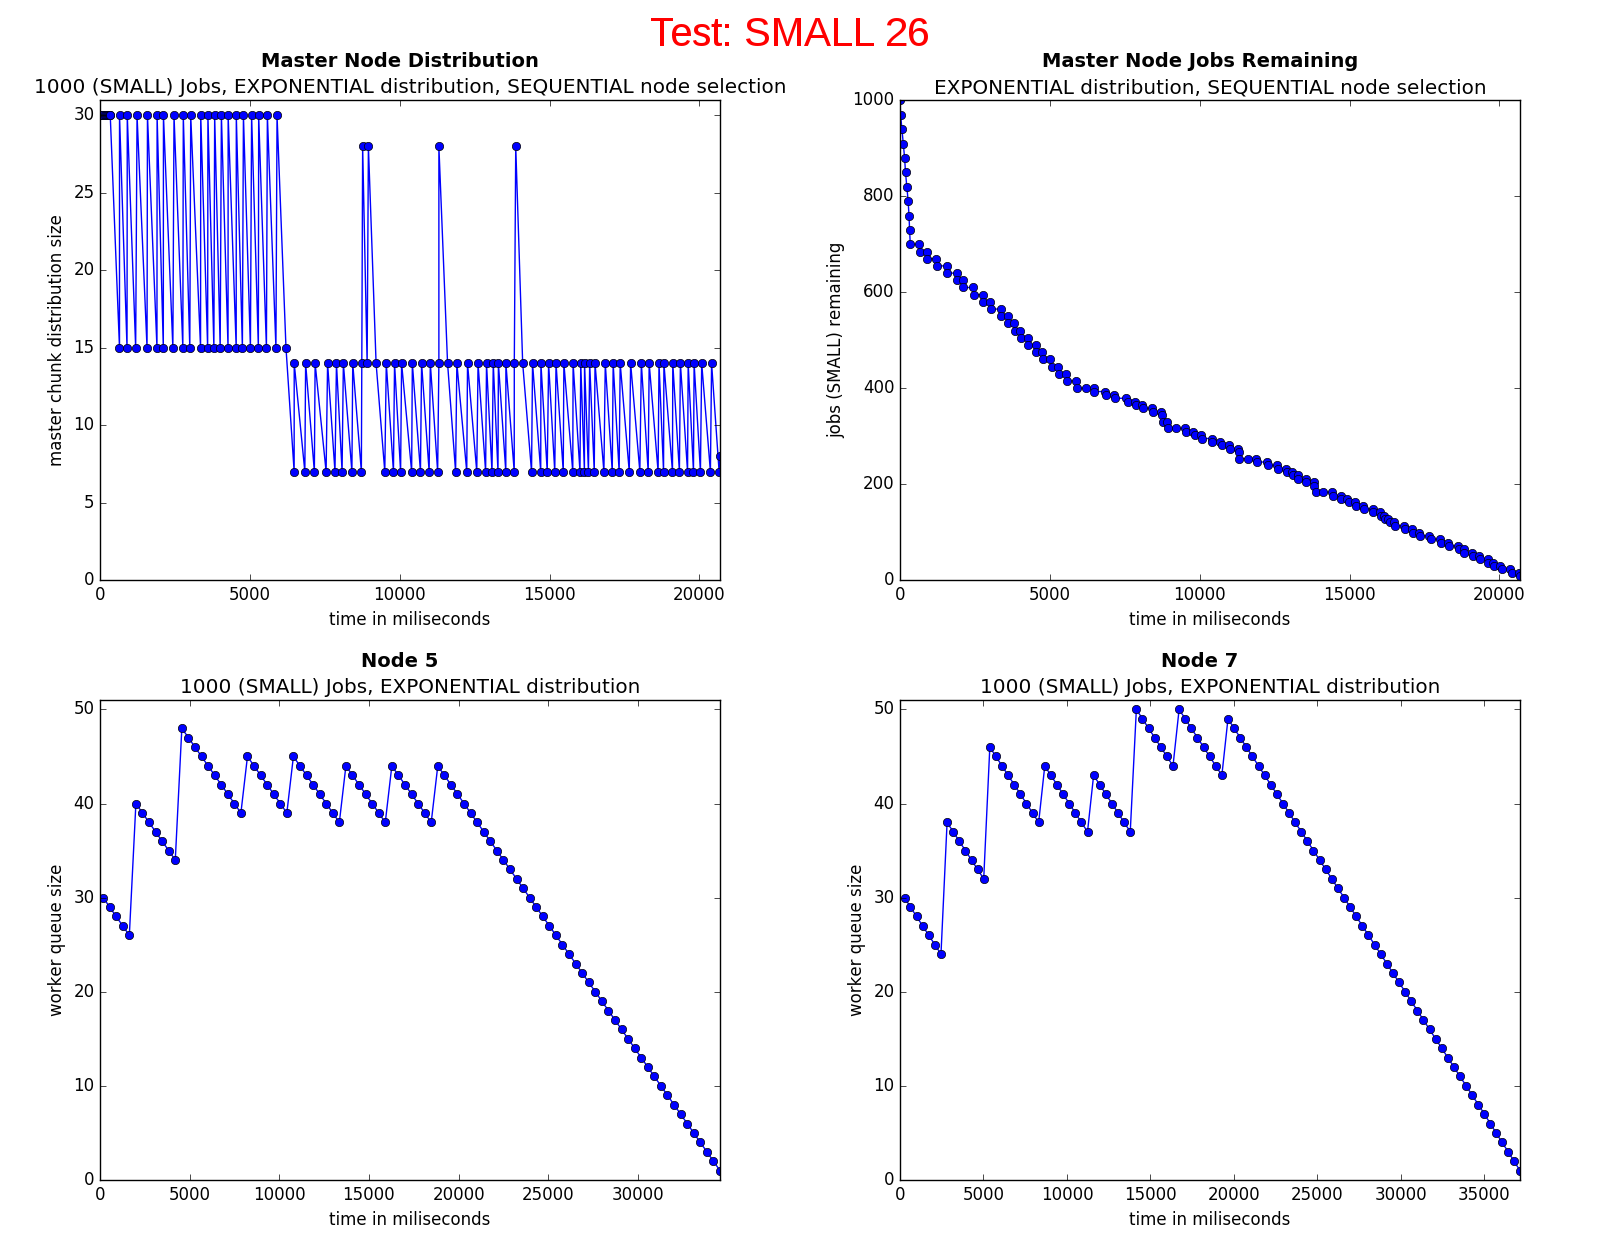
\includegraphics[width=1.2\linewidth]{combined_small_growing_workers_exp/case_small_26} 
    \caption{10 workers} 
    \label{testExpSmall10} 
    \vspace{4ex}
  \end{subfigure} 
  
  
  \begin{subfigure}[b]{0.5\linewidth}
    \centering
    \hbox{\hspace{-5.0em} 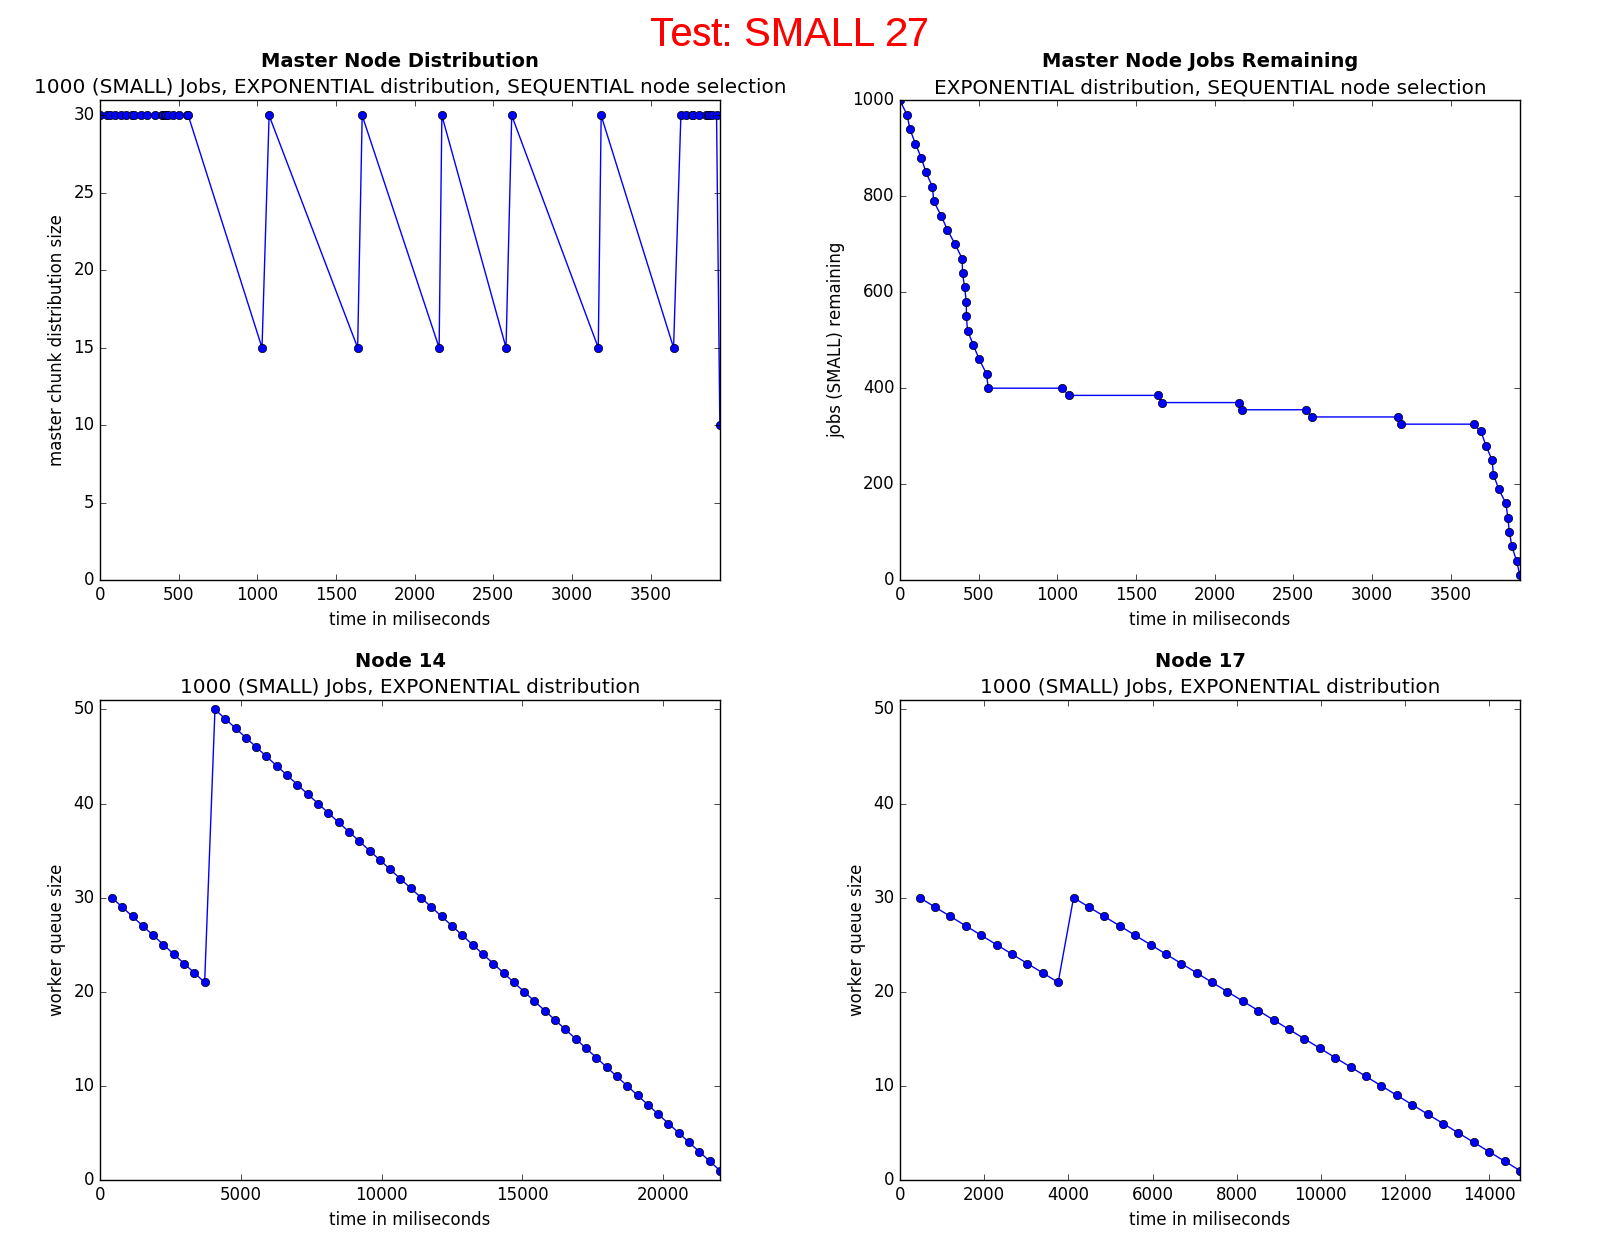
\includegraphics[width=1.2\linewidth]{combined_small_growing_workers_exp/case_small_27} }
    \caption{20 workers} 
    \label{testExpSmall20} 
    \vspace{4ex}
  \end{subfigure}%% 
  \begin{subfigure}[b]{0.5\linewidth}
    \centering
    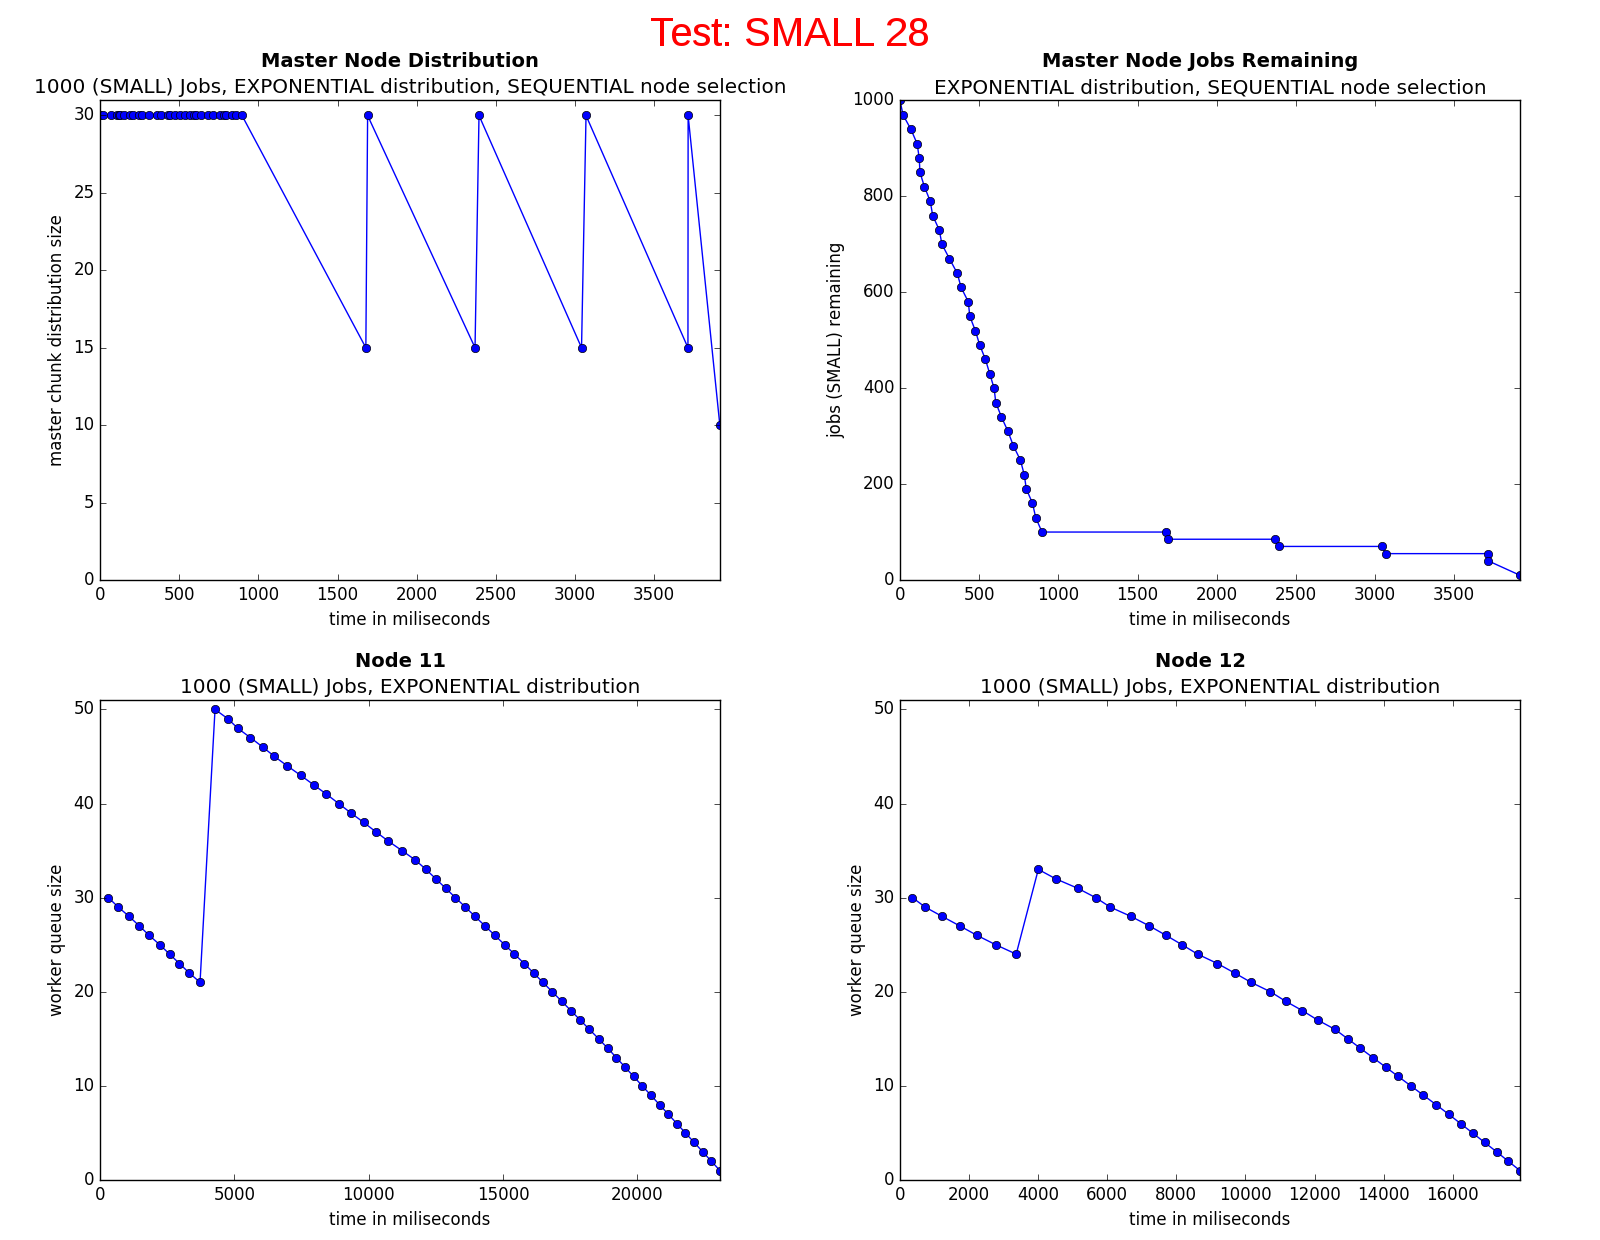
\includegraphics[width=1.2\linewidth]{combined_small_growing_workers_exp/case_small_28} 
    \caption{30 workers} 
    \label{testExpSmall30} 
    \vspace{4ex}
  \end{subfigure} 
  
  
  \caption{These tests focus on exponential job chunk distribution with 1000 small jobs to process and varying worker size. The figures plot results for the small test numbers 25, 26, 27, 28 as labeled at the top of each figure. The top left plot in each figure shows the master job distribution rate as time progresses. The top right plot in each figure shows the number of jobs remaining to distribute as time progresses. The bottom plots in each figure show queue sizes of two randomly selected workers.}
  \label{testsSmallExp} 
  
\end{figure}
%============================== END SMALL Exponential FIGURES
%=================================================


%============================== START SMALL Linear FIGURES
%=================================================
\begin{figure}[p] 
  \begin{subfigure}[b]{0.5\linewidth}
    \centering
    \hbox{\hspace{-5.0em} \includegraphics[width=1.2\linewidth]{combined_small_growing_workers_linear/case_small_1} }
    \caption{5 workers}
    \label{testLinearSmall5} 
    \vspace{4ex}
  \end{subfigure}%% 
  \begin{subfigure}[b]{0.5\linewidth}
    \centering
    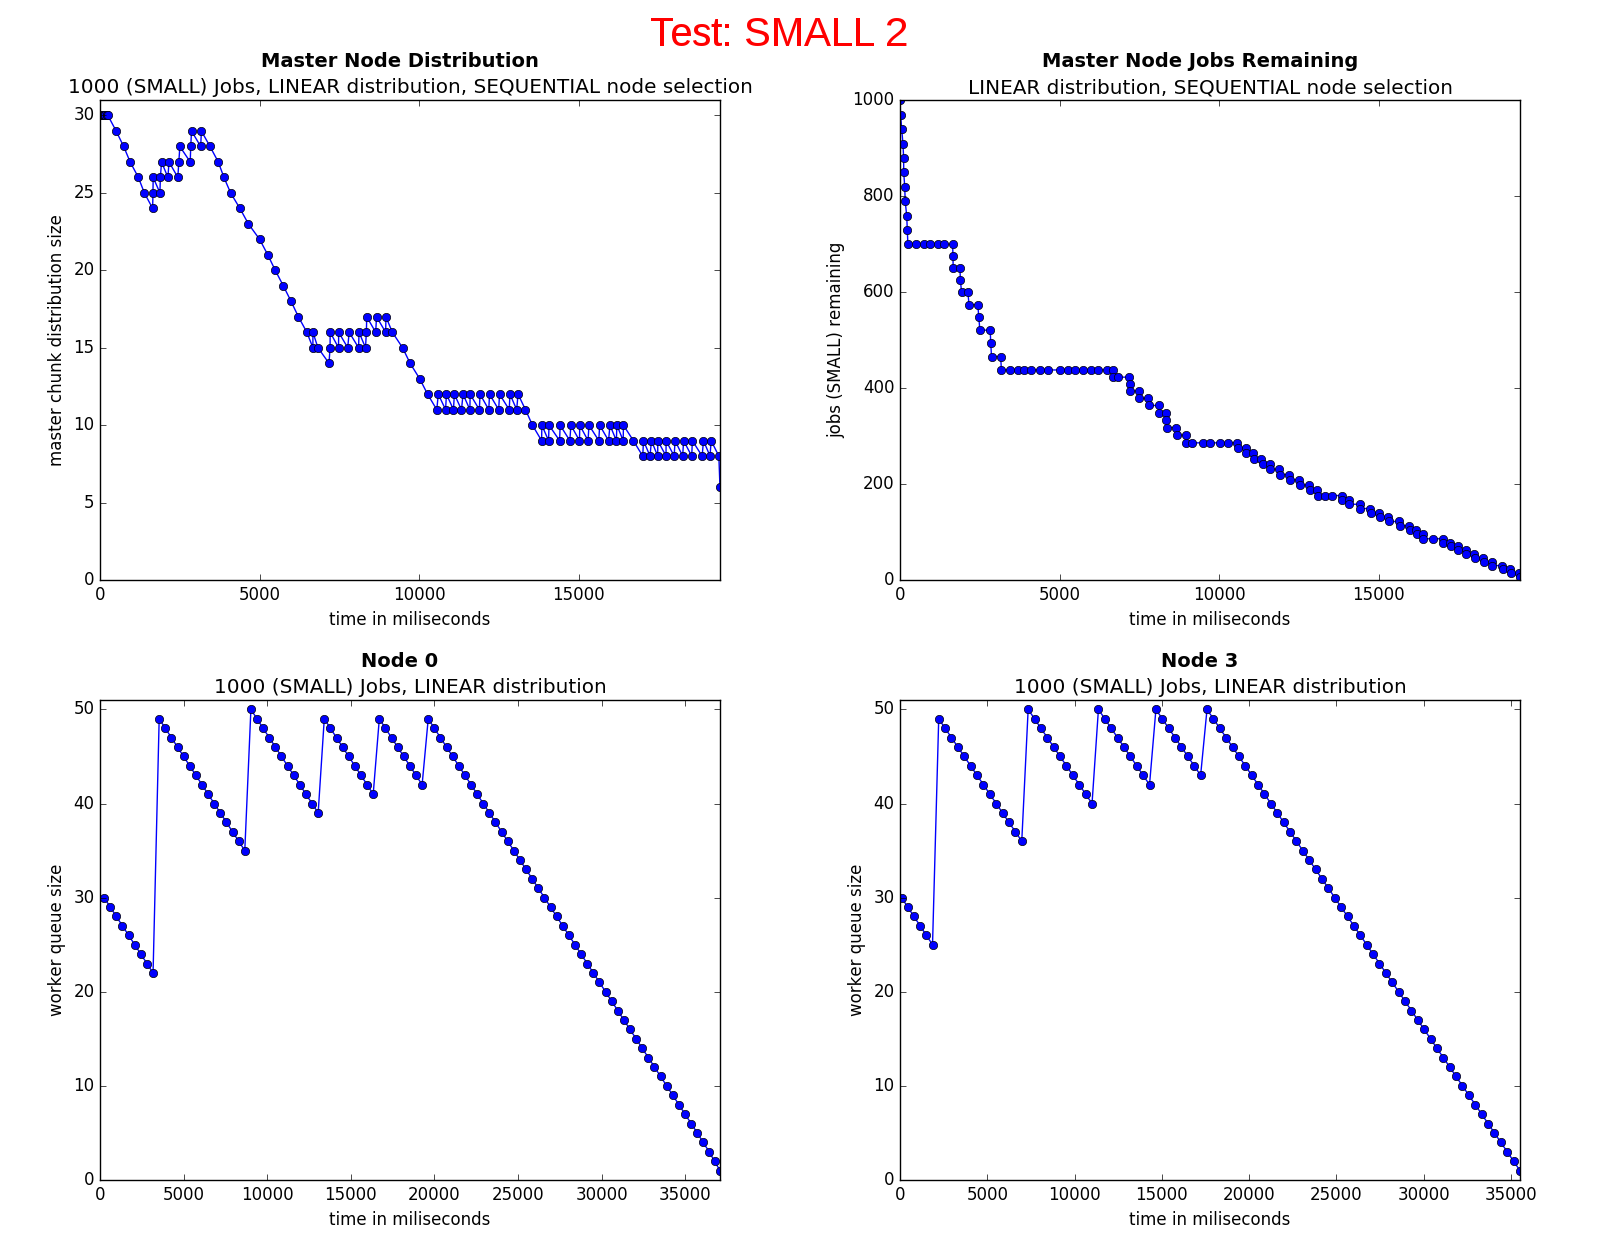
\includegraphics[width=1.2\linewidth]{combined_small_growing_workers_linear/case_small_2} 
    \caption{10 workers} 
    \label{testLinearSmall10} 
    \vspace{4ex}
  \end{subfigure} 
  
  
  \begin{subfigure}[b]{0.5\linewidth}
    \centering
    \hbox{\hspace{-5.0em} 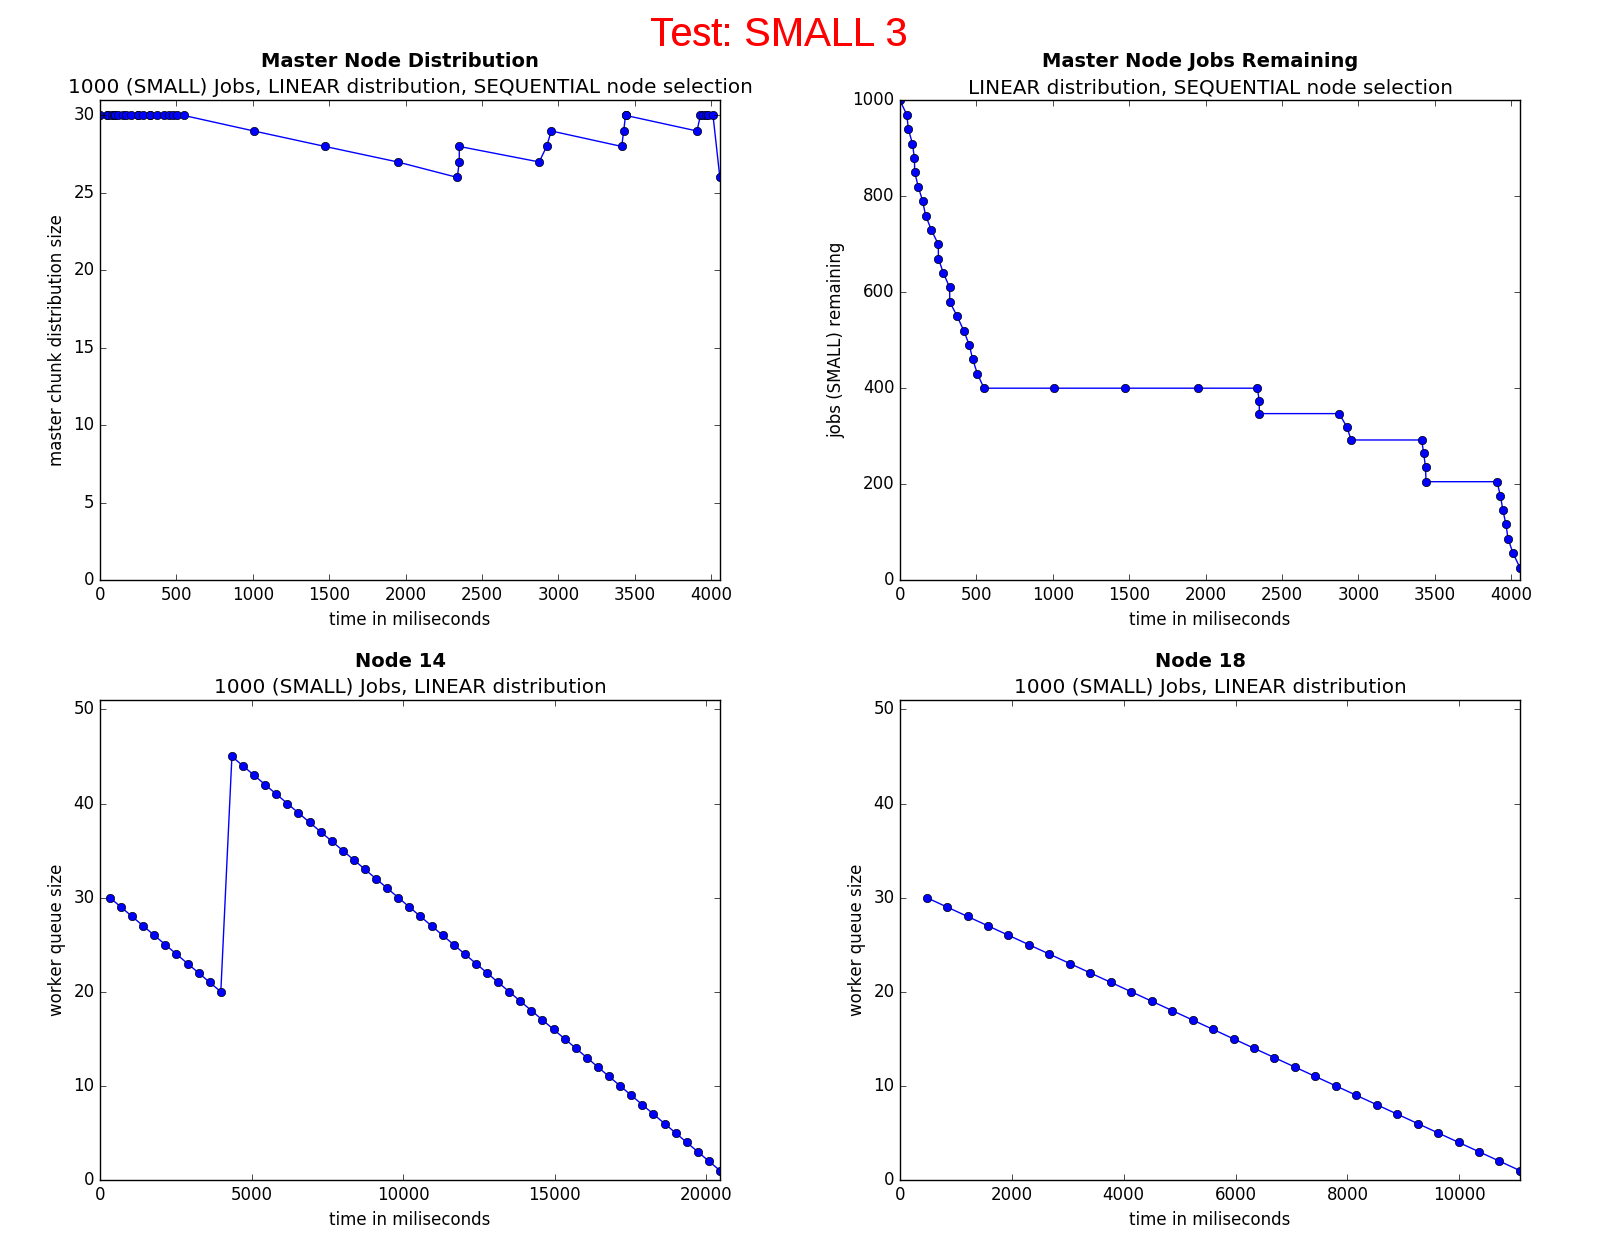
\includegraphics[width=1.2\linewidth]{combined_small_growing_workers_linear/case_small_3} }
    \caption{20 workers} 
    \label{testLinearSmall20} 
    \vspace{4ex}
  \end{subfigure}%% 
  \begin{subfigure}[b]{0.5\linewidth}
    \centering
    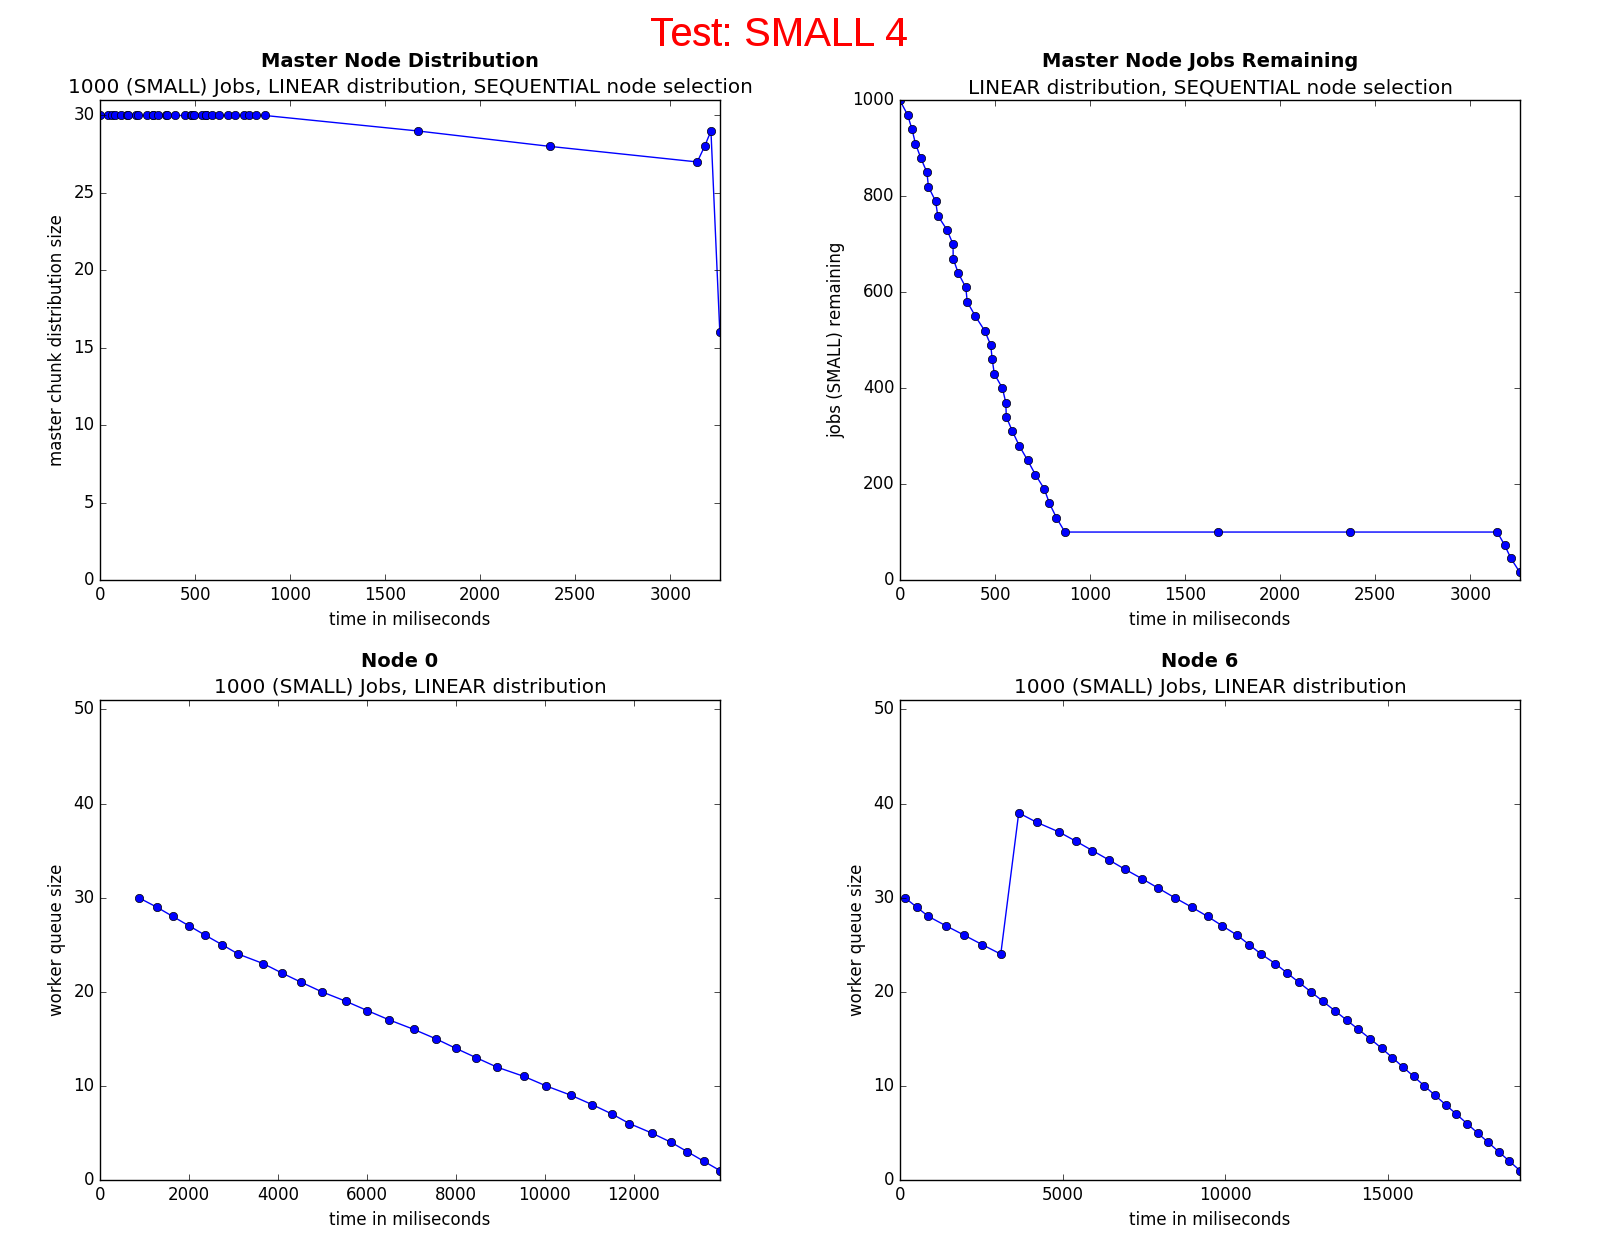
\includegraphics[width=1.2\linewidth]{combined_small_growing_workers_linear/case_small_4} 
    \caption{30 workers} 
    \label{testLinearSmall30} 
    \vspace{4ex}
  \end{subfigure} 
  
  
  \caption{These tests focus on linear job chunk distribution with 1000 small jobs to process and varying worker size. The figures plot results for the small test numbers 1, 2, 3, 4 as labeled at the top of each figure. The top left plot in each figure shows the master job distribution rate as time progresses. The top right plot in each figure shows the number of jobs remaining to distribute as time progresses. The bottom plots in each figure show queue sizes of two randomly selected workers. }
  \label{testsSmallLinear} 
  
\end{figure}
%============================== END SMALL Linear FIGURES
%=================================================



%============================== START SMALL Constant FIGURES
%=================================================
\begin{figure}[p] 
  \begin{subfigure}[b]{0.5\linewidth}
    \centering
    \hbox{\hspace{-5.0em} 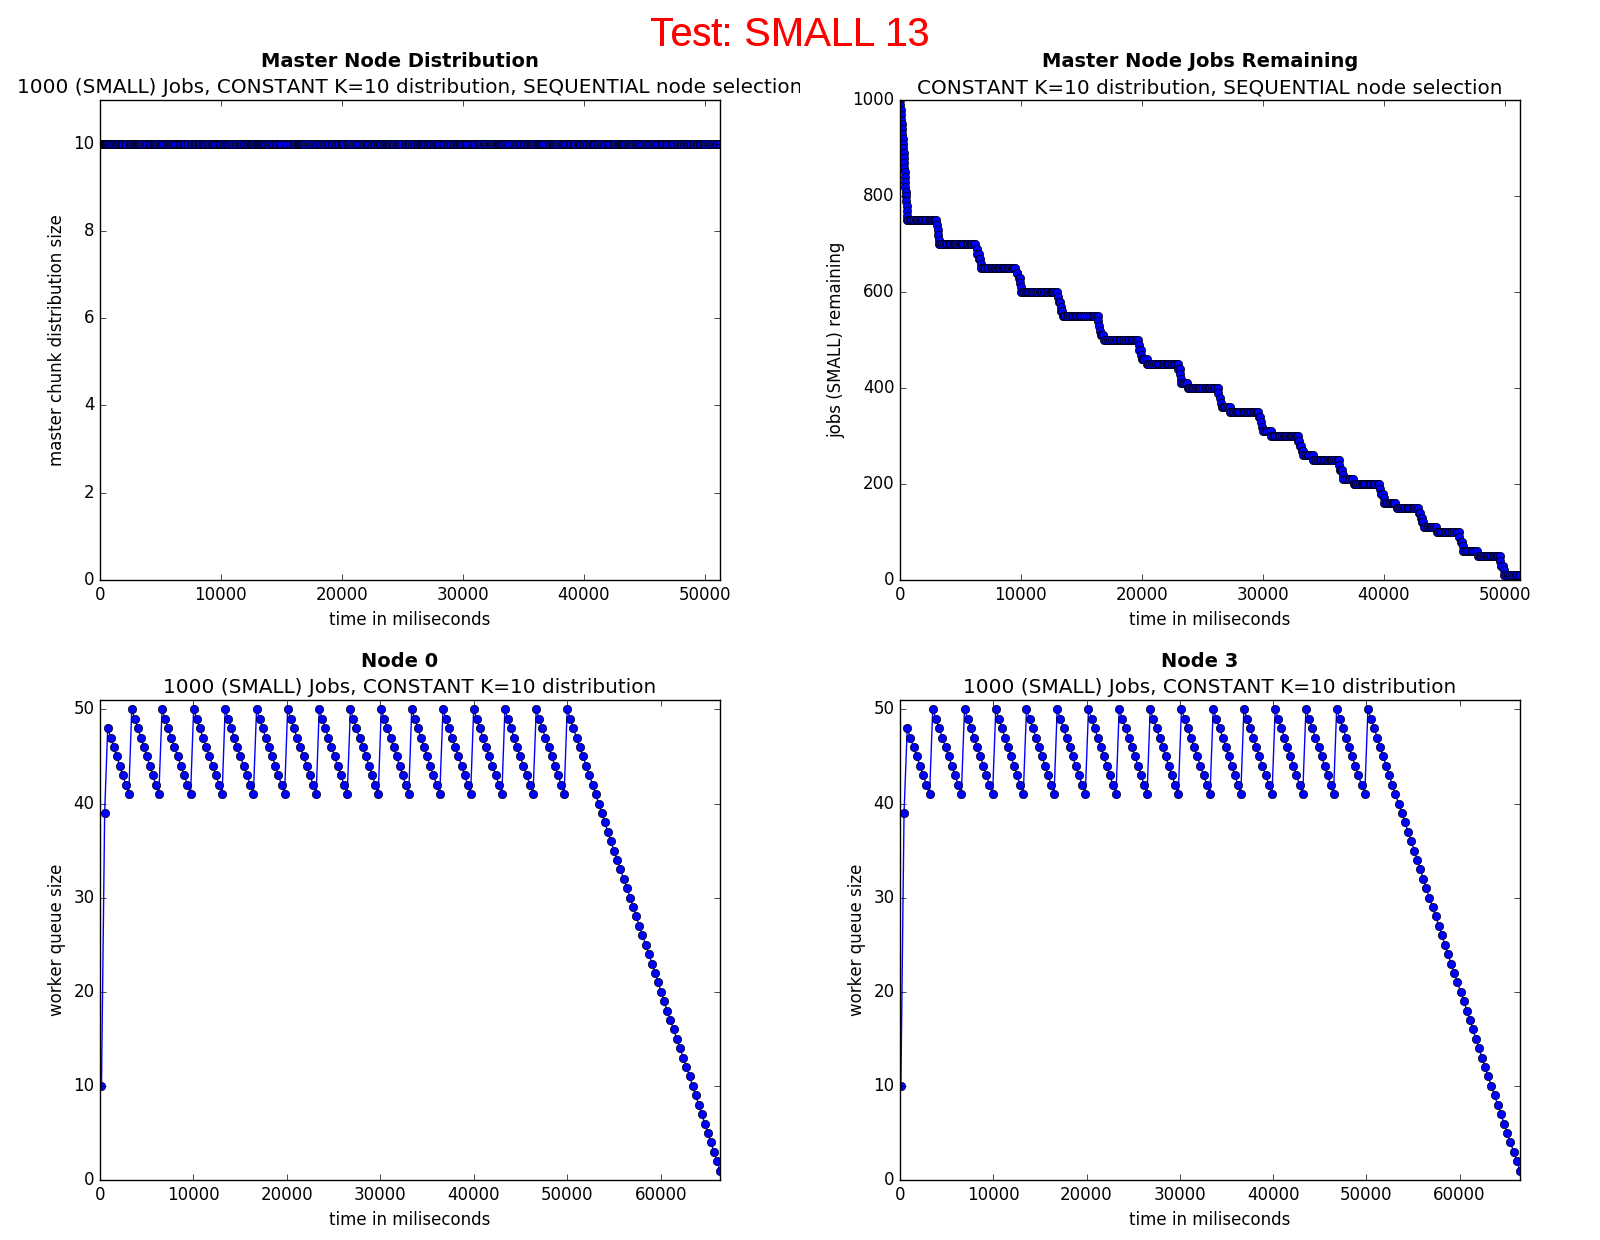
\includegraphics[width=1.2\linewidth]{combined_small_growing_workers_constant/case_small_13} }
    \caption{5 workers}
    \label{testConstantSmall5} 
    \vspace{4ex}
  \end{subfigure}%% 
  \begin{subfigure}[b]{0.5\linewidth}
    \centering
    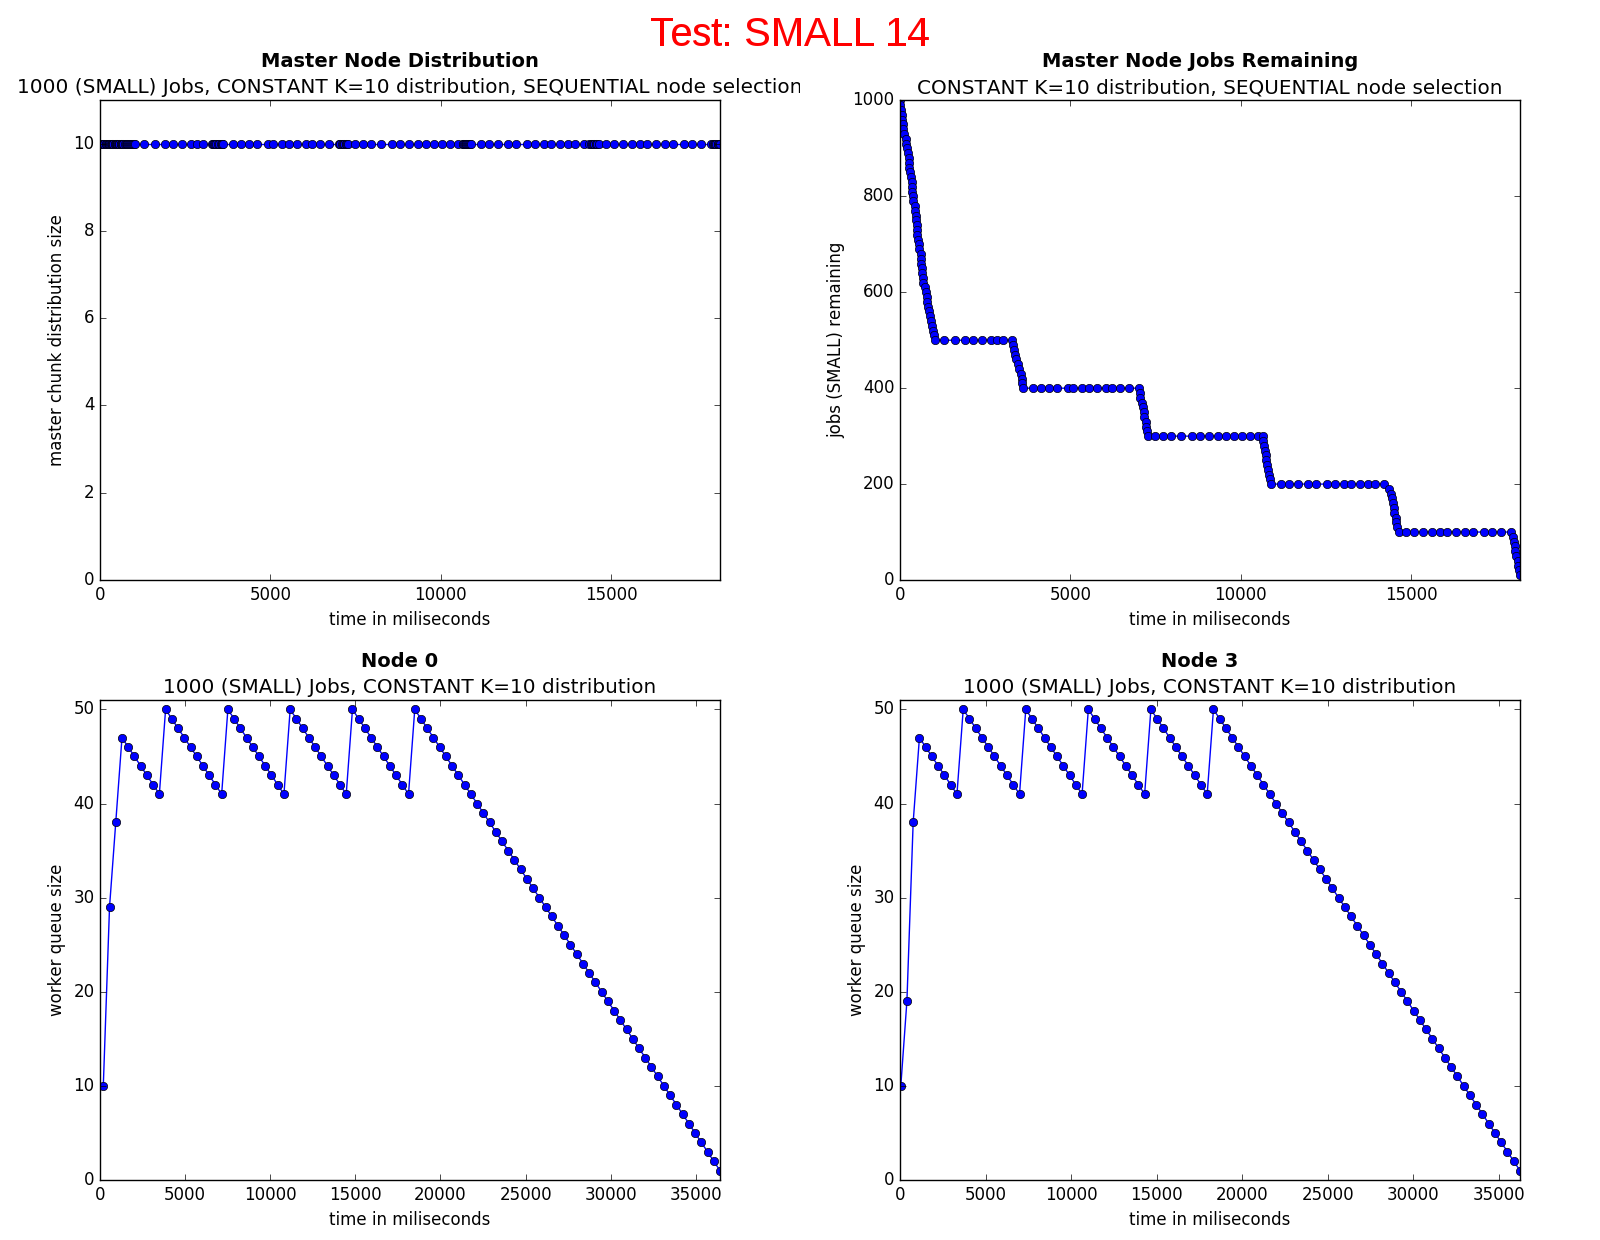
\includegraphics[width=1.2\linewidth]{combined_small_growing_workers_constant/case_small_14} 
    \caption{10 workers} 
    \label{testConstantSmall10} 
    \vspace{4ex}
  \end{subfigure} 
  
  
  \begin{subfigure}[b]{0.5\linewidth}
    \centering
    \hbox{\hspace{-5.0em} 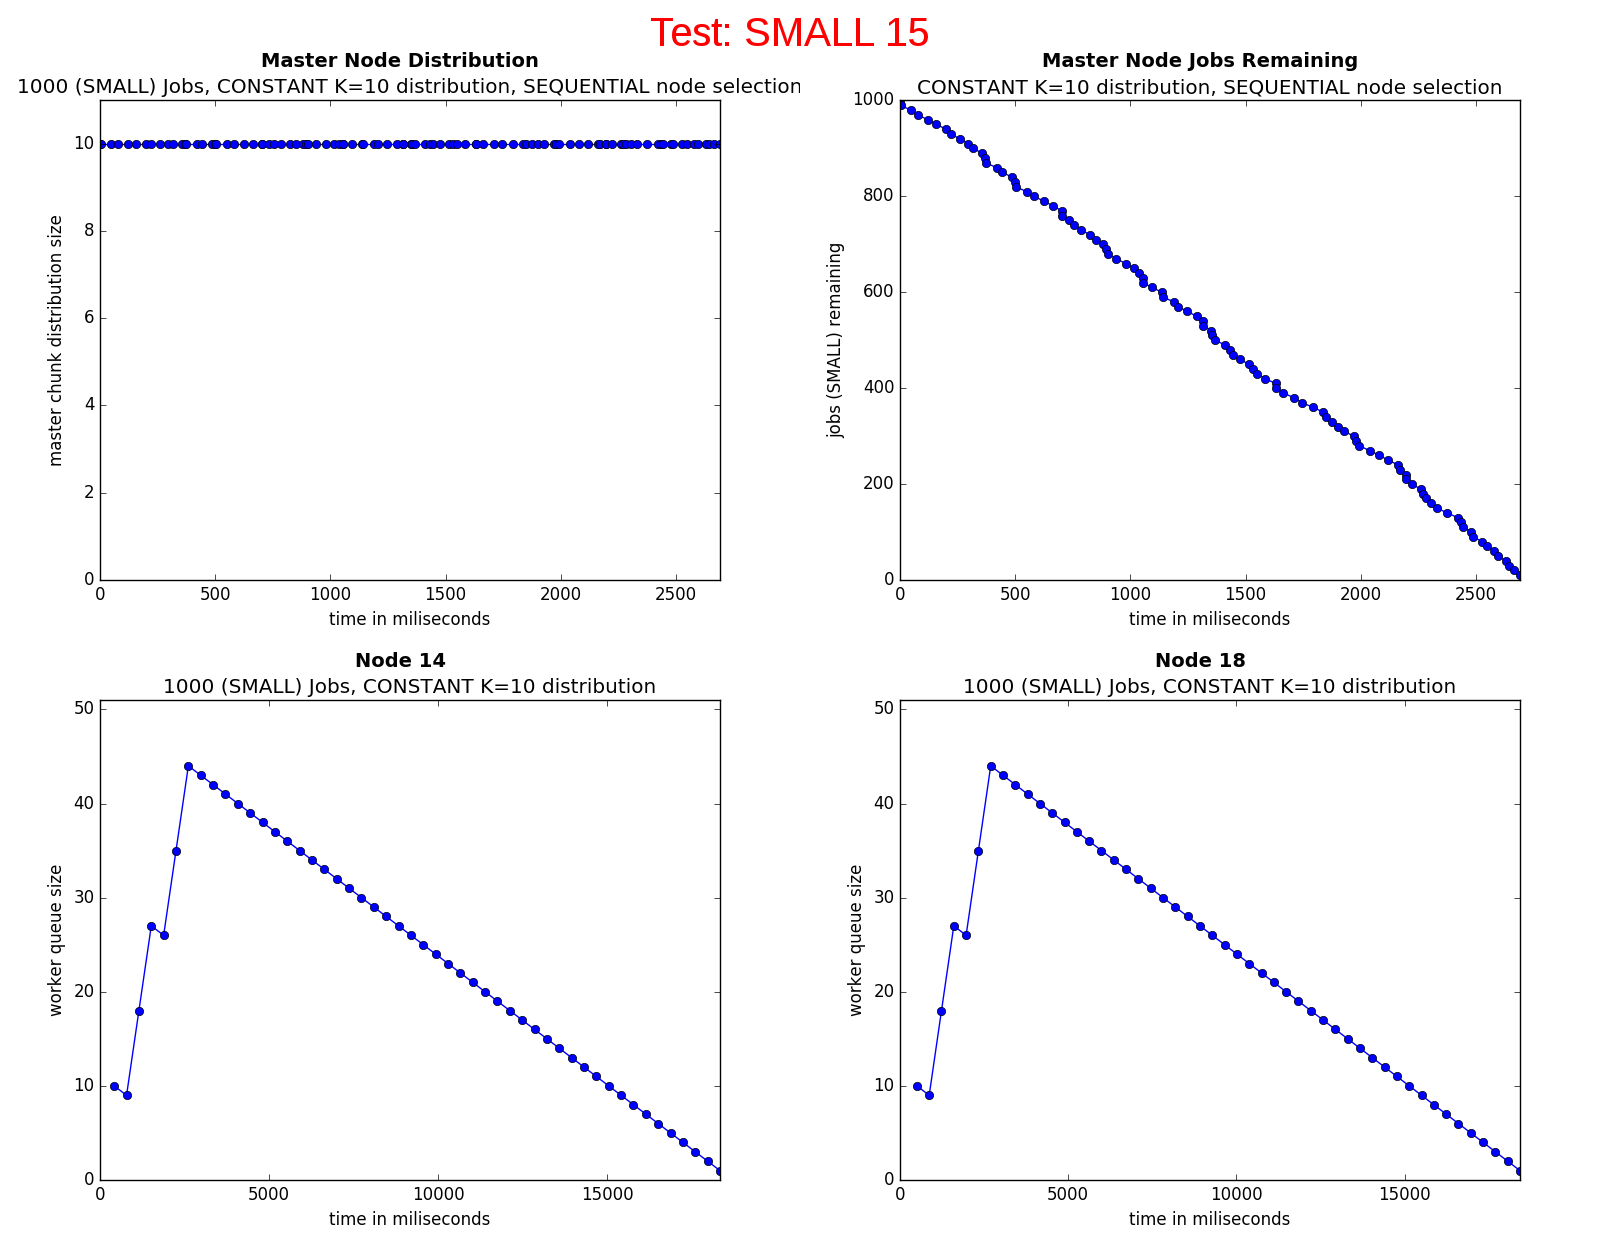
\includegraphics[width=1.2\linewidth]{combined_small_growing_workers_constant/case_small_15} }
    \caption{20 workers} 
    \label{testConstantSmall20} 
    \vspace{4ex}
  \end{subfigure}%% 
  \begin{subfigure}[b]{0.5\linewidth}
    \centering
    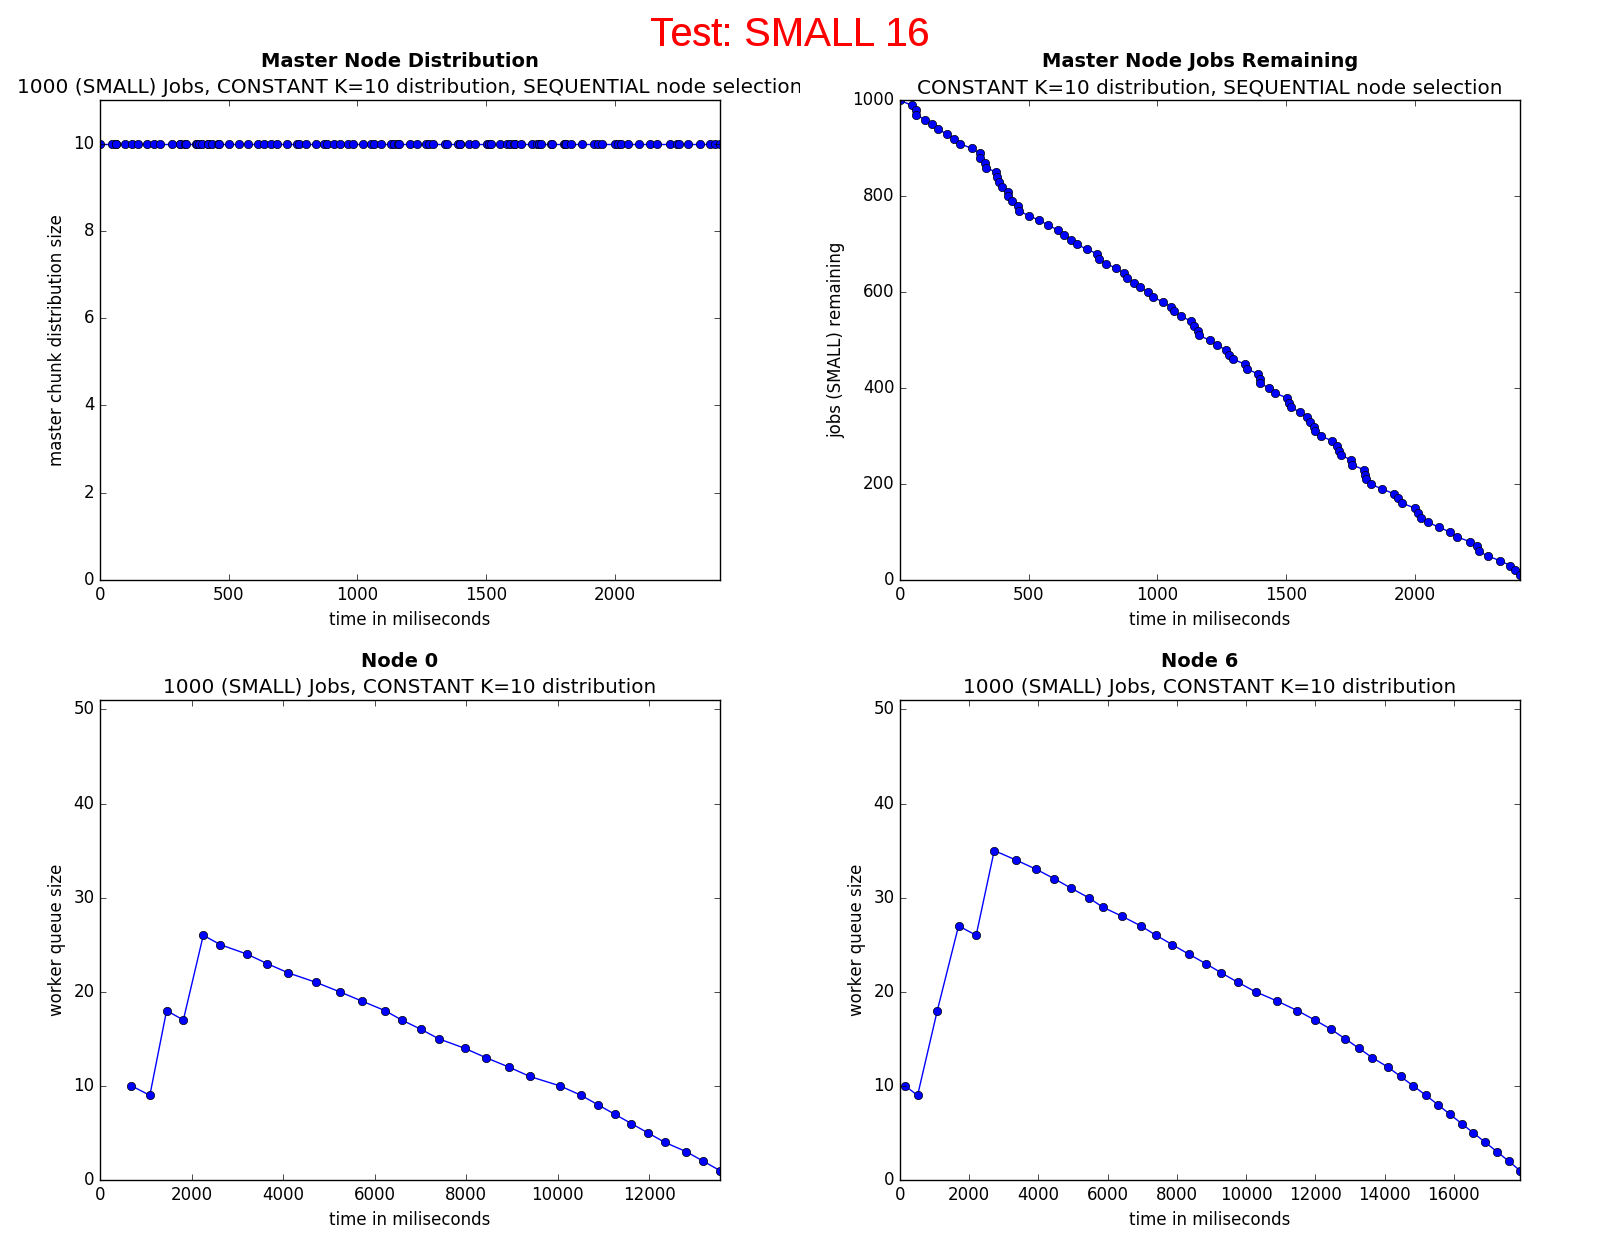
\includegraphics[width=1.2\linewidth]{combined_small_growing_workers_constant/case_small_16} 
    \caption{30 workers} 
    \label{testConstantSmall30} 
    \vspace{4ex}
  \end{subfigure} 
  
  
  \caption{These tests focus on constant job chunk distribution with 1000 small jobs to process and varying worker size. The figures plot results for the small test numbers 13, 14, 15, 16 as labeled at the top of each figure. The top left plot in each figure shows the master job distribution rate as time progresses. The top right plot in each figure shows the number of jobs remaining to distribute as time progresses. The bottom plots in each figure show queue sizes of two randomly selected workers.}
  \label{testsSmallConstant} 
  
\end{figure}
%============================== END SMALL Constant FIGURES
%=================================================

\newpage

% OK
\section{Results: 1000 Varied Jobs} \label{1000VariedJobs}
Table \ref{variedJobsTable} shows all the test configurations for 1000 varied jobs. The last two columns specify the execution time as well as the estimated sequential execution time. Figures \ref{testVaried1-13}, \ref{testsVaried17-29}, \ref{testVaried33Figure} show an overview of results where 5 worker nodes were used.

% OK
\subsection{Varying Node Selection} \label{variedNodeSelection}
Similarly as in small job type, node selection does not seem to have much of an effect on the plots. This can be inspected in Figures \ref{testVaried1}, \ref{testVaried5}, \ref{testVaried9} where job distribution is linear while node selection is varied. Although, the same conclusion can be reached regarding random node selection performing worse than others when inspecting Table \ref{variedJobsTable}. In this instance, random performs equal or on average about 1.5 seconds worse than the other two strategies.

% OK
\subsection{Varying Job Distribution Strategy} \label{variedJobDistribution}
Similarly, as in Section \ref{variedJobDistribution}, inspecting the time in Table \ref{variedJobsTable} shows that constant distribution strategy performs around 1 second better than the other two strategies.

Additionally, as the number of workers grow, the job chunk size variation does not decrease as much as it did with 1000 small jobs. For instance in Figure \ref{testLinearVaried10} job chunk size goes from around 30 jobs to around 5-4 jobs. While in the small jobs case Figure \ref{testLinearSmall10} goes from around 30 jobs to around 10 jobs. This means that for varied workloads, linear and exponential distribution strategies are more likely to spread the job load evenly when the number of workers is small.

% OK
\subsubsection{Linear Job Distribution} \label{variedJobDistributionLinear}
In general patterns occurring in Section \ref{smallJobDistributionLinear} for workloads composed of small jobs subjected to a linear job distribution also occurred for workloads composed of varied jobs subjected to a linear job distribution. This can be seen in Figure \ref{testsVariedLinear}.

% OK
\subsubsection{Exponential Job Distribution} \label{variedJobDistributionExp}
It is interesting to note that the master job chunk size is much less likely to return to the maximum value in the varied case. In Figure \ref{testExpSmall10} the rate can be observed on two occasions to nearly reach the 30 maximum job chunk size, while in Figure \ref{testExpVaried10} the job chunk size after a certain time does not go beyond 15.

% OK
\subsubsection{Constant Job Distribution} \label{variedJobDistributionConstant}
In the varied case, the plots in top right of Figures \ref{testConstantVaried20}, \ref{testConstantVaried30} showing the number of jobs left, are not displaying as much of a stepwise descent as they did in the case of small jobs. The variation in jobs must have allowed the master node to distribute a bit better.


%============================ START VARIED TABLE RESULTS
%=================================================
\begin{table}

\hspace*{-4em}
\begin{tabular}{|c | c | c | c | c | c | c |}
\hline
\textbf{Test \#} & \textbf{Job Number} & \textbf{\# of Workers} & \textbf{Node} & \textbf{Distribution} & \textbf{Execution} & \textbf{Sequential} \\

 & \textbf{\& Size} &  & \textbf{Selection} &  & \textbf{Time (sec)} & \textbf{Time (sec)} \\

\hline
1  & 1000 VARIED JOBS & 5  & SEQUENTIAL & LINEAR            & 161.844156 & 754.053213 \\ \hline
2  & 1000 VARIED JOBS & 10 & SEQUENTIAL & LINEAR            & 89.742808  & 738.409125 \\ \hline
3  & 1000 VARIED JOBS & 20 & SEQUENTIAL & LINEAR            & 53.982696  & 736.704731 \\ \hline
4  & 1000 VARIED JOBS & 30 & SEQUENTIAL & LINEAR            & 54.338283  & 751.345197 \\ \hline
   &                  &    &            &                   &            &            \\ \hline
5  & 1000 VARIED JOBS & 5  & RANDOM     & LINEAR            & 158.770141 & 753.83557  \\ \hline
6  & 1000 VARIED JOBS & 10 & RANDOM     & LINEAR            & 91.350818  & 738.928114 \\ \hline
7  & 1000 VARIED JOBS & 20 & RANDOM     & LINEAR            & 53.600079  & 747.684029 \\ \hline
8  & 1000 VARIED JOBS & 30 & RANDOM     & LINEAR            & 51.587202  & 753.658543 \\ \hline
   &                  &    &            &                   &            &            \\ \hline
9  & 1000 VARIED JOBS & 5  & SQS        & LINEAR            & 158.538569 & 743.892494 \\ \hline
10 & 1000 VARIED JOBS & 10 & SQS        & LINEAR            & 89.631225  & 732.140331 \\ \hline
11 & 1000 VARIED JOBS & 20 & SQS        & LINEAR            & 55.47384   & 755.899796 \\ \hline
12 & 1000 VARIED JOBS & 30 & SQS        & LINEAR            & 48.615173  & 754.232638 \\ \hline
   &                  &    &            &                   &            &            \\ \hline
13 & 1000 VARIED JOBS & 5  & SEQUENTIAL & CONSTANT (K = 10) & 159.512476 & 745.68618  \\ \hline
14 & 1000 VARIED JOBS & 10 & SEQUENTIAL & CONSTANT (K = 10) & 91.318658  & 747.735918 \\ \hline
15 & 1000 VARIED JOBS & 20 & SEQUENTIAL & CONSTANT (K = 10) & 46.774289  & 749.278662 \\ \hline
16 & 1000 VARIED JOBS & 30 & SEQUENTIAL & CONSTANT (K = 10) & 40.697084  & 731.82836  \\ \hline
   &                  &    &            &                   &            &            \\ \hline
17 & 1000 VARIED JOBS & 5  & RANDOM     & CONSTANT (K = 10) & 162.045801 & 755.382666 \\ \hline
18 & 1000 VARIED JOBS & 10 & RANDOM     & CONSTANT (K = 10) & 93.745082  & 753.163448 \\ \hline
19 & 1000 VARIED JOBS & 20 & RANDOM     & CONSTANT (K = 10) & 51.682266  & 780.054384 \\ \hline
20 & 1000 VARIED JOBS & 30 & RANDOM     & CONSTANT (K = 10) & 49.178355  & 738.993456 \\ \hline
   &                  &    &            &                   &            &            \\ \hline
21 & 1000 VARIED JOBS & 5  & SQS        & CONSTANT (K = 10) & 155.964292 & 733.491056 \\ \hline
22 & 1000 VARIED JOBS & 10 & SQS        & CONSTANT (K = 10) & 89.77435   & 736.275724 \\ \hline
23 & 1000 VARIED JOBS & 20 & SQS        & CONSTANT (K = 10) & 48.082729  & 736.751697 \\ \hline
24 & 1000 VARIED JOBS & 30 & SQS        & CONSTANT (K = 10) & 41.264443  & 745.566809 \\ \hline
   &                  &    &            &                   &            &            \\ \hline
25 & 1000 VARIED JOBS & 5  & SEQUENTIAL & EXP               & 155.947948 & 737.656006 \\ \hline
26 & 1000 VARIED JOBS & 10 & SEQUENTIAL & EXP               & 87.764681  & 741.957524 \\ \hline
27 & 1000 VARIED JOBS & 20 & SEQUENTIAL & EXP               & 56.013402  & 739.046668 \\ \hline
28 & 1000 VARIED JOBS & 30 & SEQUENTIAL & EXP               & 48.870783  & 738.489488 \\ \hline
   &                  &    &            &                   &            &            \\ \hline
29 & 1000 VARIED JOBS & 5  & RANDOM     & EXP               & 162.617345 & 743.977726 \\ \hline
30 & 1000 VARIED JOBS & 10 & RANDOM     & EXP               & 91.397033  & 746.30314  \\ \hline
31 & 1000 VARIED JOBS & 20 & RANDOM     & EXP               & 55.964803  & 742.597571 \\ \hline
32 & 1000 VARIED JOBS & 30 & RANDOM     & EXP               & 50.481499  & 762.706475 \\ \hline
   &                  &    &            &                   &            &            \\ \hline
33 & 1000 VARIED JOBS & 5  & SQS        & EXP               & 161.504917 & 745.572964 \\ \hline
34 & 1000 VARIED JOBS & 10 & SQS        & EXP               & 91.471311  & 764.73493  \\ \hline
35 & 1000 VARIED JOBS & 20 & SQS        & EXP               & 51.42736   & 745.500791 \\ \hline
36 & 1000 VARIED JOBS & 30 & SQS        & EXP               & 43.326807  & 738.88087  \\ \hline
\end{tabular}

\caption{Listing of all test cases ran on 1000 varied jobs. \label{variedJobsTable}}
\end{table}
%============================ END VARIED TABLE RESULTS
%=================================================


%============================ START VARIED OverView FIGURES
%=================================================
\begin{figure} 
  \begin{subfigure}[b]{0.5\linewidth}
    \centering
    \hbox{\hspace{-5.0em} \includegraphics[width=1.2\linewidth]{combined_varied_overview/case_varied_1} }
    \caption{Sequential node selection, Linear distribution}
    \label{testVaried1} 
    \vspace{4ex}
  \end{subfigure}%% 
  \begin{subfigure}[b]{0.5\linewidth}
    \centering
    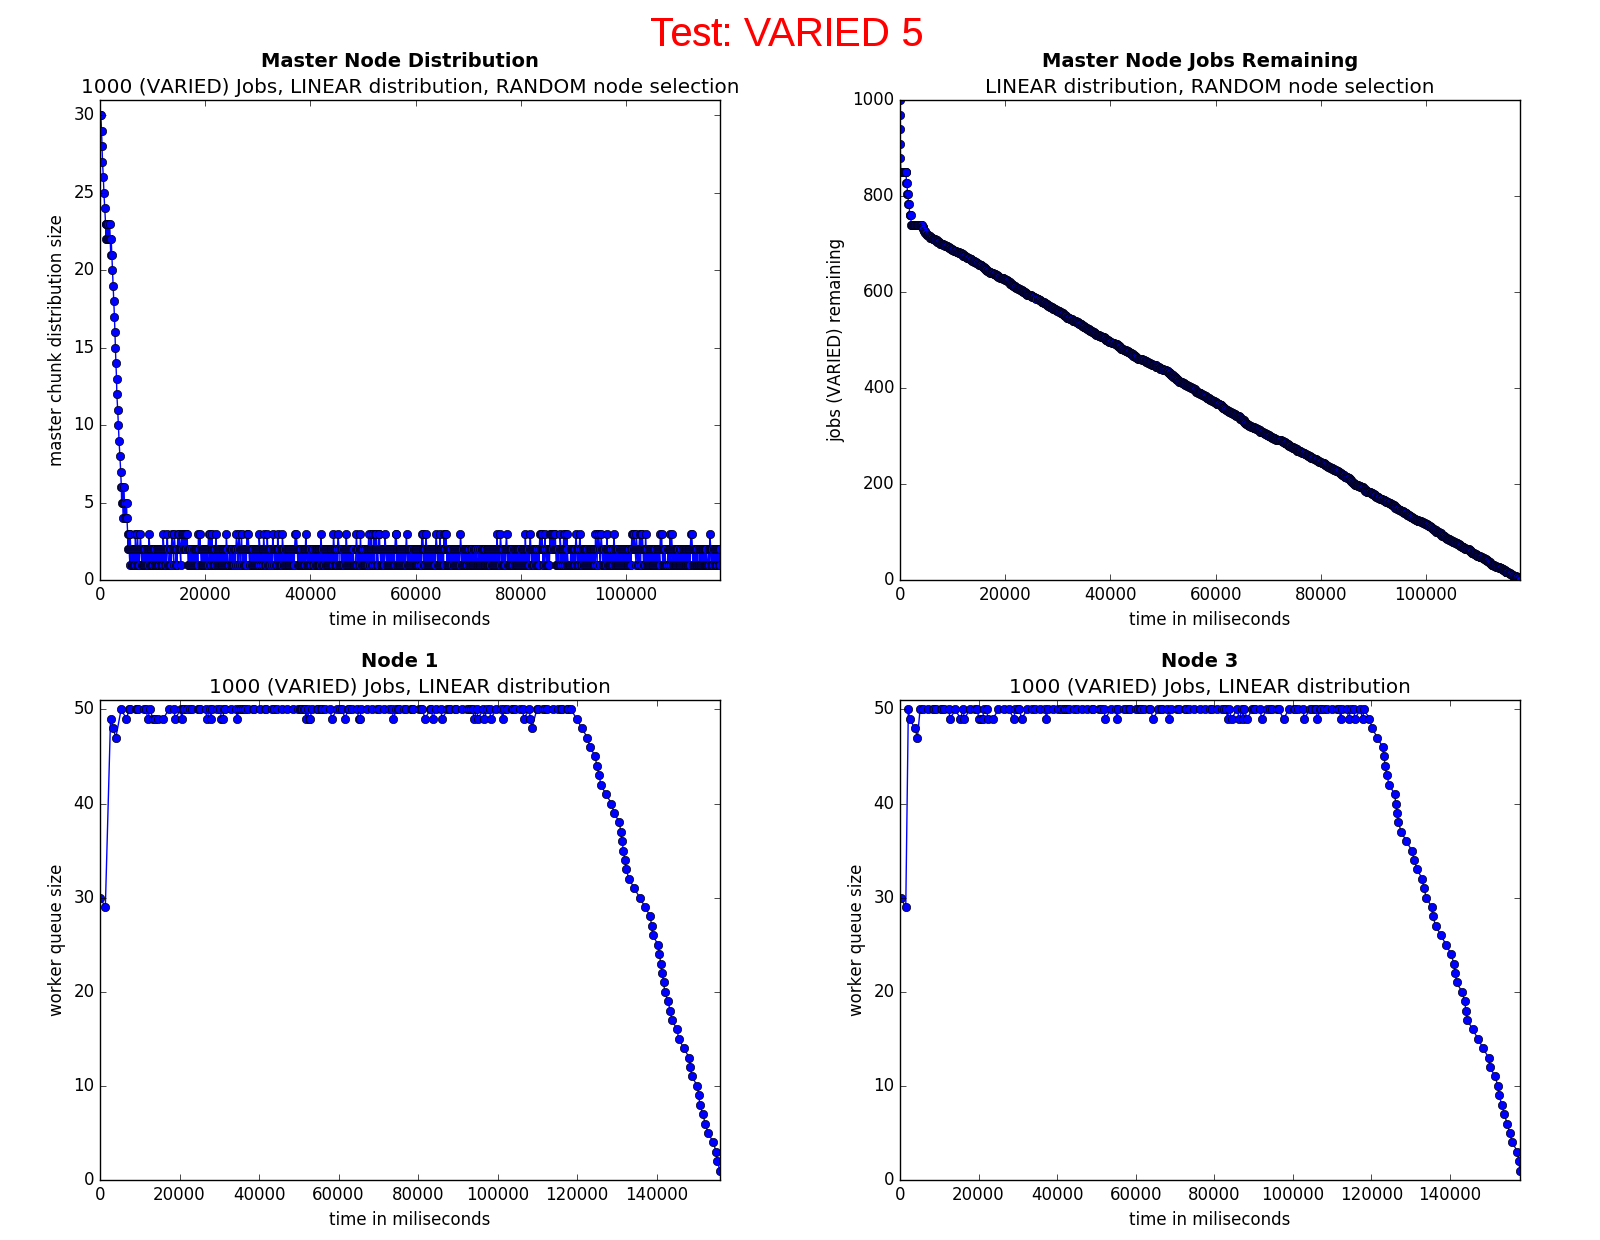
\includegraphics[width=1.2\linewidth]{combined_varied_overview/case_varied_5} 
    \caption{Random node selection, Linear distribution} 
    \label{testVaried5} 
    \vspace{4ex}
  \end{subfigure} 
  
  \begin{subfigure}[b]{0.5\linewidth}
    \centering
    \hbox{\hspace{-5.0em} 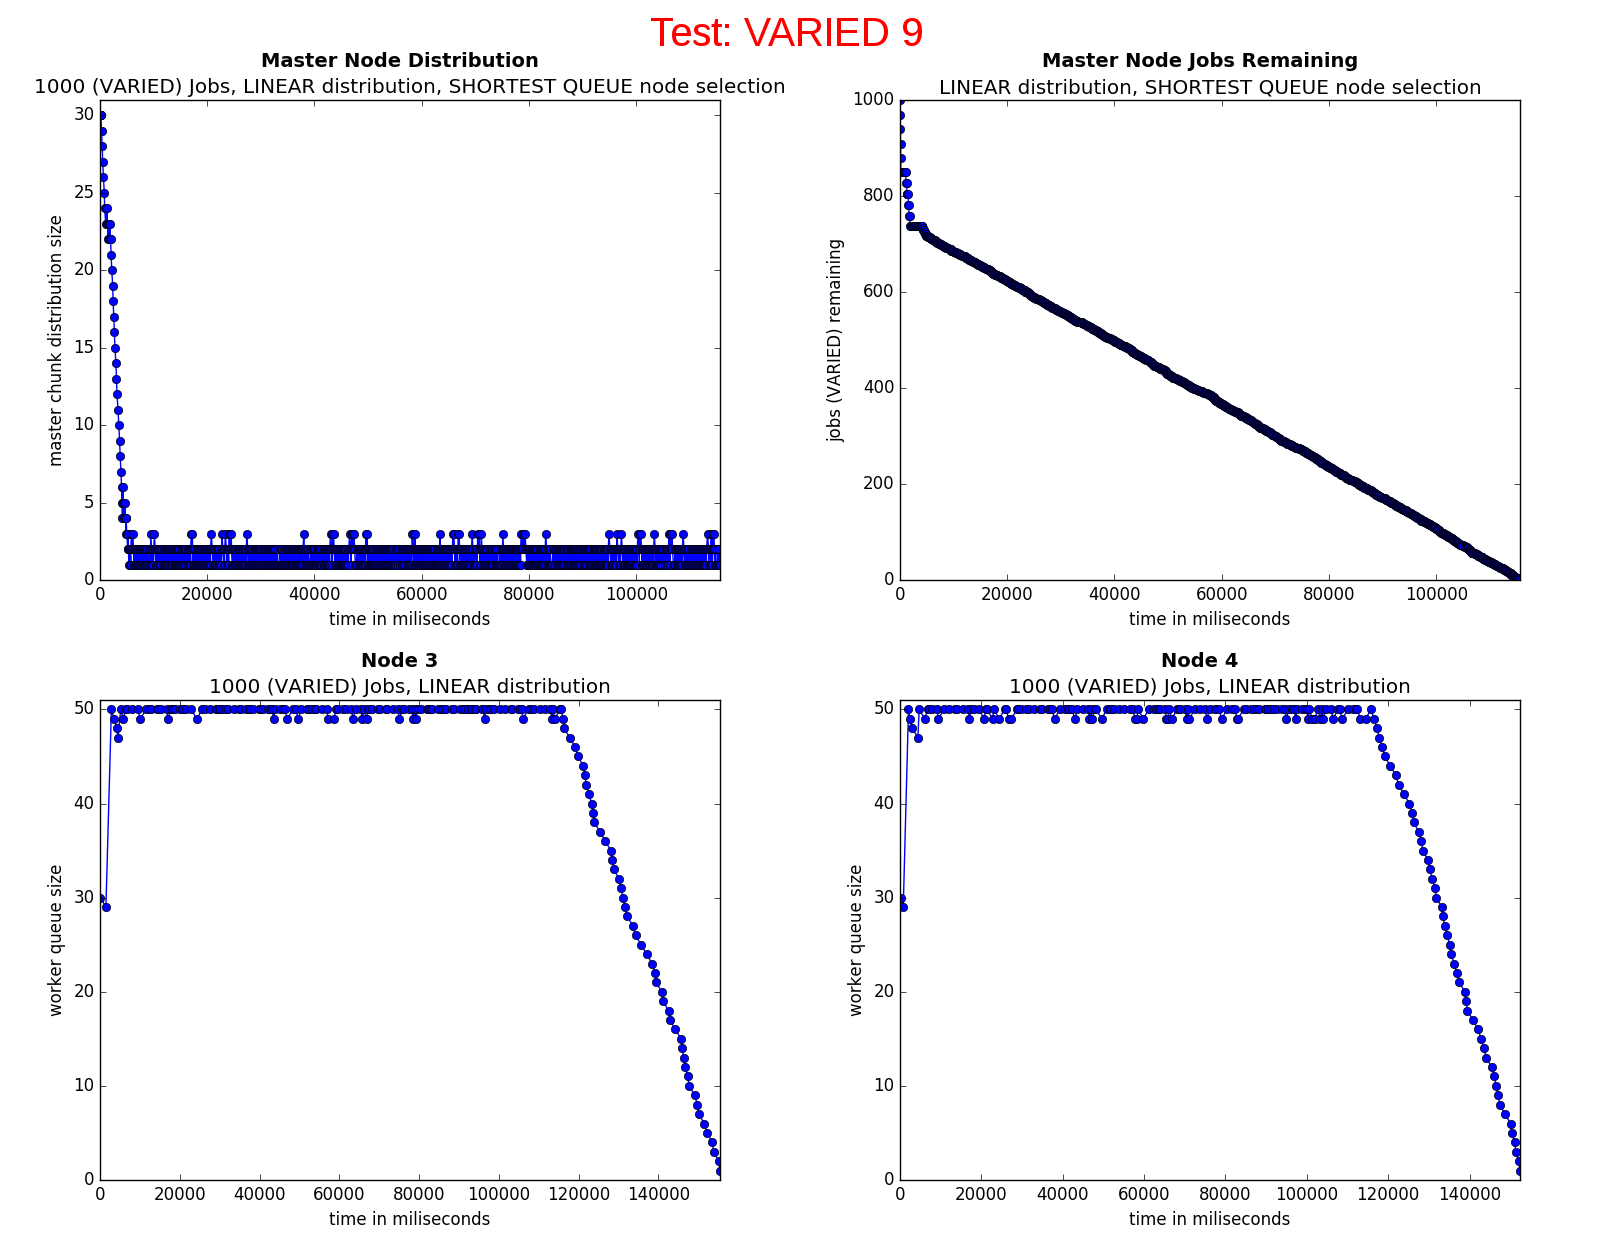
\includegraphics[width=1.2\linewidth]{combined_varied_overview/case_varied_9} }
    \caption{Shortest Queue node selection, Linear distribution} 
    \label{testVaried9} 
    \vspace{4ex}
  \end{subfigure}%% 
  \begin{subfigure}[b]{0.5\linewidth}
    \centering
    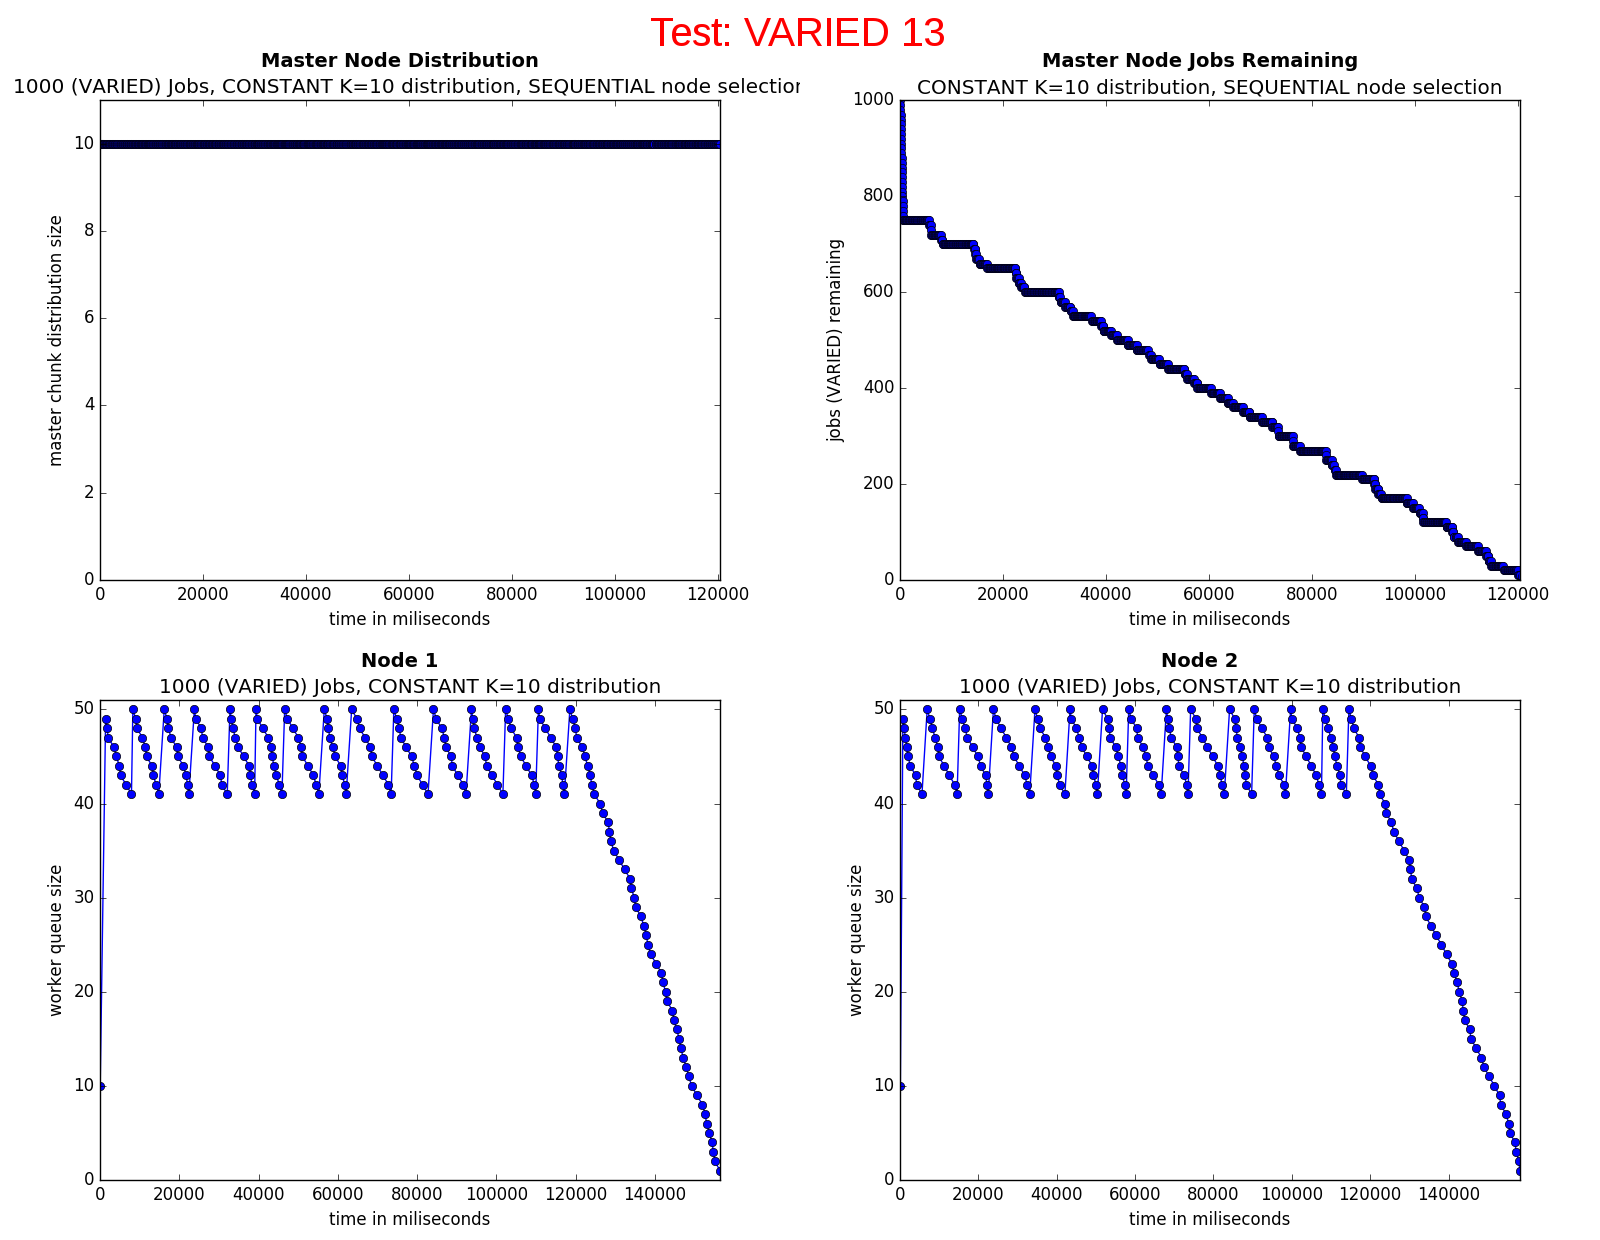
\includegraphics[width=1.2\linewidth]{combined_varied_overview/case_varied_13} 
    \caption{Sequential node selection, Constant distribution} 
    \label{testVaried13} 
    \vspace{4ex}
  \end{subfigure} 
  
  
  \caption{Overview of simulation with 1000 varied jobs and 5 worker nodes part 1. These figures plot results for the varied test numbers 1, 5, 9, 13 as labeled at the top of each figure. The top left plot in each figure shows the master job distribution rate as time progresses. The top right plot in each figure shows the number of jobs remaining to distribute as time progresses. The bottom plots in each figure show queue sizes of two randomly selected workers.}
  \label{testVaried1-13} 
  
\end{figure}

\begin{figure}[p] 
  \begin{subfigure}[b]{0.5\linewidth}
    \centering
    \hbox{\hspace{-5.0em} 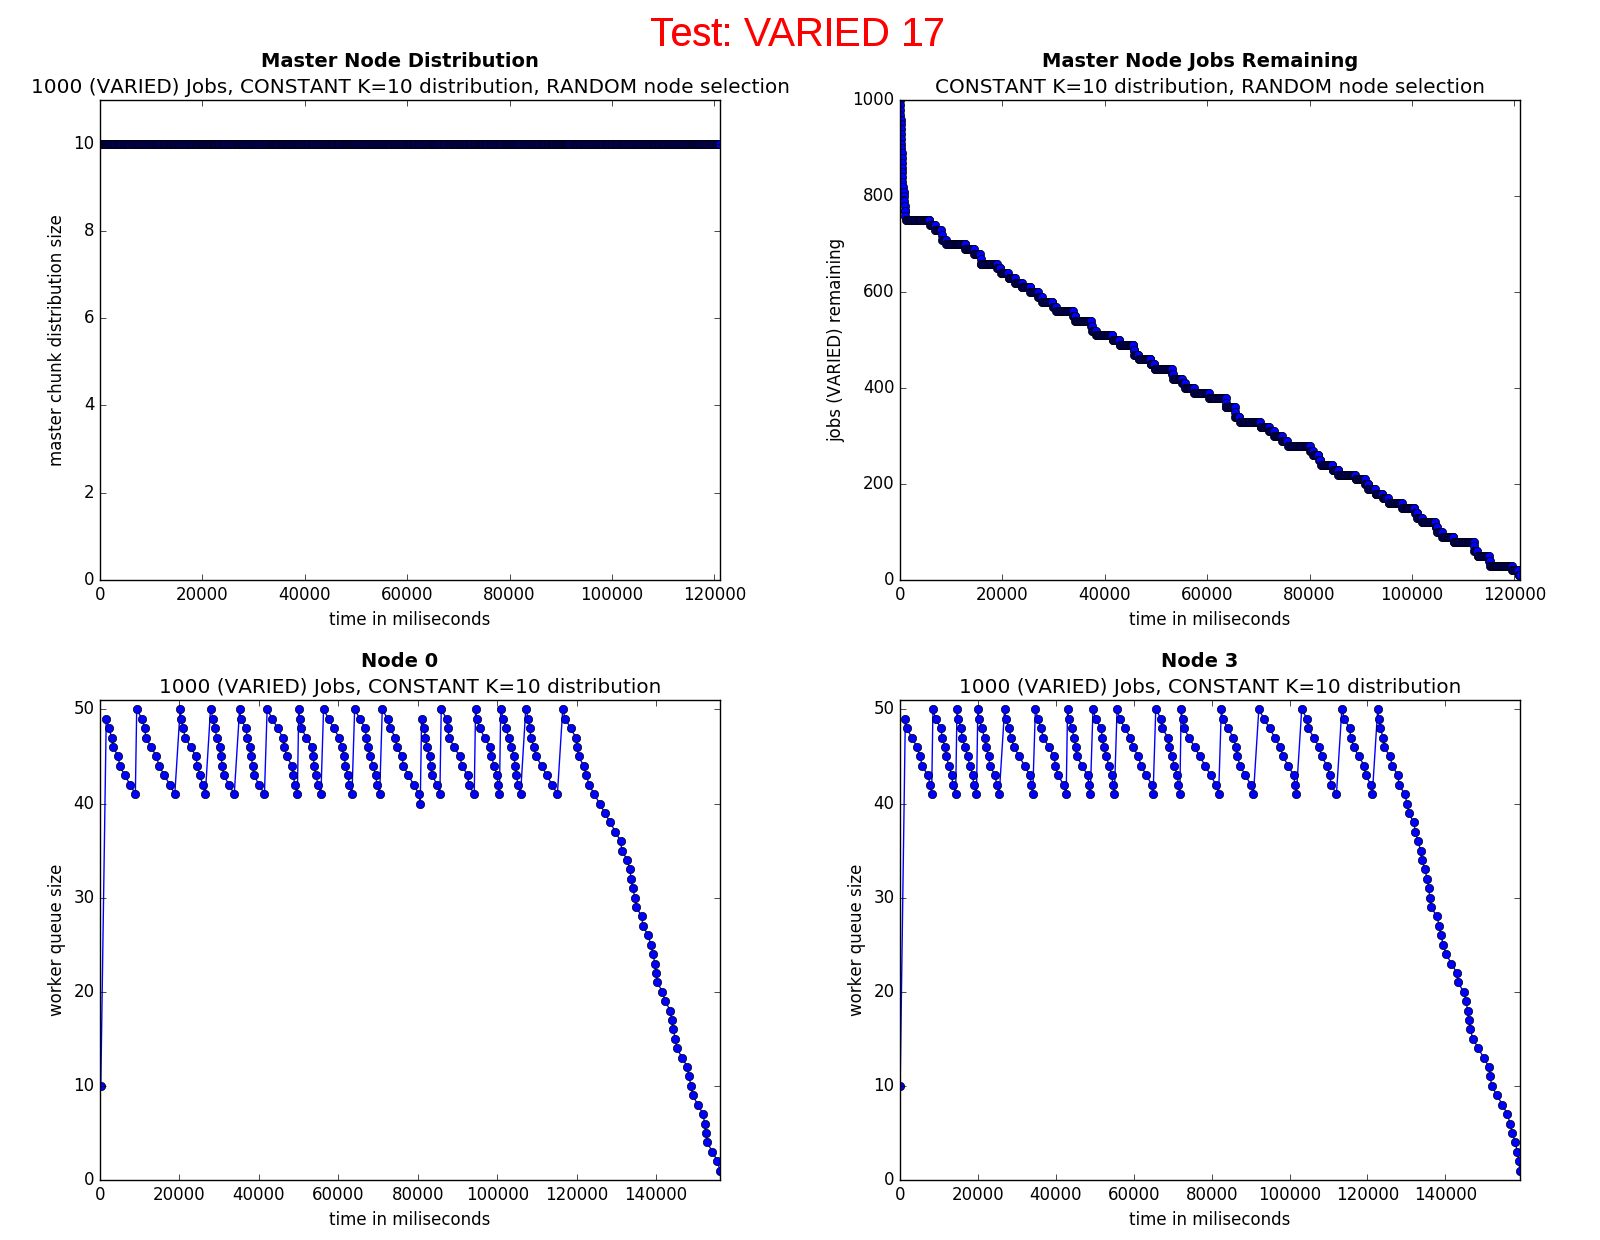
\includegraphics[width=1.2\linewidth]{combined_varied_overview/case_varied_17} }
    \caption{Random node selection, Constant distribution}
    \label{testVaried17} 
    \vspace{4ex}
  \end{subfigure}%% 
  \begin{subfigure}[b]{0.5\linewidth}
    \centering
    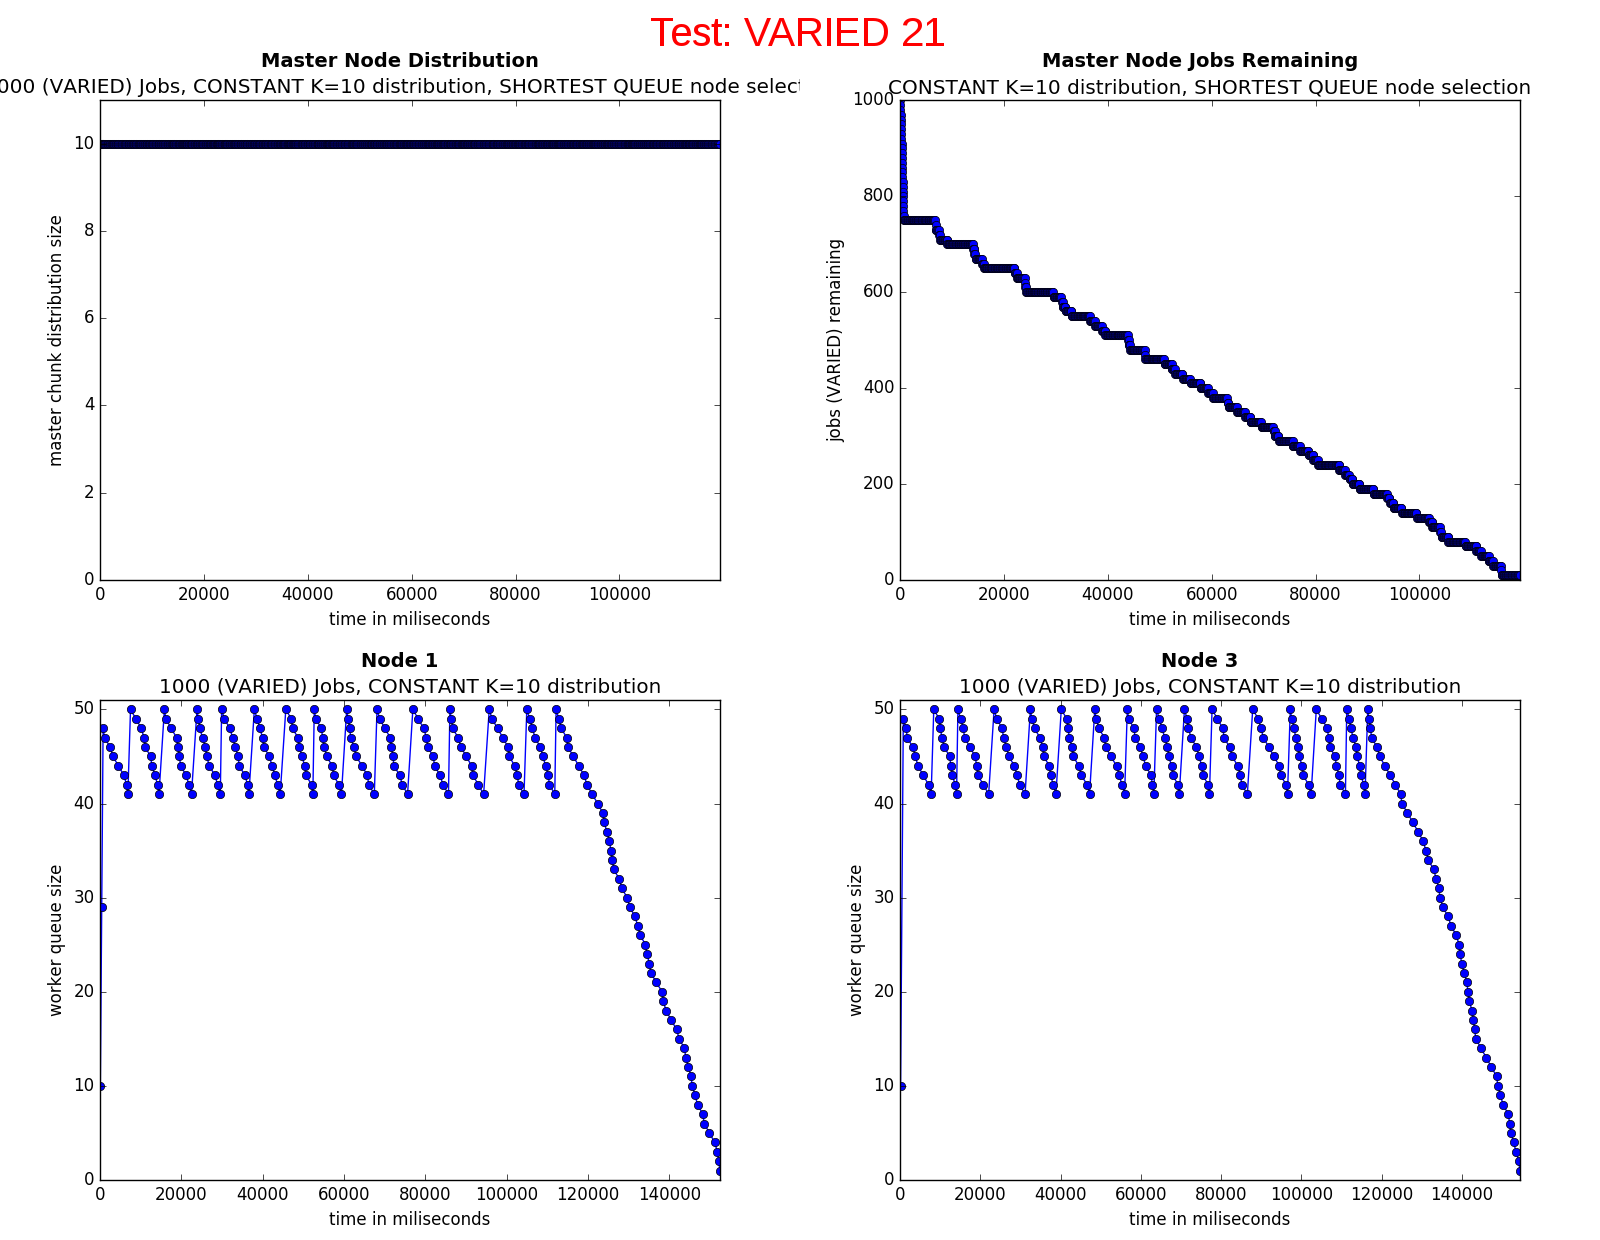
\includegraphics[width=1.2\linewidth]{combined_varied_overview/case_varied_21} 
    \caption{Shortest queue node selection, Constant distribution} 
    \label{testVaried21} 
    \vspace{4ex}
  \end{subfigure} 
  
  
  \begin{subfigure}[b]{0.5\linewidth}
    \centering
    \hbox{\hspace{-5.0em} 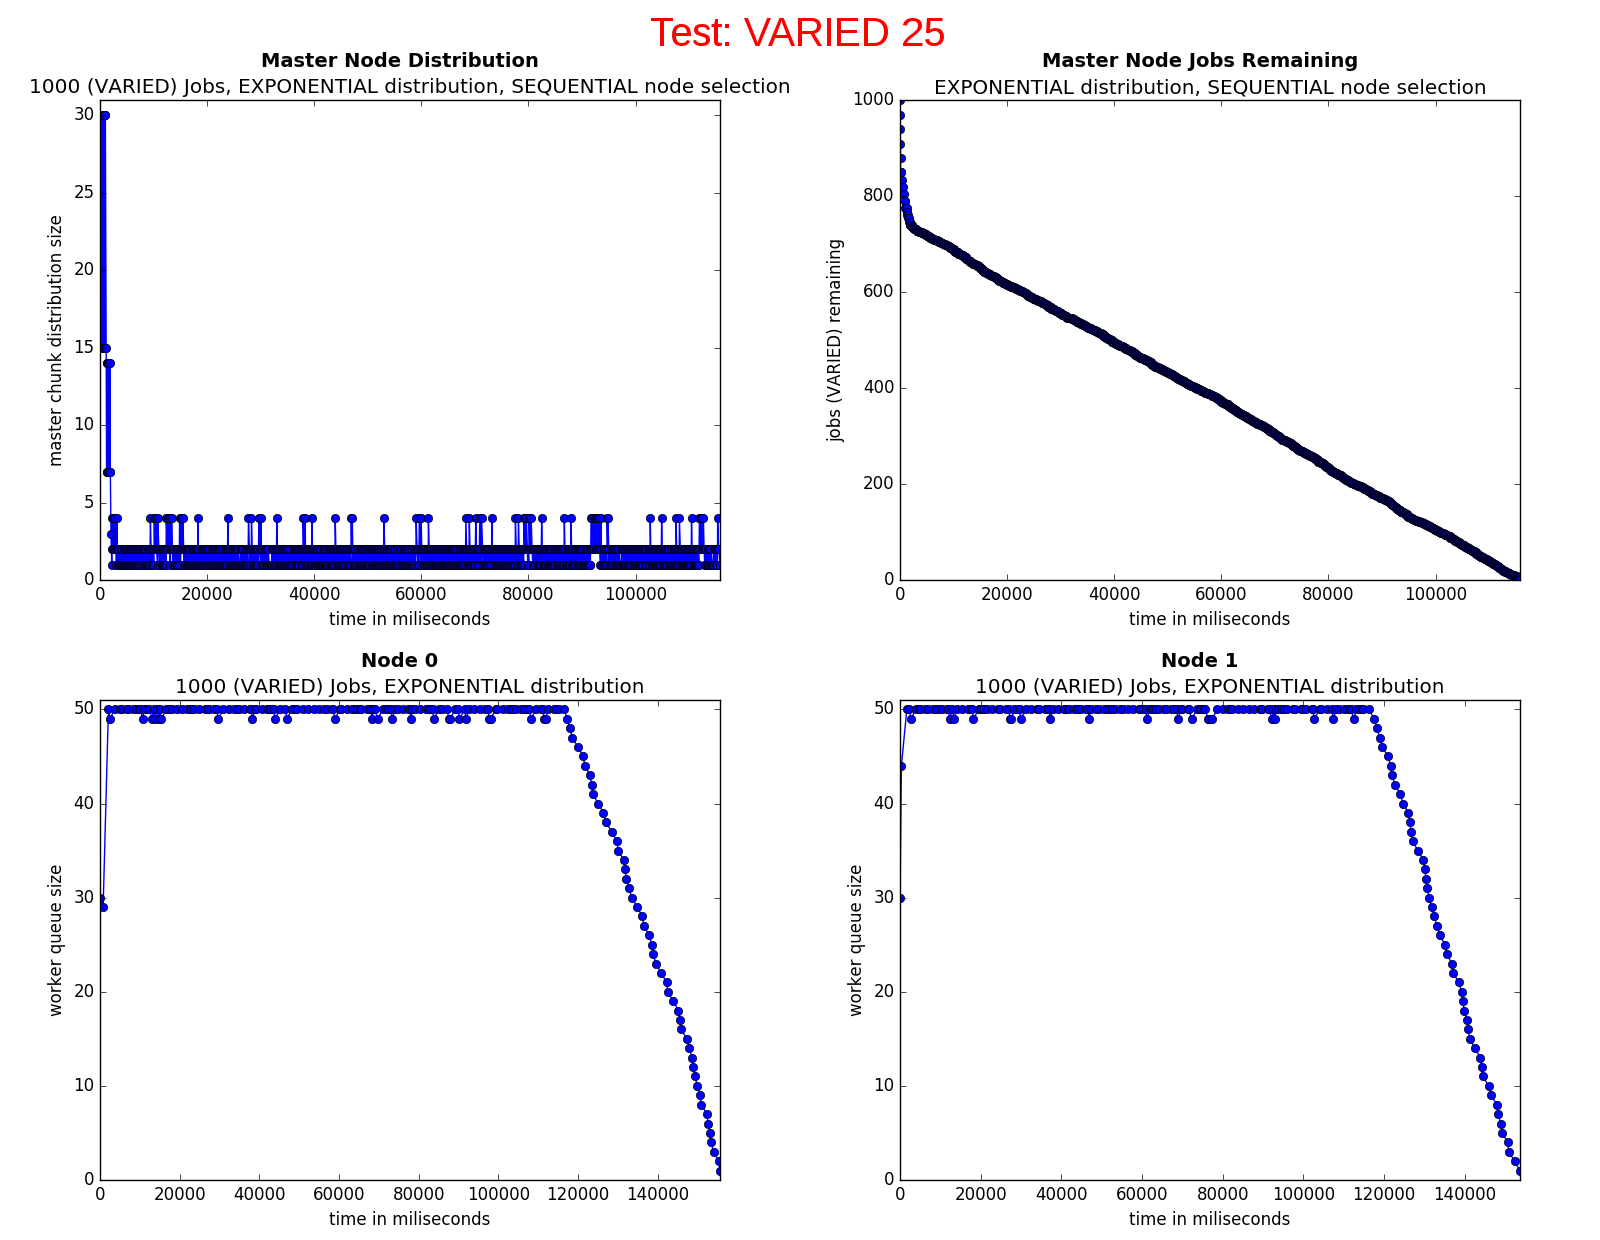
\includegraphics[width=1.2\linewidth]{combined_varied_overview/case_varied_25} }
    \caption{Sequential node selection, Exponential distribution} 
    \label{testVaried25} 
    \vspace{4ex}
  \end{subfigure}%% 
  \begin{subfigure}[b]{0.5\linewidth}
    \centering
    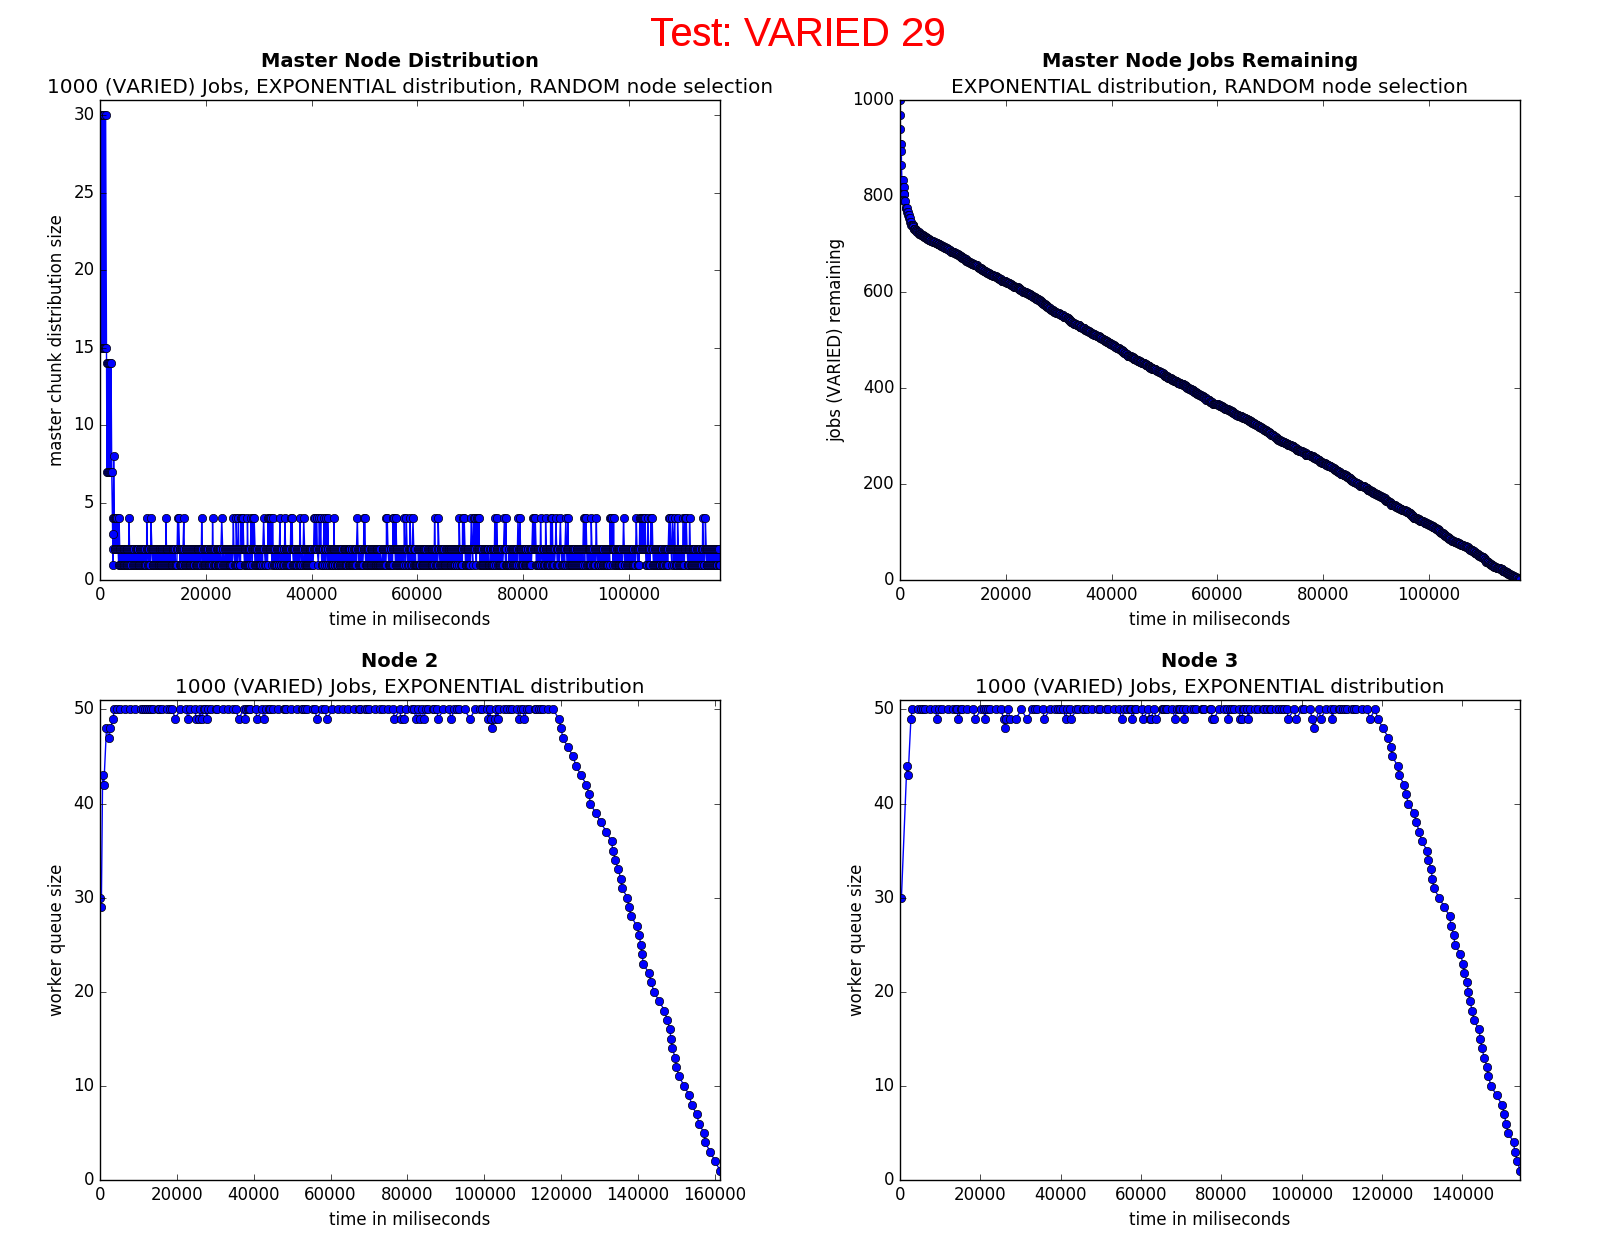
\includegraphics[width=1.2\linewidth]{combined_varied_overview/case_varied_29} 
    \caption{Random node selection, Exponential distribution} 
    \label{testVaried29} 
    \vspace{4ex}
  \end{subfigure} 
  
  
  \caption{Overview of simulation with 1000 varied jobs and 5 worker nodes part 2. These figures plot results for the varied test numbers 17, 21, 25, 29 as labeled at the top of each figure. The top left plot in each figure shows the master job distribution rate as time progresses. The top right plot in each figure shows the number of jobs remaining to distribute as time progresses. The bottom plots in each figure show queue sizes of two randomly selected workers.}
  \label{testsVaried17-29} 
  
\end{figure}

\begin{figure} 
\hspace*{9em}
\begin{subfigure}[b]{0.5\linewidth}
    \centering
    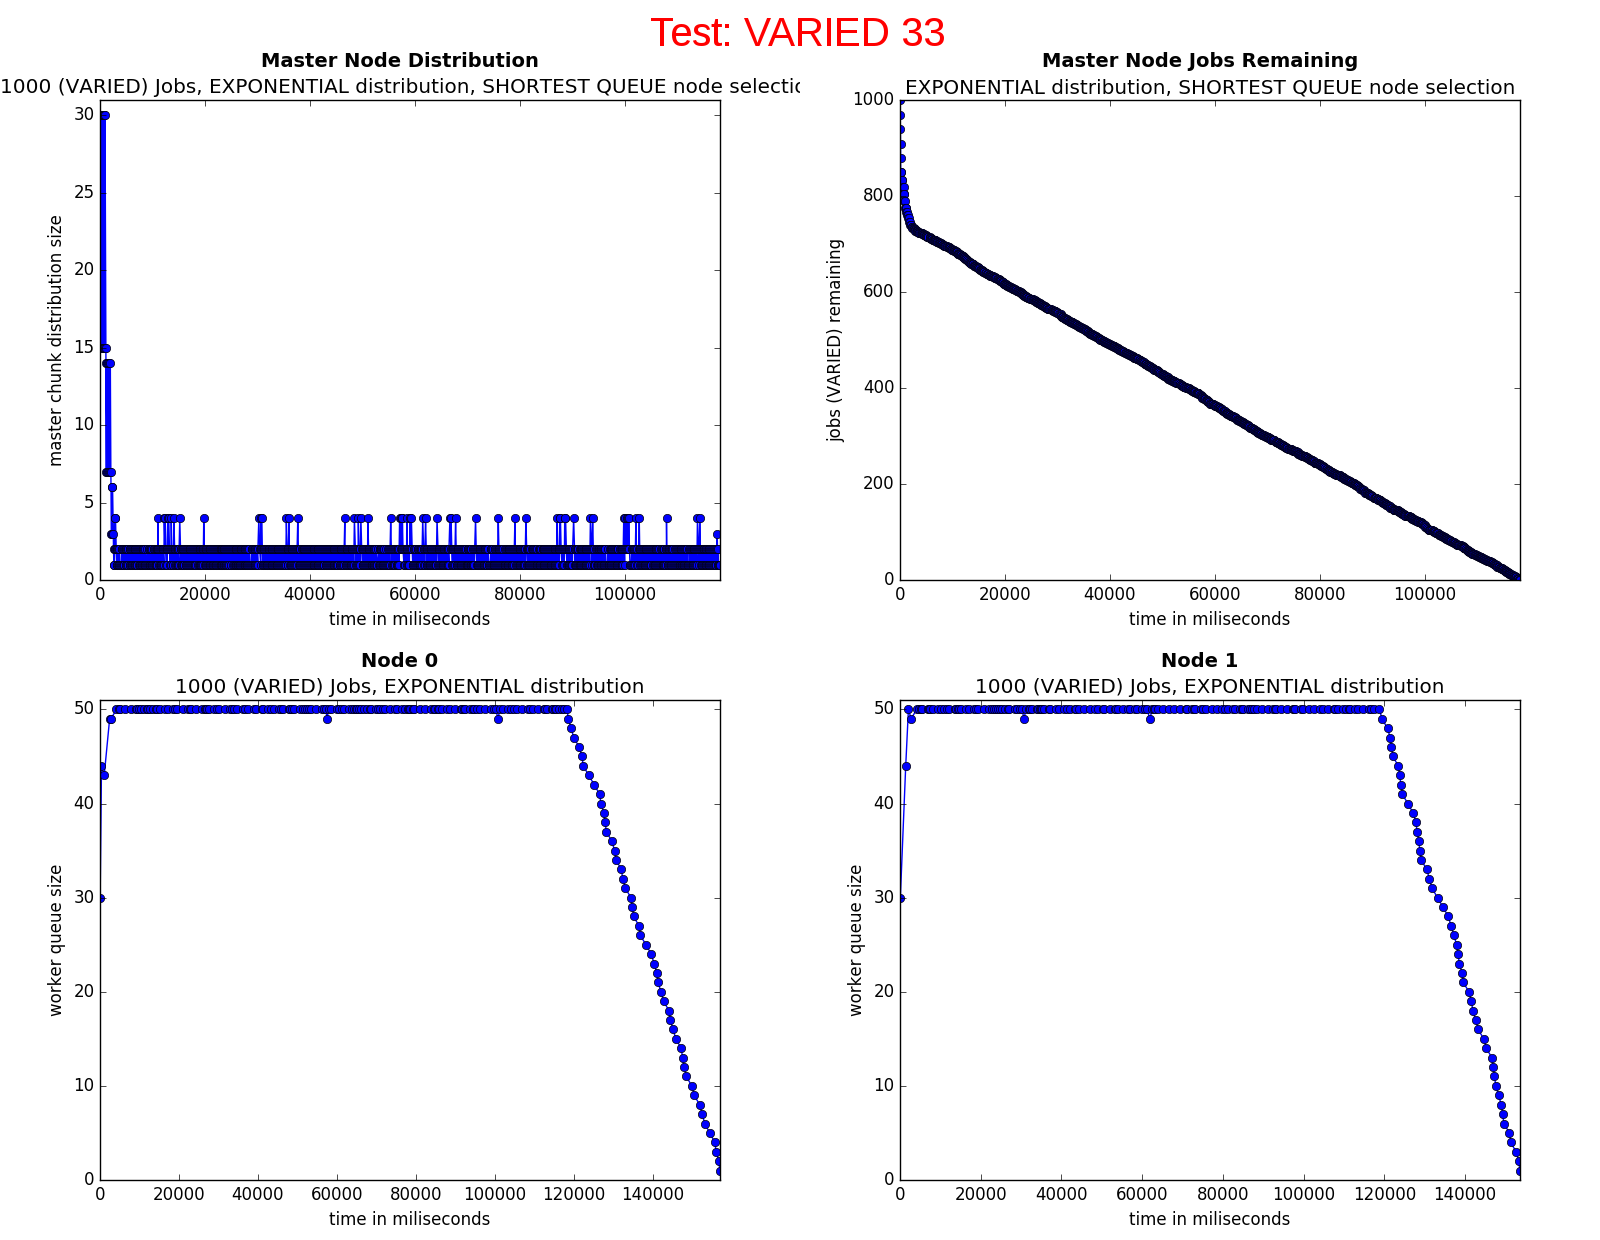
\includegraphics[scale=0.20]{combined_varied_overview/case_varied_33} 
    \caption{Shortest queue node selection, Exponential distribution} 
    \label{testVaried33} 
  \end{subfigure}

  \caption{Overview of simulation with 1000 varied jobs and 5 worker nodes part 3. This figure plot results for the varied test numbers 33 as labeled at the top of each figure. The top left plot in each figure shows the master job distribution rate as time progresses. The top right plot in each figure shows the number of jobs remaining to distribute as time progresses. The bottom plots in each figure show queue sizes of two randomly selected workers.}
  \label{testVaried33Figure} 
\end{figure}
%============================== END VARIED OverView FIGURES
%============================================================



%============================== START VARIED Linear FIGURES
%============================================================
\begin{figure}[p] 
  \begin{subfigure}[b]{0.5\linewidth}
    \centering
    \hbox{\hspace{-5.0em} \includegraphics[width=1.2\linewidth]{combined_varied_growing_workers_linear/case_varied_1} }
    \caption{5 workers}
    \label{testLinearVaried5} 
    \vspace{4ex}
  \end{subfigure}%% 
  \begin{subfigure}[b]{0.5\linewidth}
    \centering
    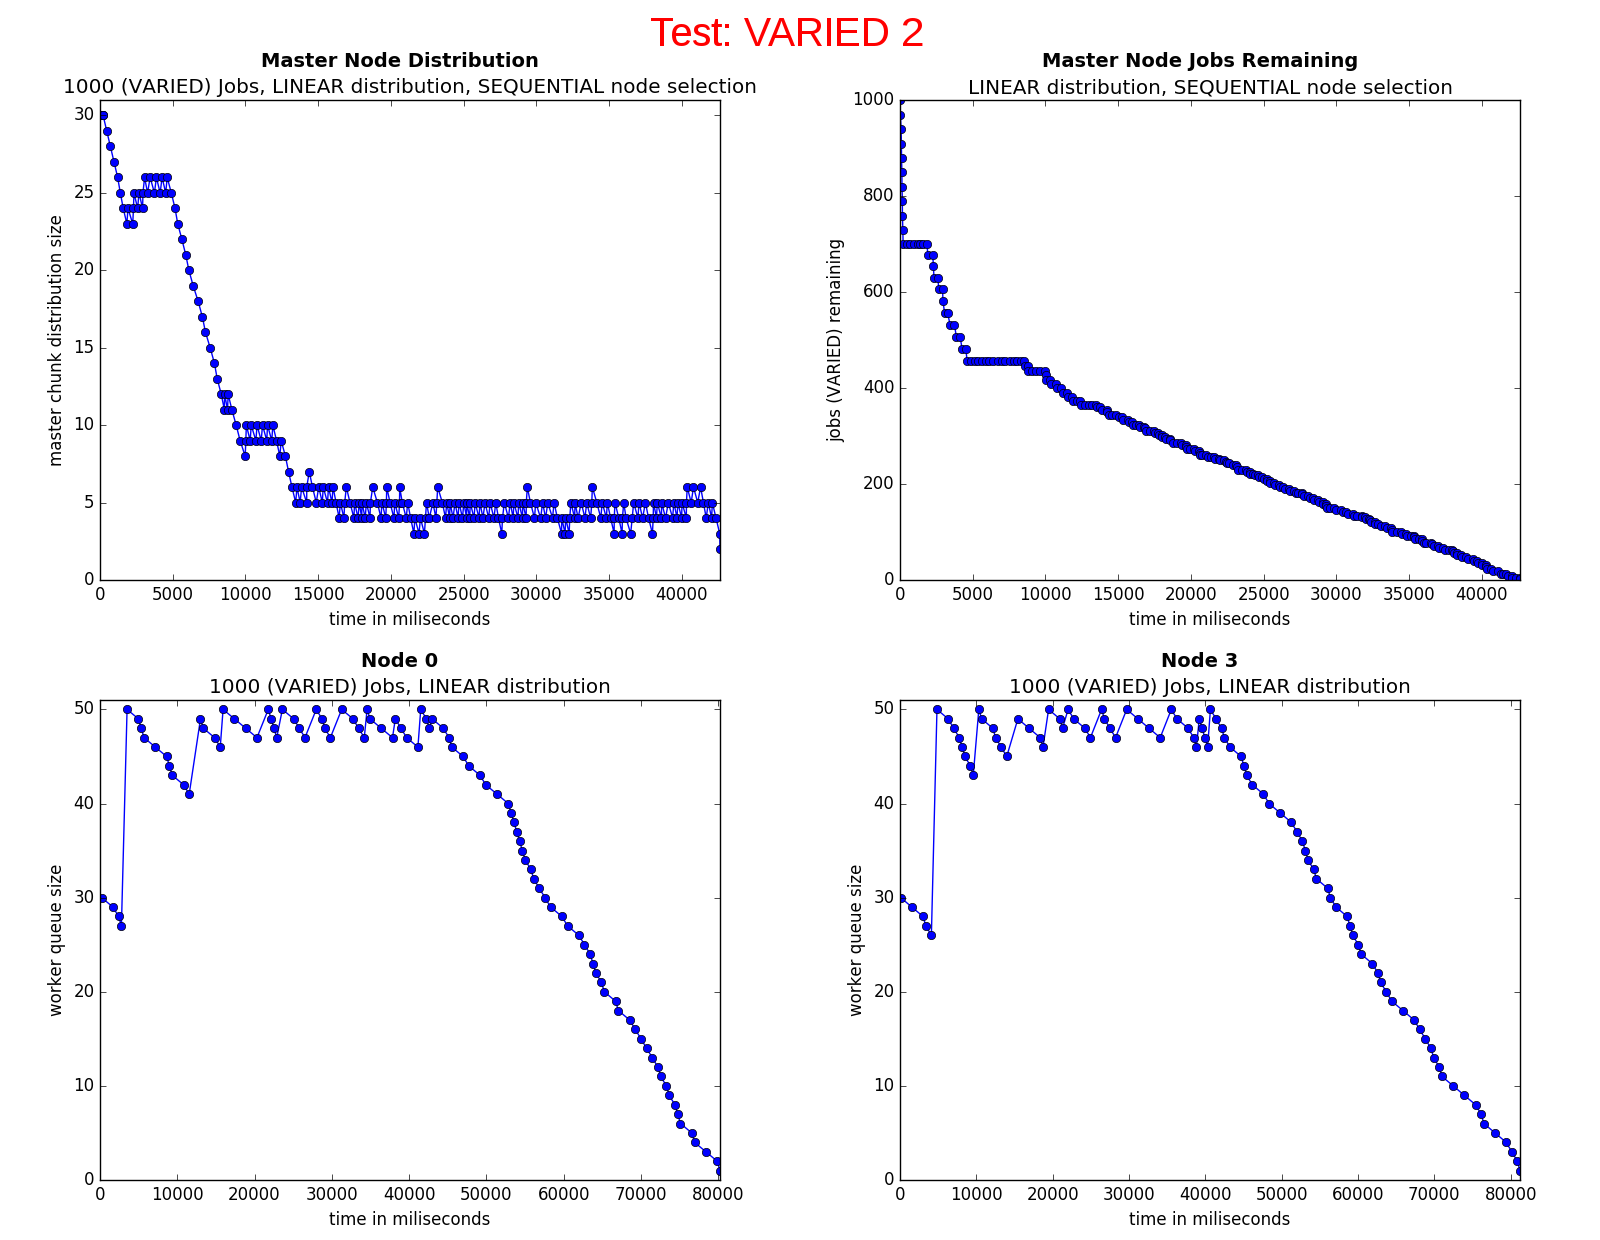
\includegraphics[width=1.2\linewidth]{combined_varied_growing_workers_linear/case_varied_2} 
    \caption{10 workers} 
    \label{testLinearVaried10} 
    \vspace{4ex}
  \end{subfigure} 
  
  
  \begin{subfigure}[b]{0.5\linewidth}
    \centering
    \hbox{\hspace{-5.0em} 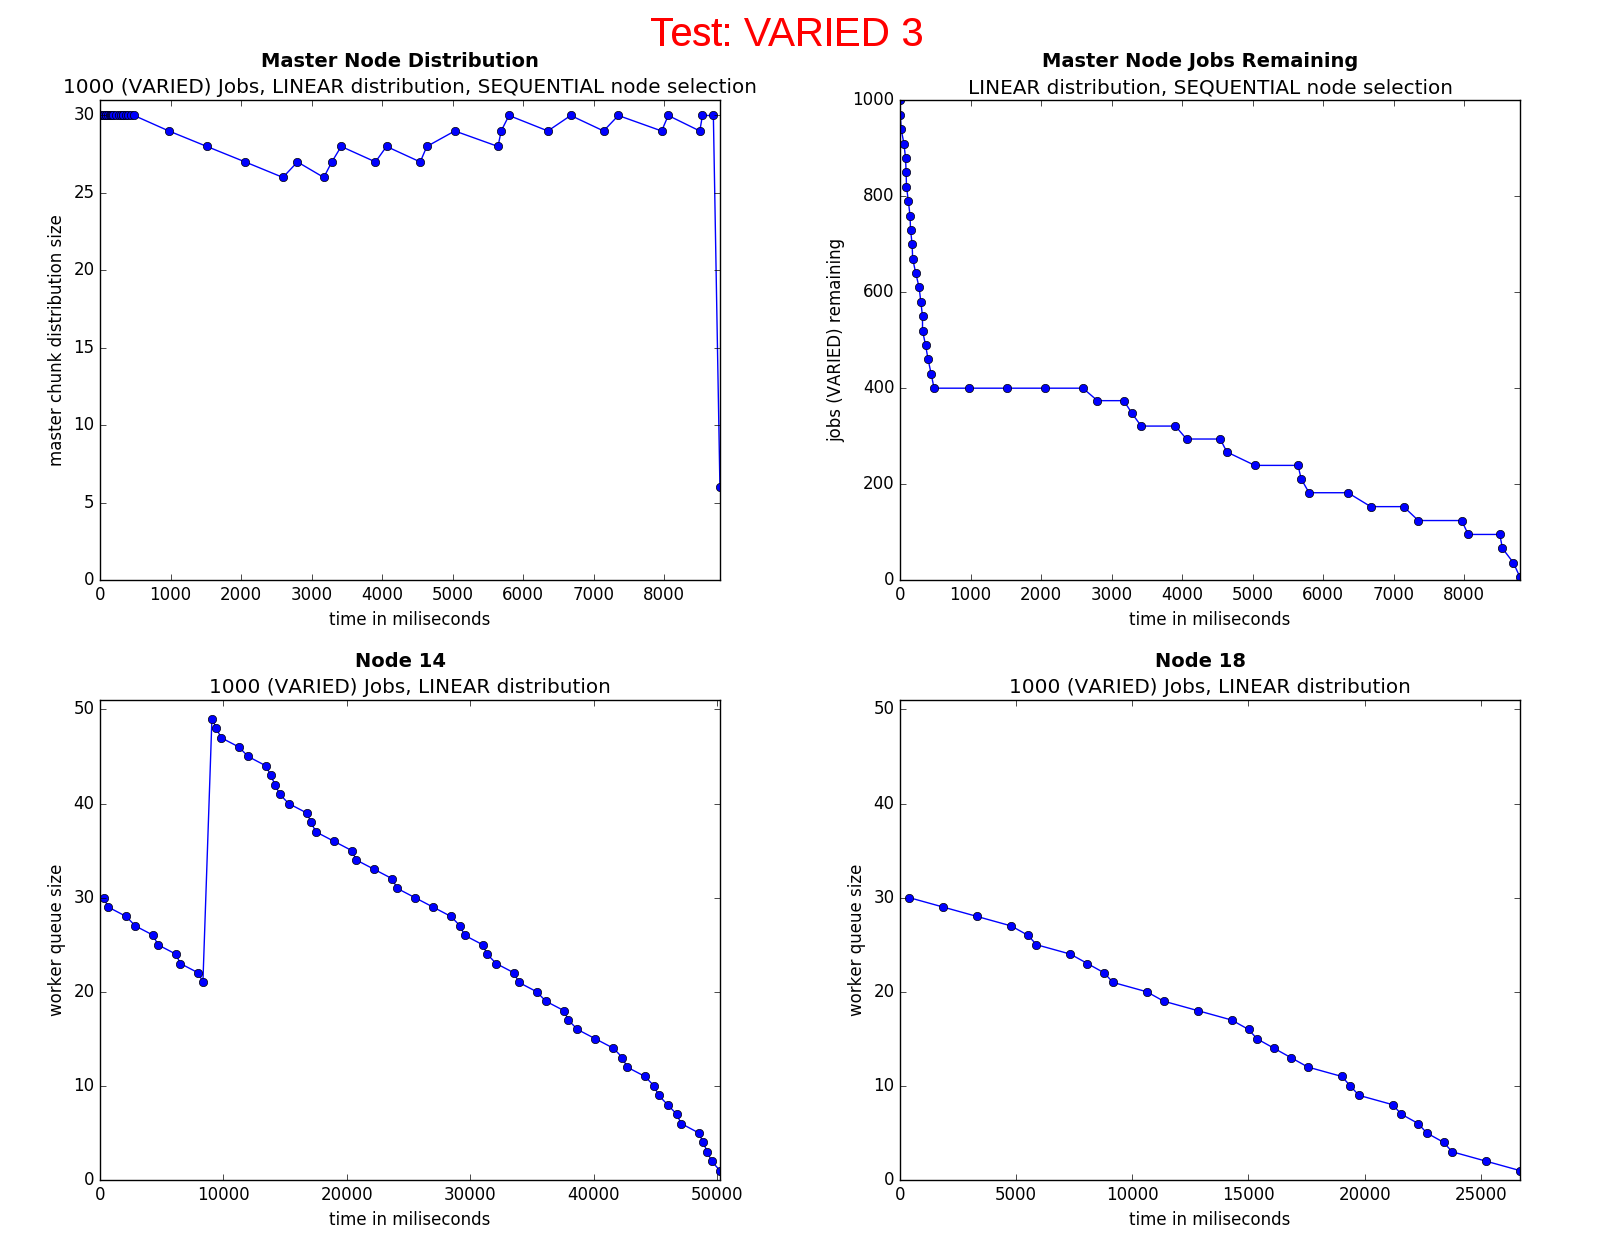
\includegraphics[width=1.2\linewidth]{combined_varied_growing_workers_linear/case_varied_3} }
    \caption{20 workers} 
    \label{testLinearVaried20} 
    \vspace{4ex}
  \end{subfigure}%% 
  \begin{subfigure}[b]{0.5\linewidth}
    \centering
    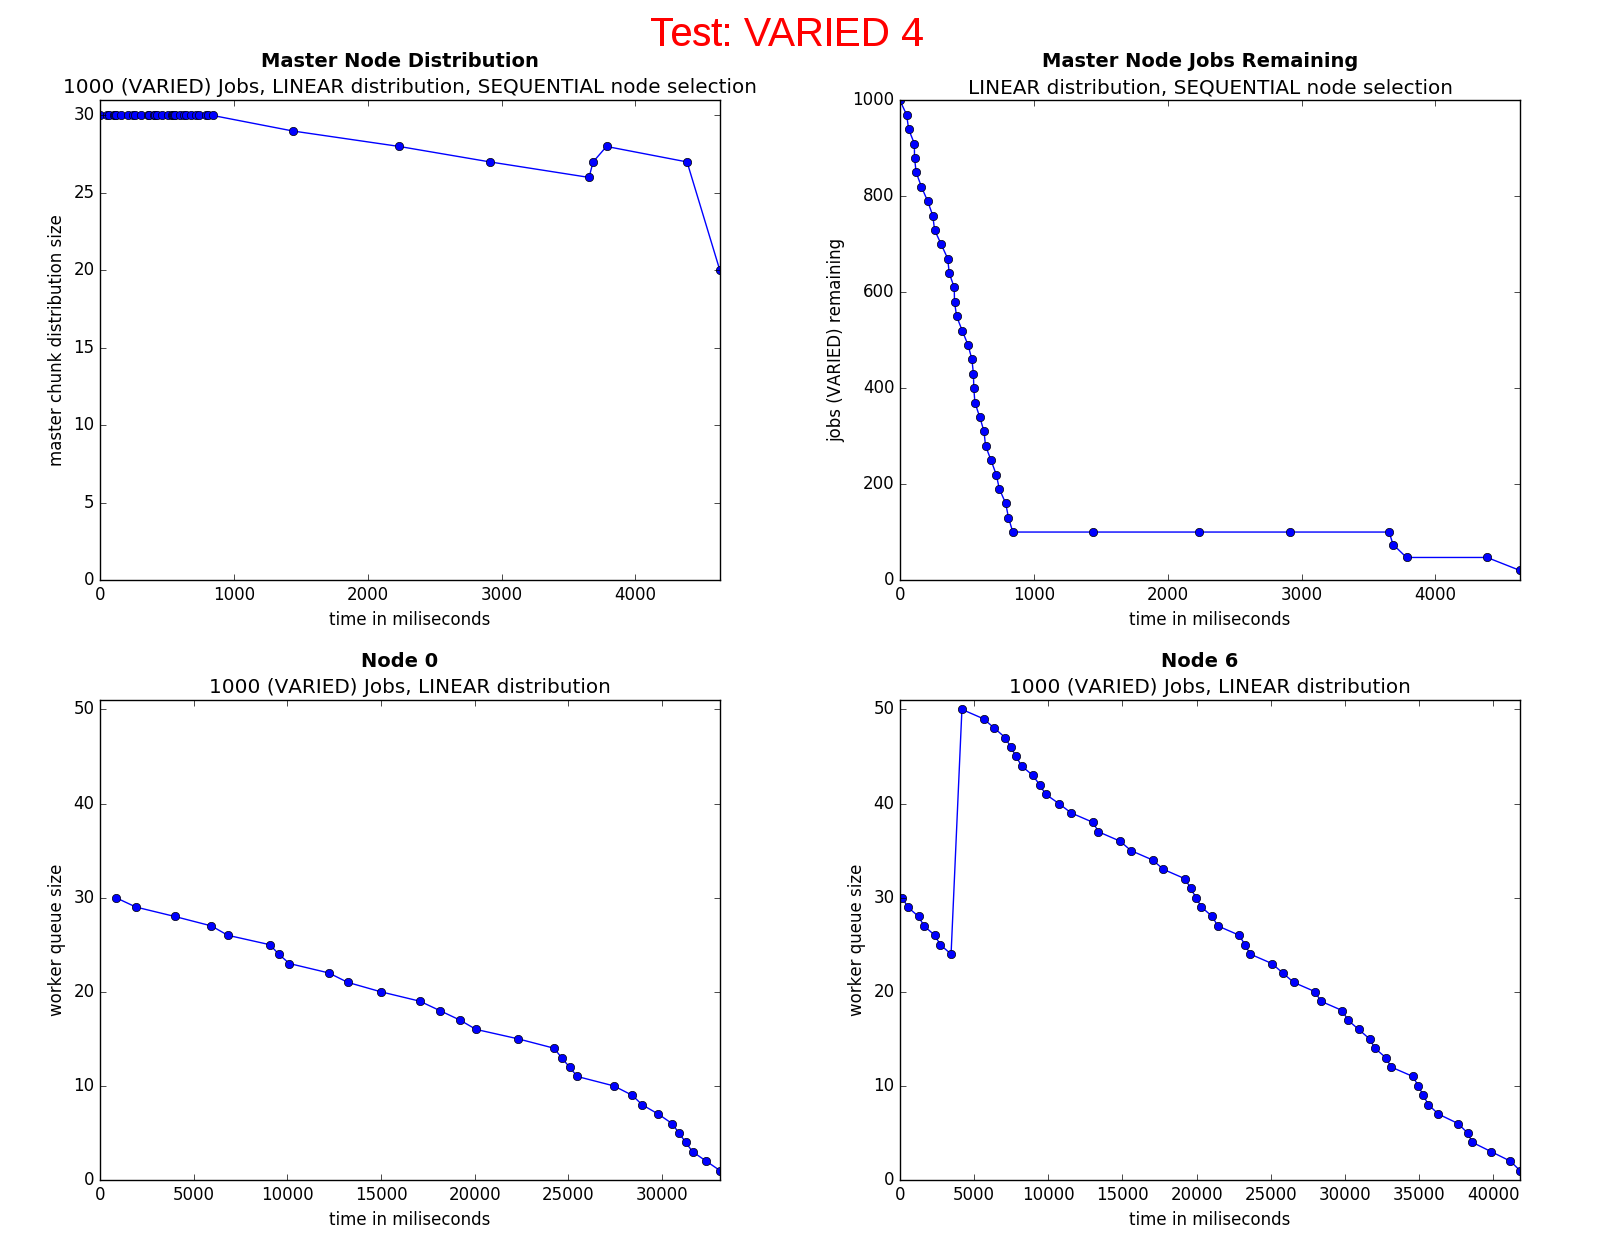
\includegraphics[width=1.2\linewidth]{combined_varied_growing_workers_linear/case_varied_4} 
    \caption{30 workers} 
    \label{testLinearVaried30} 
    \vspace{4ex}
  \end{subfigure} 
  
  
  \caption{These tests focus on linear job chunk distribution with 1000 varied jobs to process and varying worker size. These figures plot results for the varied test numbers 1, 2, 3, 4 as labeled at the top of each figure. The top left plot in each figure shows the master job distribution rate as time progresses. The top right plot in each figure shows the number of jobs remaining to distribute as time progresses. The bottom plots in each figure show queue sizes of two randomly selected workers.}
  \label{testsVariedLinear} 
  
\end{figure}
%============================== END VARIED Linear FIGURES
%================================================================





%============================== START VARIED Exponential FIGURES
%=================================================================
\begin{figure}
  \begin{subfigure}[b]{0.5\linewidth}
    \centering
    \hbox{\hspace{-5.0em} 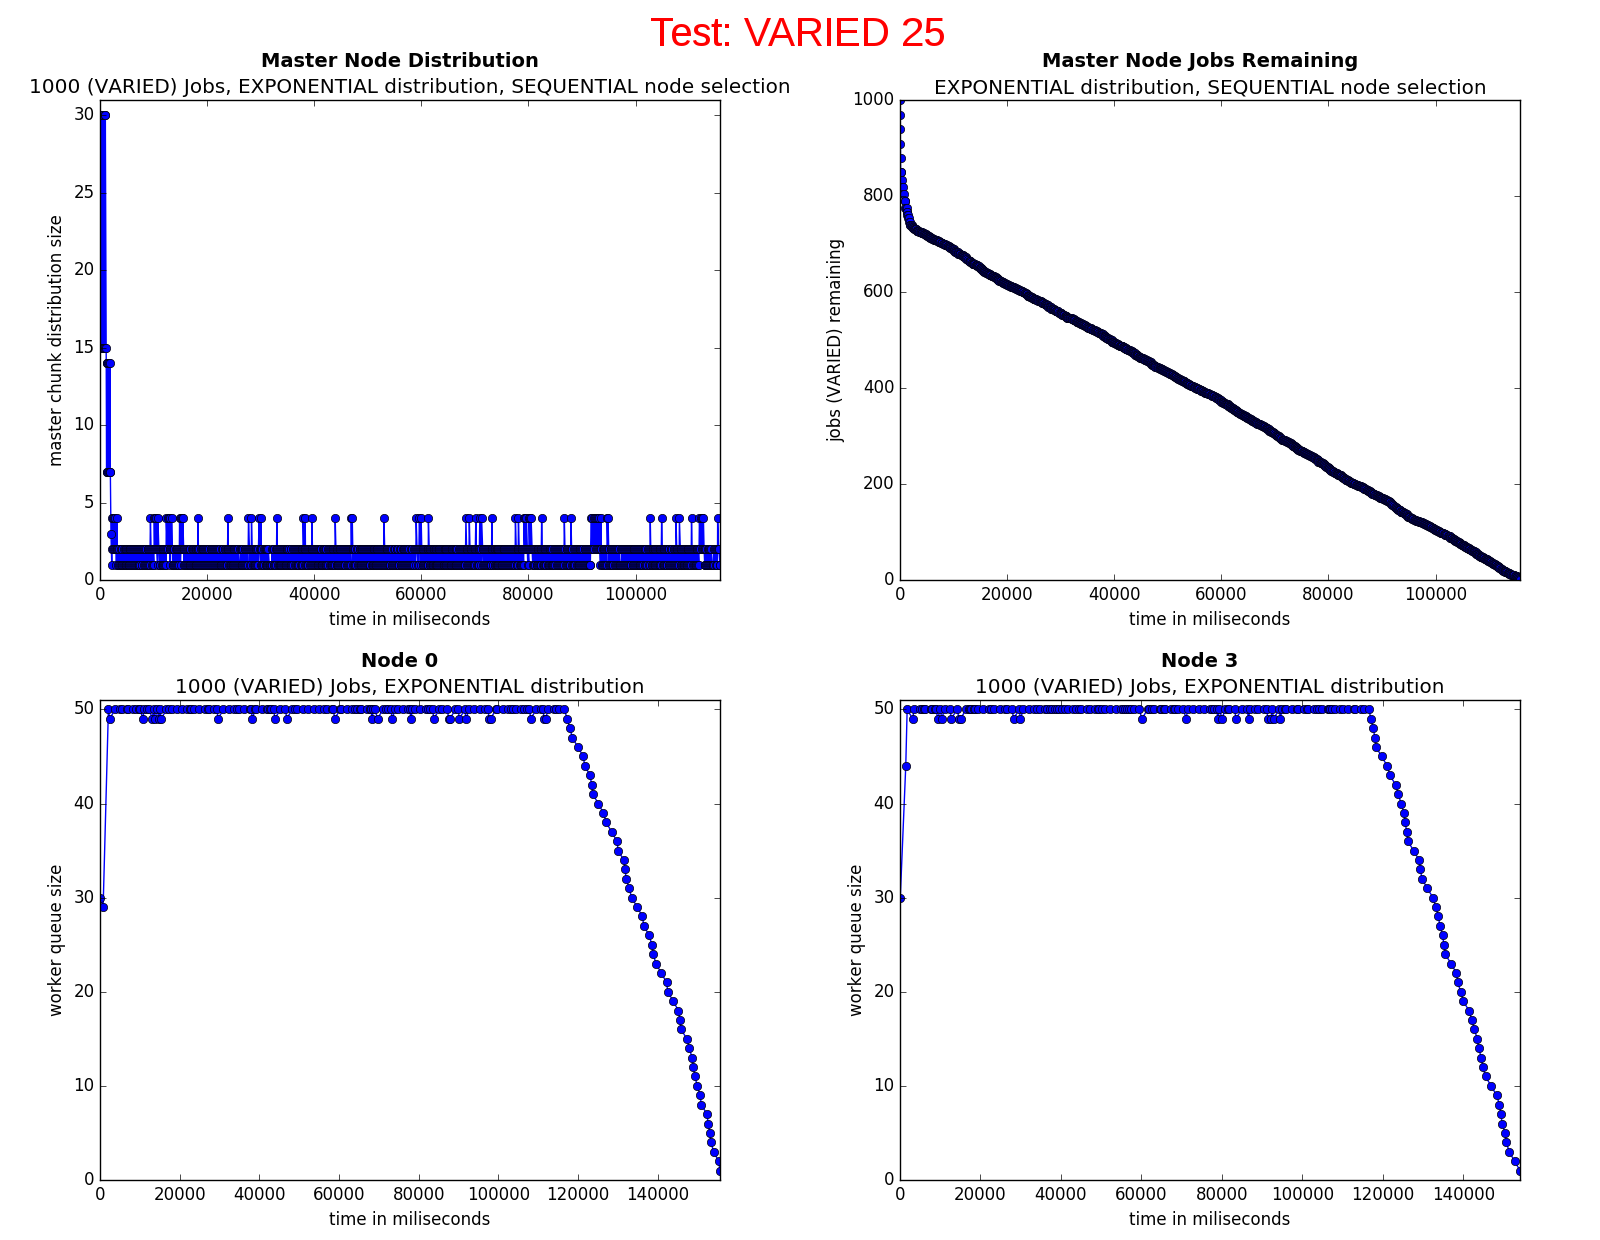
\includegraphics[width=1.2\linewidth]{combined_varied_growing_workers_exp/case_varied_25} }
    \caption{5 workers}
    \label{testExpVaried5} 
    \vspace{4ex}
  \end{subfigure}%% 
  \begin{subfigure}[b]{0.5\linewidth}
    \centering
    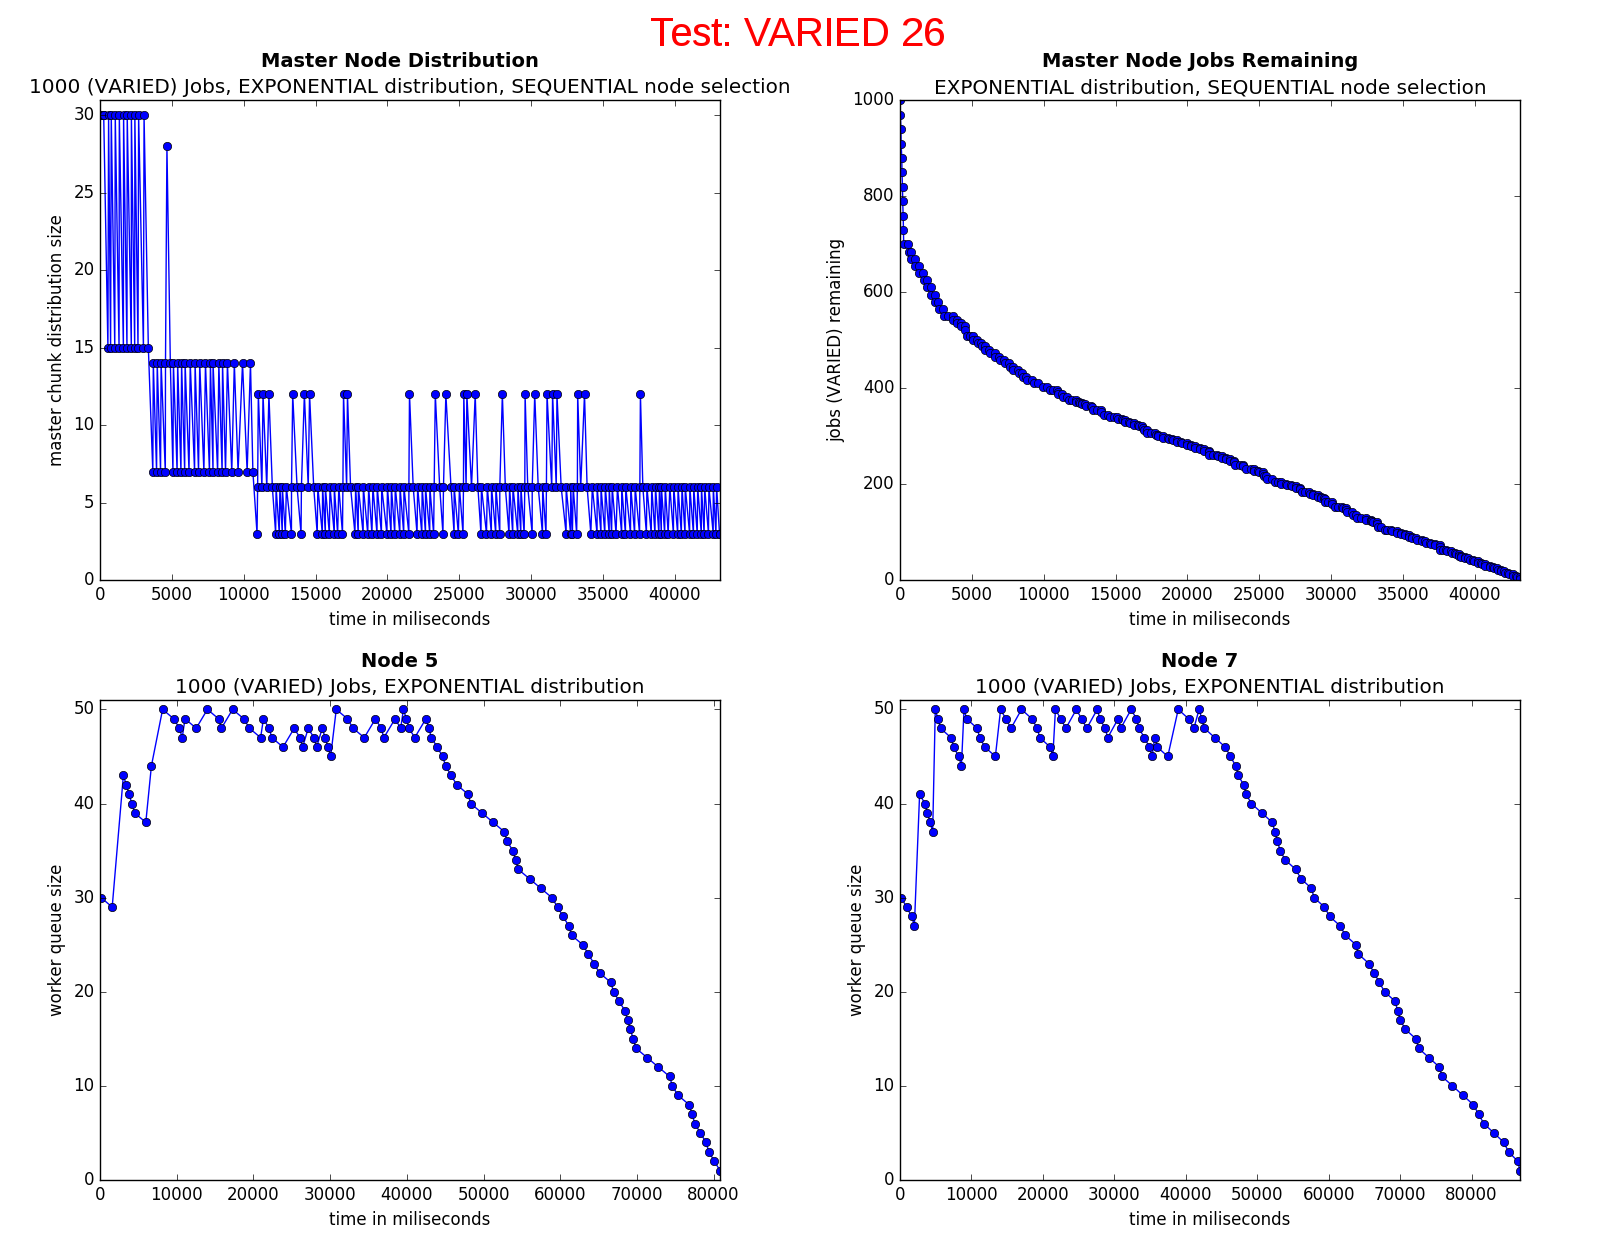
\includegraphics[width=1.2\linewidth]{combined_varied_growing_workers_exp/case_varied_26} 
    \caption{10 workers} 
    \label{testExpVaried10} 
    \vspace{4ex}
  \end{subfigure} 
  
  
  \begin{subfigure}[b]{0.5\linewidth}
    \centering
    \hbox{\hspace{-5.0em} 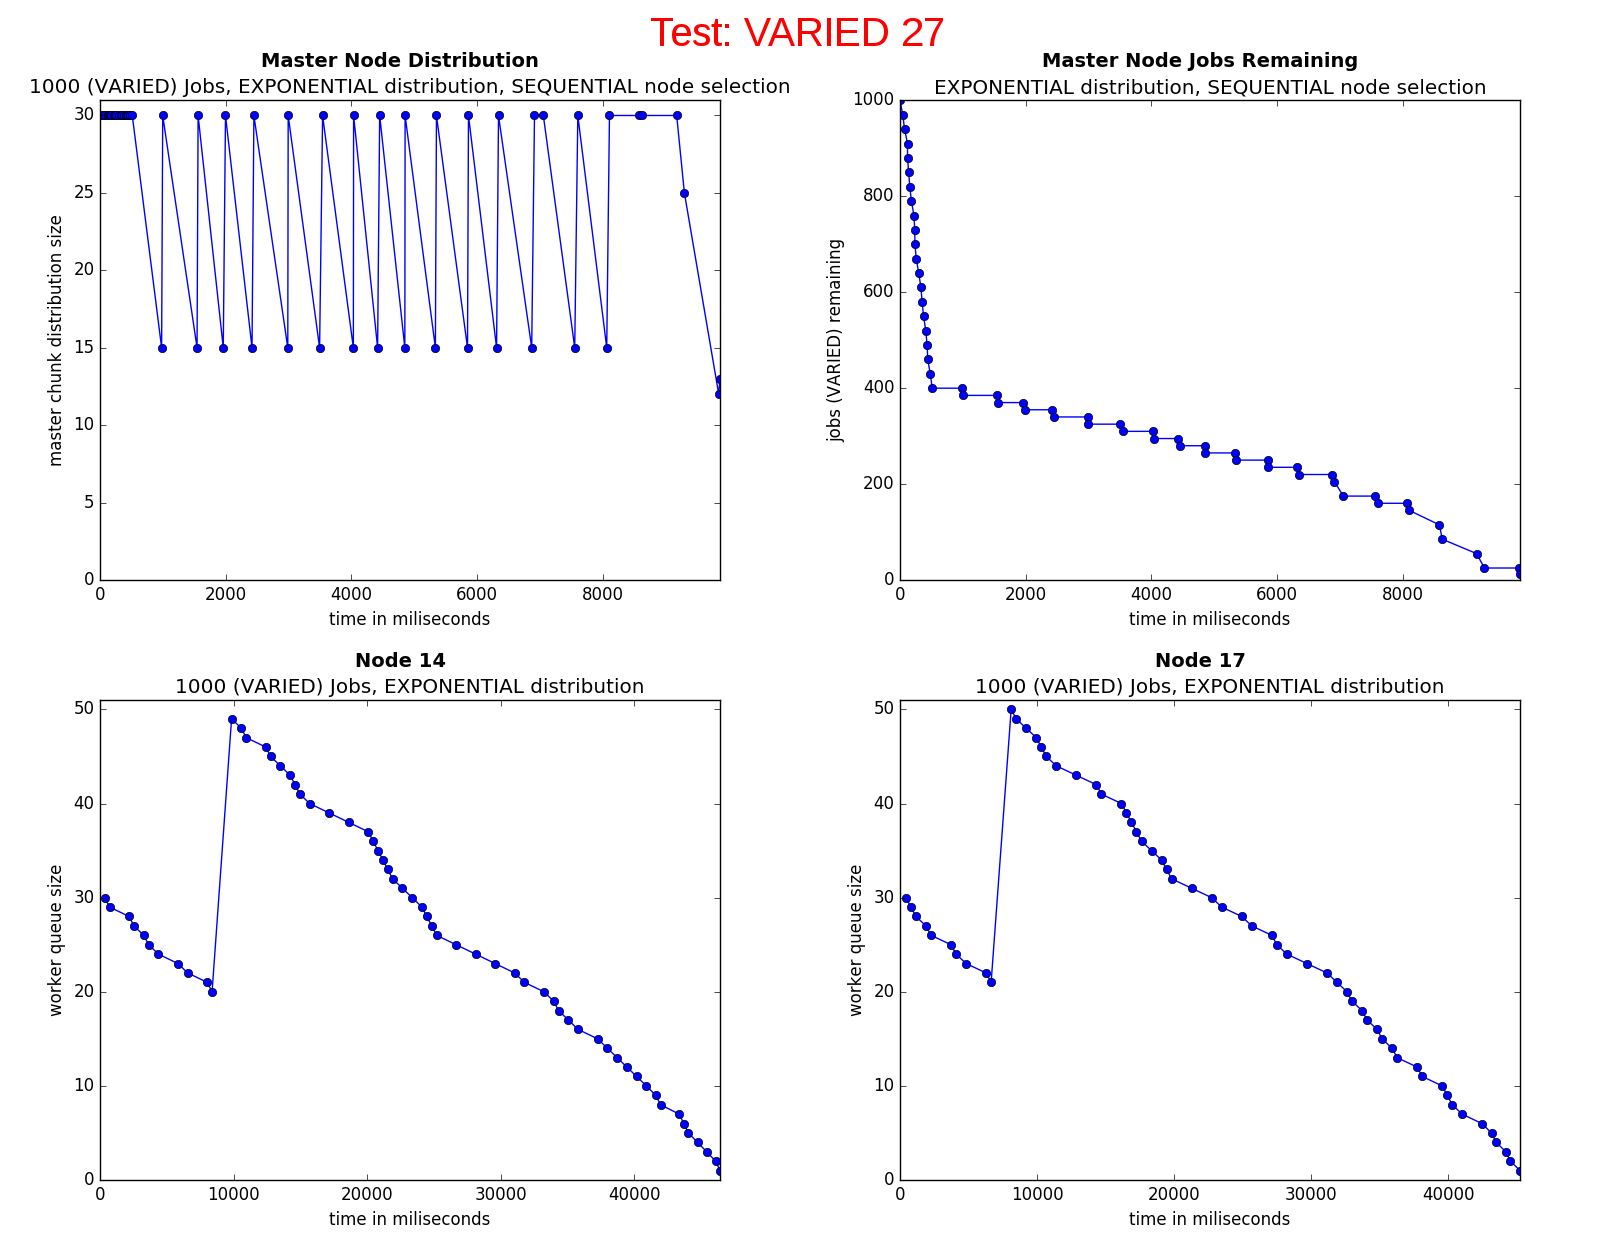
\includegraphics[width=1.2\linewidth]{combined_varied_growing_workers_exp/case_varied_27} }
    \caption{20 workers} 
    \label{testExpVaried20} 
    \vspace{4ex}
  \end{subfigure}%% 
  \begin{subfigure}[b]{0.5\linewidth}
    \centering
    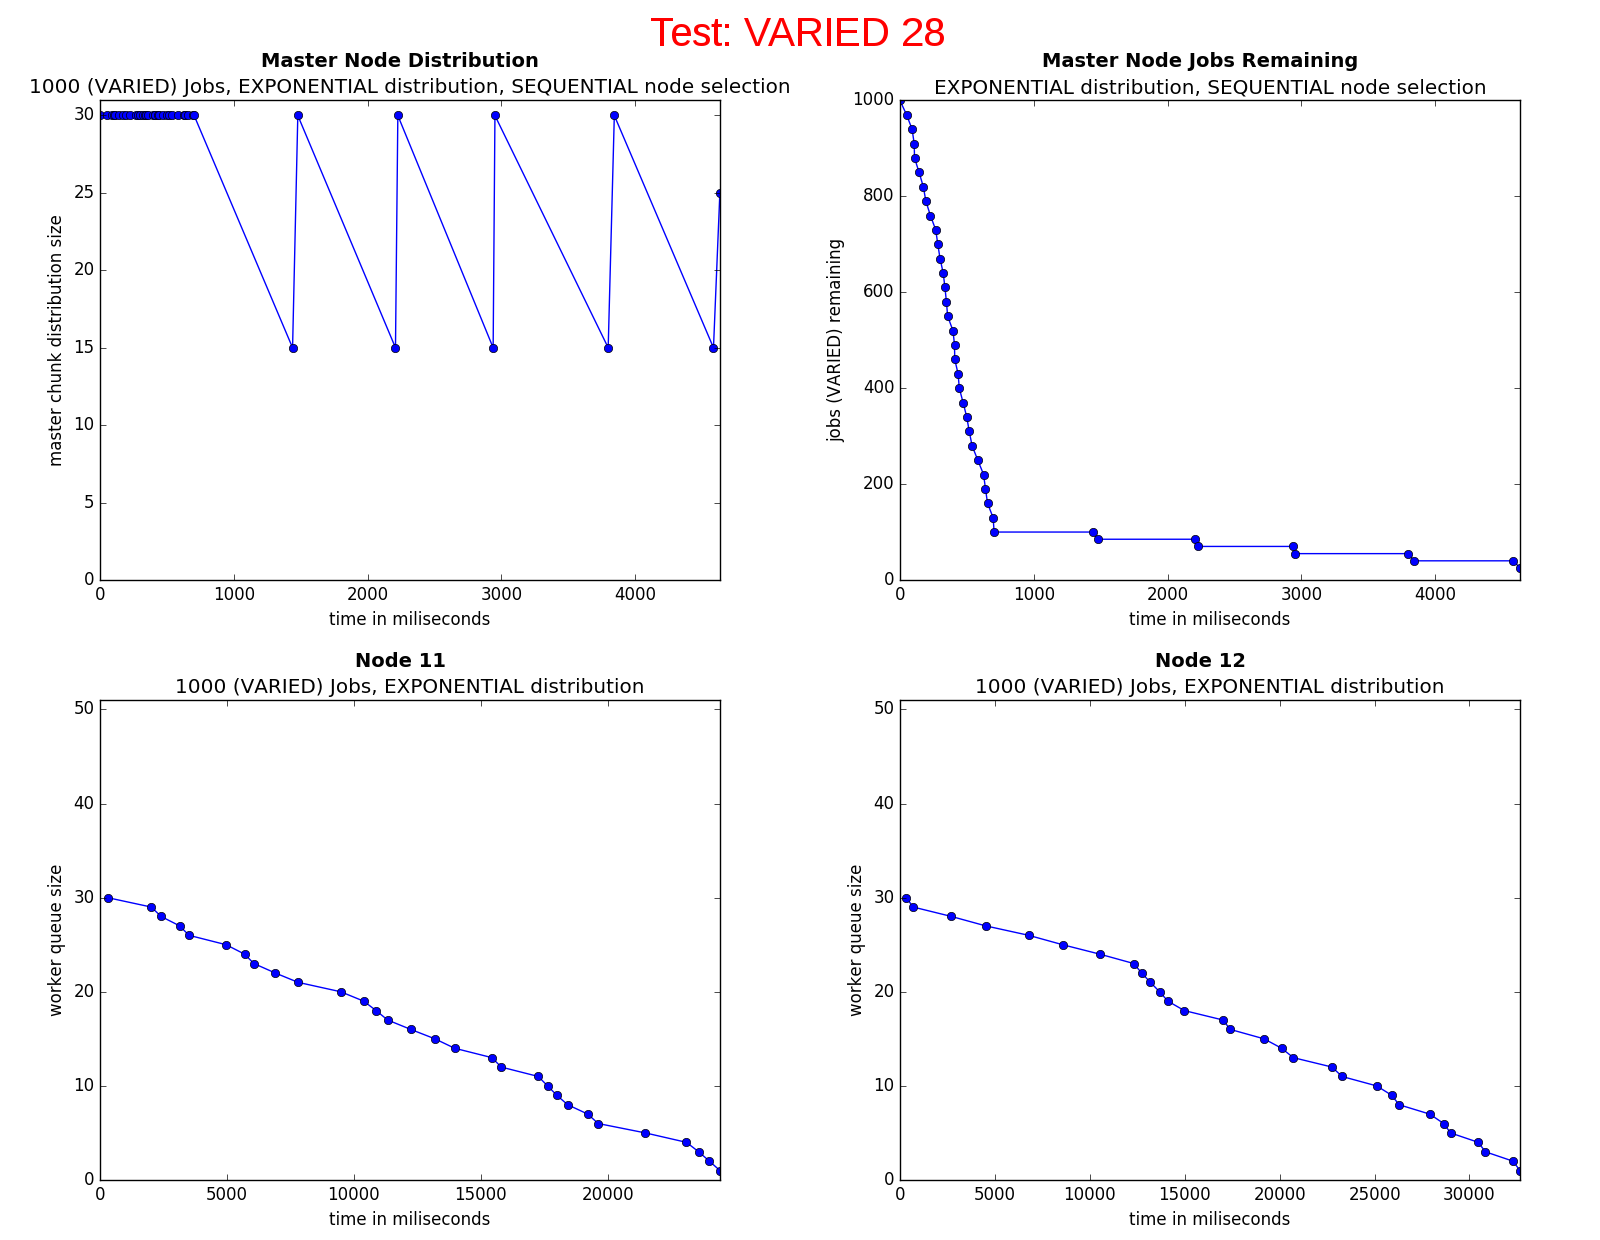
\includegraphics[width=1.2\linewidth]{combined_varied_growing_workers_exp/case_varied_28} 
    \caption{30 workers} 
    \label{testExpVaried30} 
    \vspace{4ex}
  \end{subfigure} 
  
  
  \caption{These tests focus on exponential job chunk distribution with 1000 varied jobs to process and varying worker size. These figures plot results for the varied test numbers 25, 26, 27, 28 as labeled at the top of each figure. The top left plot in each figure shows the master job distribution rate as time progresses. The top right plot in each figure shows the number of jobs remaining to distribute as time progresses. The bottom plots in each figure show queue sizes of two randomly selected workers.}
  \label{testsVariedExp} 
  
\end{figure}
%============================== END VARIED Exponential FIGURES
%================================================================



%============================== START VARIED Constant FIGURES
%=================================================================
\begin{figure}[p] 
  \begin{subfigure}[b]{0.5\linewidth}
    \centering
    \hbox{\hspace{-5.0em} 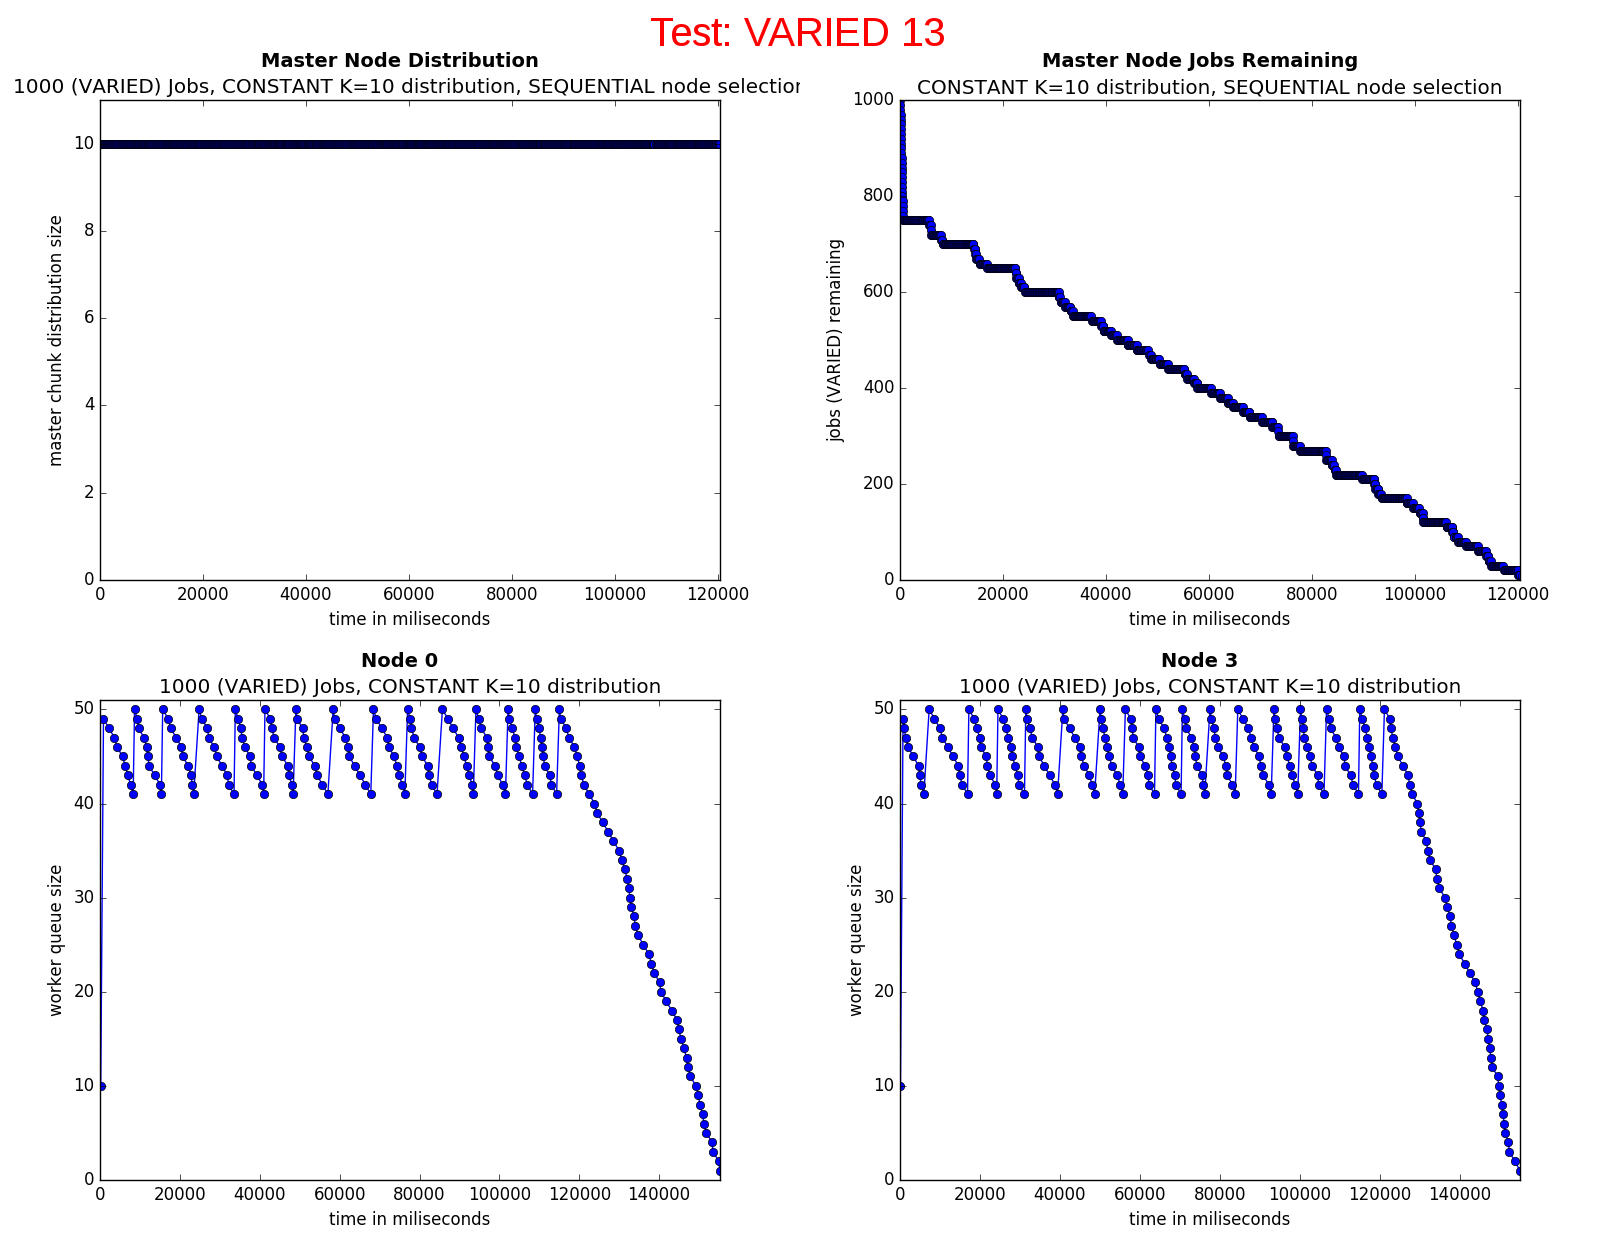
\includegraphics[width=1.2\linewidth]{combined_varied_growing_workers_constant/case_varied_13} }
    \caption{5 workers}
    \label{testConstantVaried5} 
    \vspace{4ex}
  \end{subfigure}%% 
  \begin{subfigure}[b]{0.5\linewidth}
    \centering
    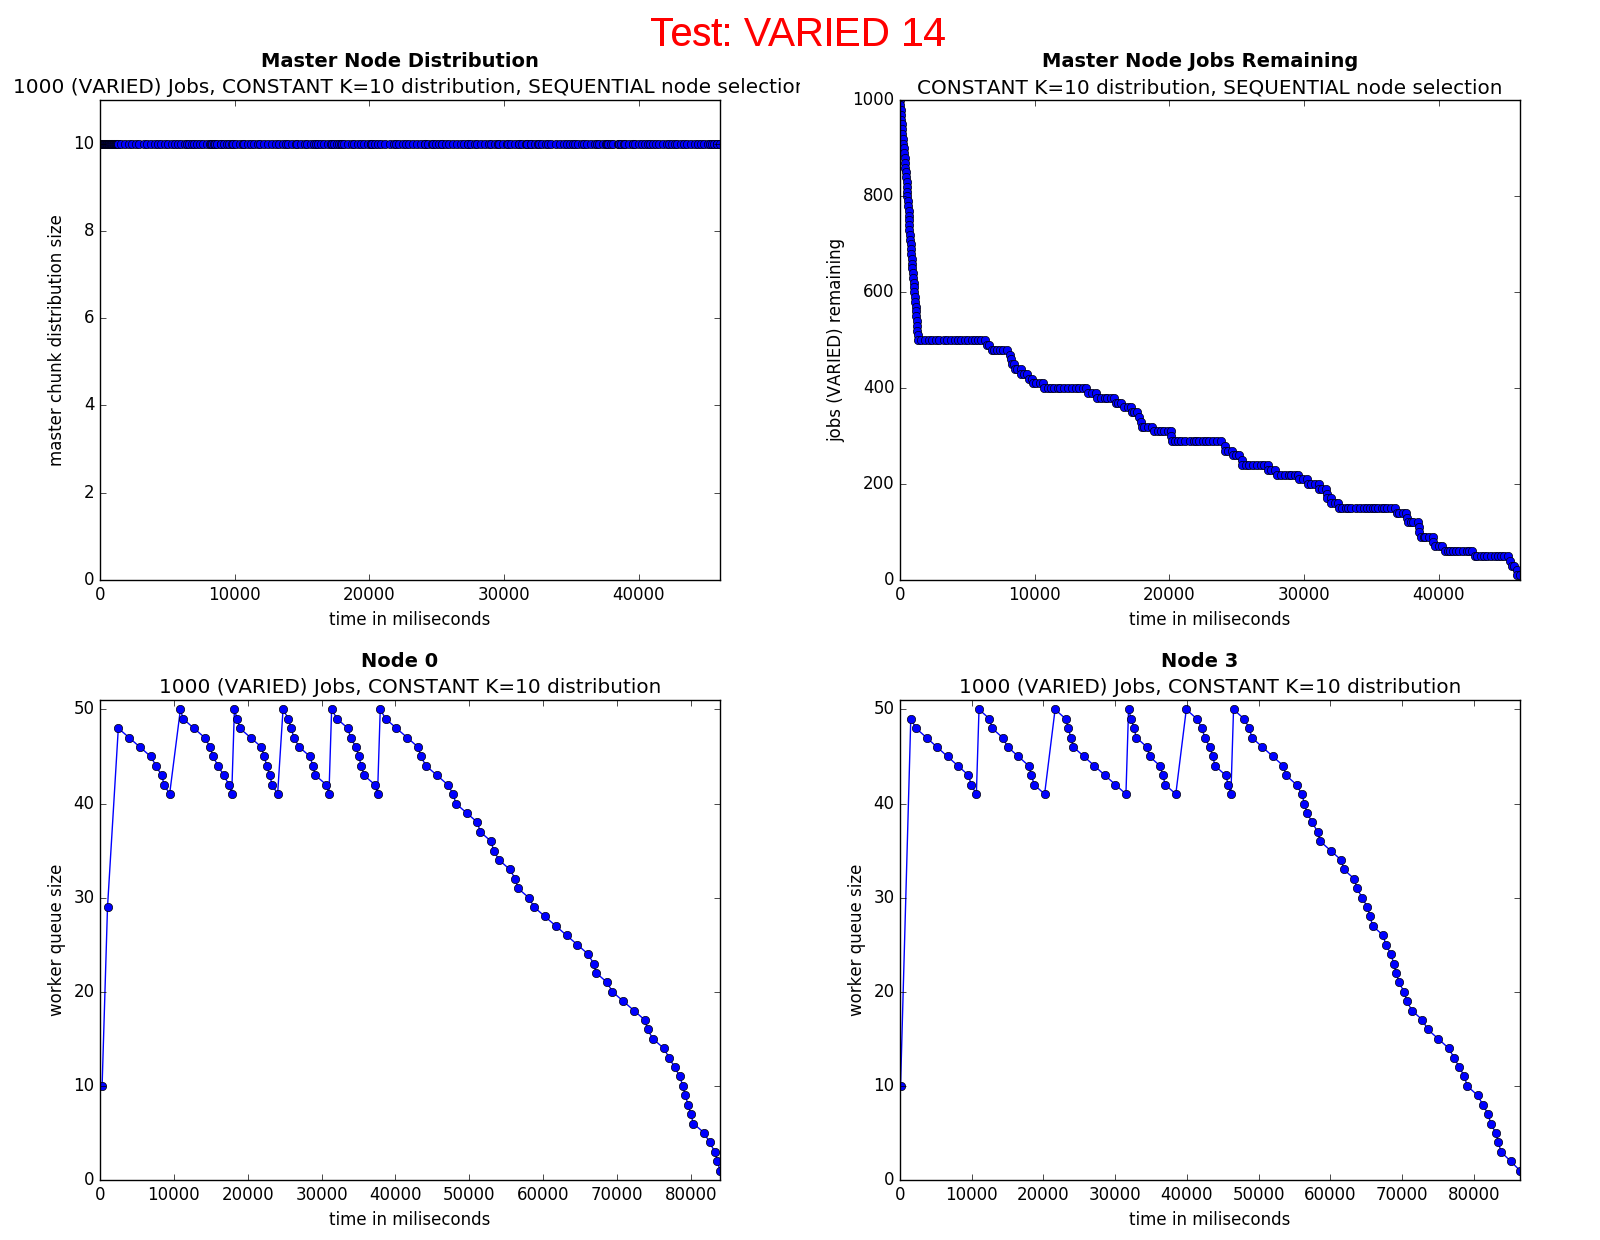
\includegraphics[width=1.2\linewidth]{combined_varied_growing_workers_constant/case_varied_14} 
    \caption{10 workers} 
    \label{testConstantVaried10} 
    \vspace{4ex}
  \end{subfigure} 
  
  
  \begin{subfigure}[b]{0.5\linewidth}
    \centering
    \hbox{\hspace{-5.0em} 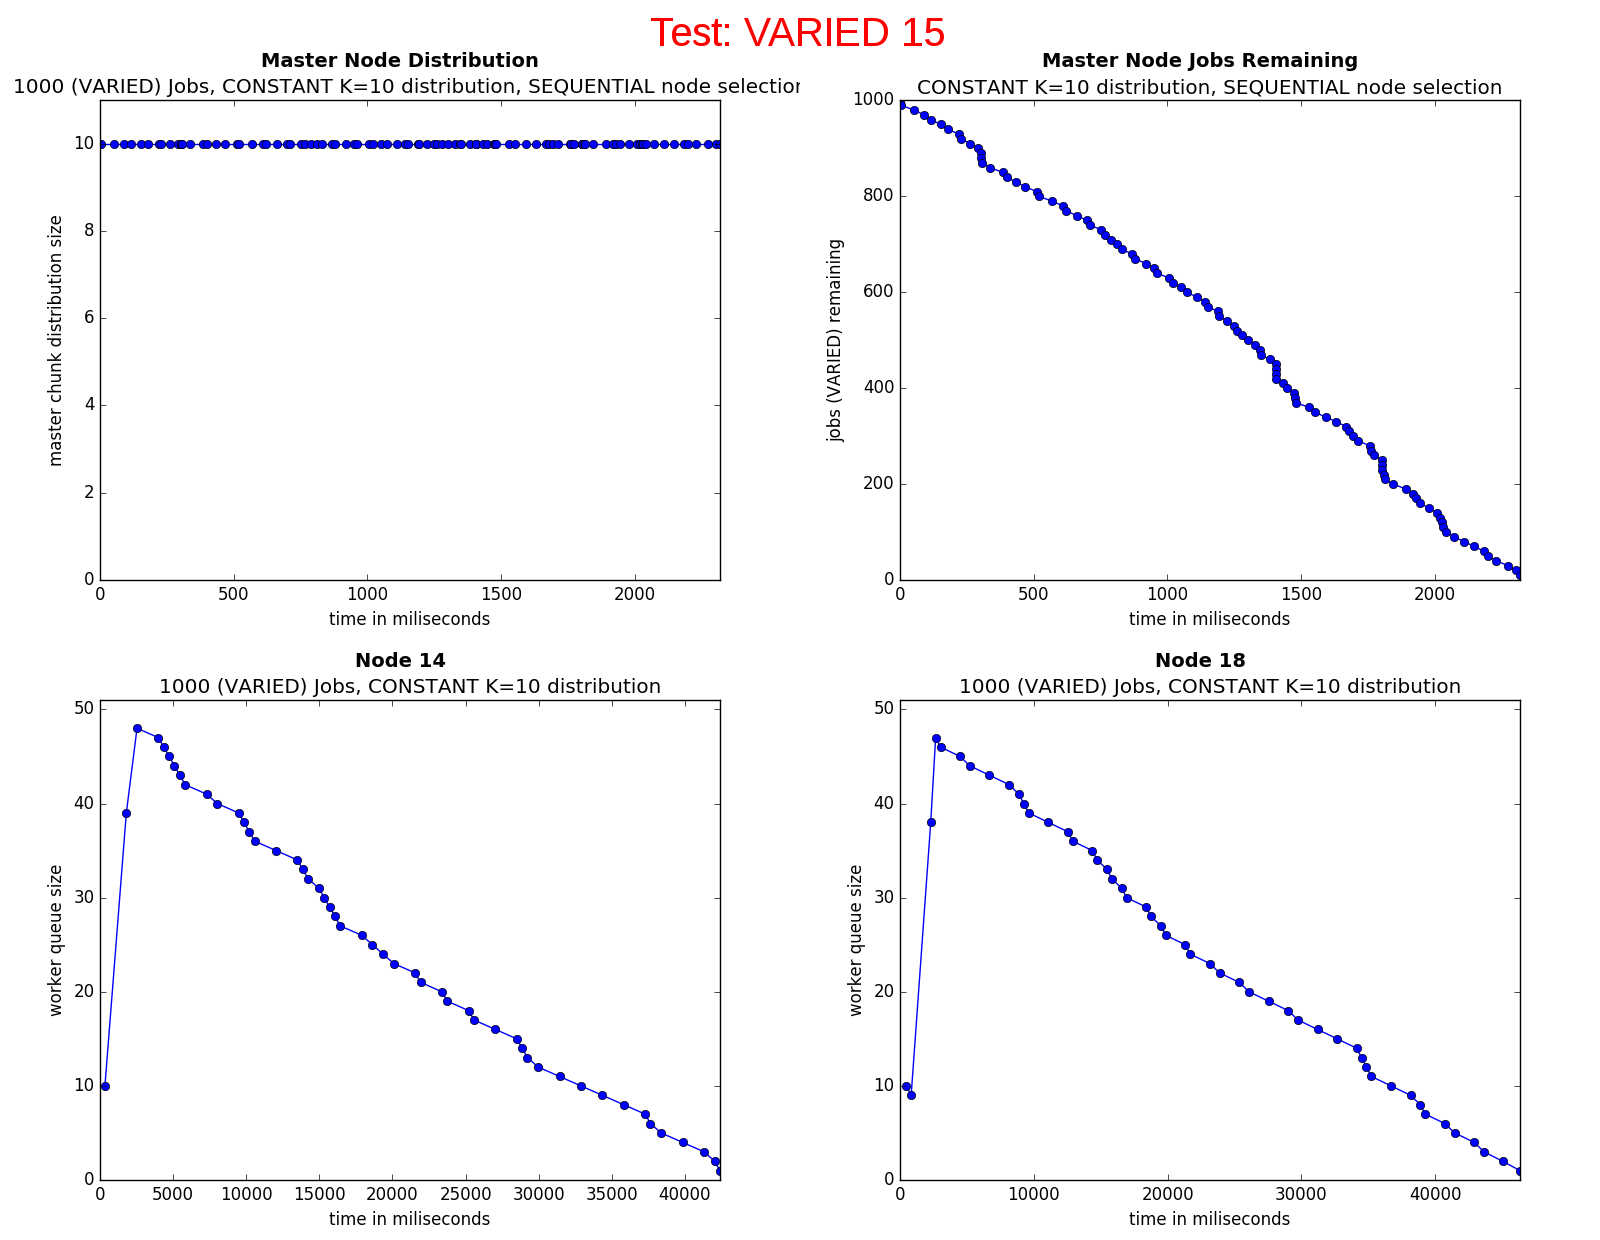
\includegraphics[width=1.2\linewidth]{combined_varied_growing_workers_constant/case_varied_15} }
    \caption{20 workers} 
    \label{testConstantVaried20} 
    \vspace{4ex}
  \end{subfigure}%% 
  \begin{subfigure}[b]{0.5\linewidth}
    \centering
    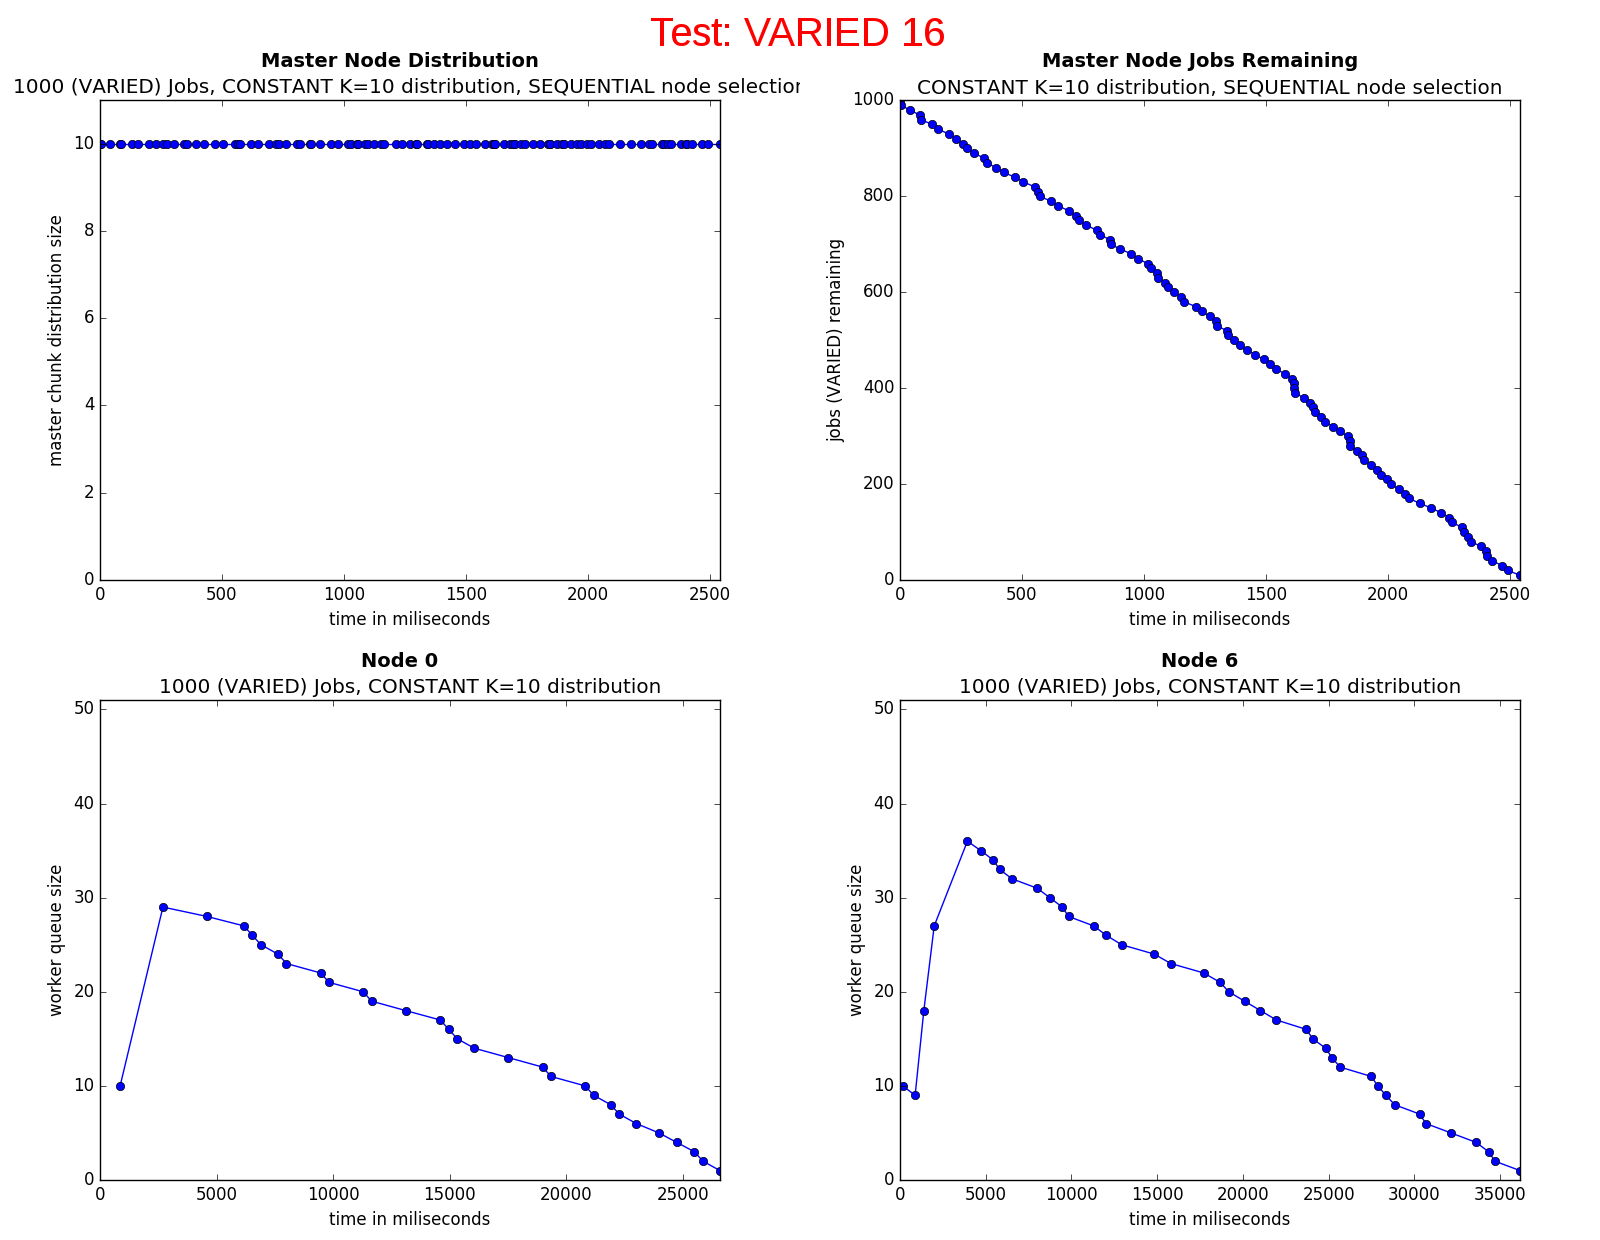
\includegraphics[width=1.2\linewidth]{combined_varied_growing_workers_constant/case_varied_16} 
    \caption{30 workers} 
    \label{testConstantVaried30} 
    \vspace{4ex}
  \end{subfigure} 
  
  
  \caption{These tests focus on constant job chunk distribution with 1000 varied jobs to process and varying worker size. These figures plot results for the varied test numbers 13, 14, 15, 16 as labeled at the top of each figure. The top left plot in each figure shows the master job distribution rate as time progresses. The top right plot in each figure shows the number of jobs remaining to distribute as time progresses. The bottom plots in each figure show queue sizes of two randomly selected workers.}
  \label{testsVariedConstant} 
  
\end{figure}
%============================== END VARIED Constant FIGURES
%=============================================================

\clearpage
\section{Future Work} \label{futureWork}
This simulation focused on varying two configurations while keeping others constant. As the next steps, it would be beneficial to vary some of the configurations that were kept constant as shown in Table \ref{constantConfs}. Aside from varying configurations it would definitely be beneficial to setup a simulation in an actual distributed cluster, which should be somewhat trivial to setup through Amazon AWS. 

Additionally, this simulation studied the push method where the master continuously attempted to distribute, or push out, resources to the workers. It would be interesting to study the pull method where workers come to the master to receive more jobs. In this setup the configurations would clearly be different, but this scheduling strategy may prove to be beneficial in certain scenarios.

\section{Conclusion} \label{conclusion}
The results show that in workloads with very similar job execution times and workloads with varying job execution times, randomly selecting a worker node will have a detrimental effect. Additionally, it also seemed to be the case that constant job distribution yielded the fastest completion time in both workloads. Exponential and linear job distribution strategies ended up being more favorable for spreading job load evenly across workers when there is a relatively small number of workers available. When there is an abundant number of workers, constant job distribution strategy tended to spread the job load evenly as it is less likely to make worker queues suddenly jump to higher sizes. Thus overall, when faced with distributing jobs in a cluster of uniform nodes, the following generalizations could be made based on the presented results:
\begin{itemize}
  \item Random worker node selection tends to have a detrimental effect.
  \item If strictly looking for best performance, distribute a constant number of jobs at all times.
  \item If looking for ideal workload spread, distribute a constant number of jobs when there is an abundant number of workers, and vary the distribution in a linear or exponential rate when there are a few workers available.

\end{itemize}


%%%%%%%%%%%
% References
%%%%%%%%%%%
\bibliographystyle{plain}
\bibliography{PEECbib}

\end{document}
